\begin{enumerate}
\item {\bf \underline{Writing something every day.}}
\item describe the fast 3D -> 2D projection algorithm.
\item add follow-me result in.
\item describe multiple-pass of ABPA. This is useful for complicated structures, nested, blocked, etc.
\item add level-set reference (RDP\_RTW) when citing Graph Cut.
\item incorporate references of medical image processing, also refs from old writing (we have more ). log down new refs in Gmail.
\item merge multiple sources, including SIGGRAPH, Proposal, Proposal slides, and check \underline{THESIS} in Thesis.tex to add more content.
\item add noise removal and mask images into writing, the total number of masks ( 3-5 images). Should we add all masks image for all datasets?
\item references: textbooks (ip, cv, ip-old, cv-berkeley), window detection, reviewers' suggestions.
\end{enumerate}

\newpage

\newchapt{Introduction}{chapt1}{Introduction}

The 3D modeling of urban buildings is an area of active research
with increasing attention drawn from the computer graphics and
computer vision communities.
Current state-of-the-art algorithms include procedural modeling,
3D laser scanning, and image-based approaches.
In addition, conventional modeling tools are commonly used for this purpose.
The most accurate input source for modeling {\it existing} buildings, though,
remains laser range scanners.
They provide high geometric detail by collecting range data from hundreds
of meters away with an accuracy on the order of a few millimeters.
This fidelity is appropriate for construction, architecture, cultural
heritage, and forensics applications.
Unfortunately, laser range scanning can produce an overwhelming amount of data,
which poses great challenges to visualization software that require lightweight
3D models for interactive use.
Polygonal data generated from range scans are therefore too dense for use in
web-based applications such as Google Earth and Microsoft Virtual Earth.
These applications work best with lightweight models consisting of only
hundreds of polygons.

The goal of this work is to automatically produce high-quality
lightweight models of urban buildings from large-scale 3D range data.
The proposed solution is inspired by the simple paradigm embedded in
procedural modeling as well as interactive tools such as Google SketchUp.
The core of these methods is that a simple set of extrusion and taper
operations applied to 2D contours can grow a wide array of complex 3D urban
models.
We propose a reverse engineering approach to infer key cross-sectional
planar contours along with a set of extrusion and taper operations to derive
lightweight models that conform to the 3D range data.

The proposed algorithm can generate models across a wide spectrum of
resolutions.
A particularly useful feature of the algorithm is that it outperforms
existing approximation techniques by preserving the sharpness of the raw
data, even at low resolution.
The contribution of this work is that it combines the benefits of
\emph{a priori} knowledge of urban buildings and fast 2D image
processing techniques to perform 3D modeling of urban buildings directly
from point cloud data.
This offers the benefit of a cost-effective geometry compression
approach for voluminous range data within the domain of urban structures.
It can be applied to boost web-based 3D applications, virtual city touring,
and online gaming.

\section{Related Work}

In an attempt to steer clear of tedious and expensive hand-made models,
procedural modeling of buildings in \cite{PMB_MWH,PMB_WWS,PMB_PM} has been proposed.
By using an effective description language, buildings and streets of a virtual
city can be generated automatically.
The strength of this approach is that the description language can generate
a huge number of buildings and streets quickly and beautifully.
This is particularly useful for gaming and other computer graphics applications.
However, since the parameters used to generate the buildings are randomly
generated, the city generated with these buildings and streets is a virtual one.
This approach is not useful for attempting to model an {\it existing} building.
In order to do so, one has to manually specify the parameters of the building,
which is very cumbersome.
Our goal is to automatically infer the contours and extrusion/taper parameters
of an existing building directly from dense range data.

Reconstruction of 3D models from range data has been addressed in
\cite{RE_Fisher,RE_CLF,RE_CD} with applications in numerous research areas,
including computer-aided design (CAD), computer vision, architectural modeling,
and medical image processing.
In \cite{DP_OWYC}, the authors proposed a 3D building reconstruction from a
2D floorplan image.
With the help of a 2D floorplan image, both the interior and exterior of a
building can be reconstructed accordingly.
A survey on methods for generating 3D building models from architectural
floor plans is given in \cite{YIN09}.
However, reliance on 2D floor plans makes this approach too limiting for
most applications, including our project.
In \cite{RE_TOGSH}, known manufacturing features were used to infer the
3D structure of mechanical parts.
Their method benefits from the domain knowledge that most of the mechanical
parts consist of predefined structures, such as holes, bosses, and grooves.
Our work is partially motivated by this idea since it also incorporates
{\it a priori} knowledge about the construction of urban buildings for further
inference.
However, their method is based on predefined simple geometry structures and
the assumption that the input 3D data has no holes.
This hinders their approach for those applications with incomplete data.

Medical image processing techniques are usually dealing with low SNR data.
There has been a lot of work on the medical 3D image reconstruction as in
\cite{MIR_FJS, MIR_BMMNB, MIR_KL, MIR_SKJ, MIR_SMHC, MIR_BVC}.
The basic ideas behind these approaches
are 3D reconstruction from sliced or histologic images using interpolation techniques.
The statistical inference are also intensively used to infer the low SNR images. For example,
In \cite{MIR_FJS}, Sigworth tried to deal with low SNR image data using maximum-likehood approach.
Because most of the statistical processes are computational intensity,
these approaches usually are heavy-duty approaches in order to obtain accurate, high resolution models.

Multimodal data fusion is another approach for large-scale urban
environment modeling.
In \cite{UM_Zakhor,UM_HYN}, both air and ground data are fused, including
laser scans, camera images, and aerial images.
The LIDAR scans are used to create the models and the camera images are used
for texture mapping.
Citing the cumbersome and expensive use of laser scanners, the researchers
in \cite{AKBARZADEH06} propose an approach that relies solely on passive
sensors (cameras) mounted on a moving vehicle.
Dense 3D point cloud measurements are derived using their multiview stereo
module based on multiple plane sweeping directions.
In an attempt to compress the voluminous data produced in the method of
\cite{AKBARZADEH06}, Xiao et al. \cite{UM_XFTQ} introduced an alternate
approach for modeling facades along a street using prior knowledge about
the buildings.
They achieve geometry compression and deliver a clean approximation of the
facades by applying a combination of plane fitting and window detection.
Their method, however, relies on limited assumptions about the planarity of
the buildings.
The method introduced in this paper, however, places no such limitations.
We can handle facades of any shape that exploit extrusion and taper operations.

The ball-pivoting algorithm (BPA) \cite{BPA_BMRS} is an efficient technique
for meshing 3D point clouds to produce polygonal models.
The generated meshes, however, constitute heavyweight models,
with the number of vertices nearly approaching the number of points in the
3D point cloud.
This limits its usefulness for web-based applications.
Although a BPA model can be simplified using approximation techniques such as
{\it qslim} \cite{BPA_GH}, the sharp detail of the original model is not
preserved.

In addition to the aforementioned research projects carried on in academia, 
some commercial products are developed in start-up companies. 
In \cite{IND_YC}, the buildings in Manhanttan are modeled to enhance
the virtual reality of social network. The buildings are accurately modeled via
aerial LIDAR data and were associated with address and related social information.
The most related commercial product is EdgeWise\textsuperscript{\texttrademark}, 
a new developed product by ClearEdge\textsuperscript{3D} \cite{IND_EW}.
In EdgeWise integrated development environment (IDE), the 3D point data 
(in pts or ptz format) can be loaded and visualized. And then, as an initial step,
ground extraction is applied to classify the point cloud data. 
Essentially, the point cloud in the same planar are marked. 
The next step is to infer the polygons from the scan data based on the classification. 
Once the polygons are inferred, the model is
exported to CAD format (dxf) and can be edited in Google SchetchUp. 
As a matter of fact, the CAD model it produced contains a lot of noisy and spikes. 
Basically, this commercial tool provides a good starting point for editing. 
It can only handle planar at this point in time and 
the resolution of the model it generated is not adjustable.


%%%%%%%%%%%%%%%%%%%%%%%%%%%%%%%%
%%%%%%   Overview  %%%%%%%%
%%%%%%%%%%%%%%%%%%%%%%%%%%%%%%%%
\section{Overview}

We propose an efficient way to reconstruct 3D models from range data by
partitioning the data into thin cross-sectional volumetric slabs.
For each slab, all range data in that slab is projected onto a 2D
cross-sectional contour slice.
Producing this array of slices permits us to avoid costly computation directly
on 3D data.
A similarity measure \cite{IR_Brown, IR_ZF, RE_WWLZ} is used to 
cluster the sliced images together into {\it keyslices}.
This term is analogous to the use of ``keyframes'' in computer animation,
which denotes important snapshots in the animation sequence from which
intermediate results can be derived.
In essence, each keyframe is a slice in the spatiotemporal volume of
an animation.
Similarly, each keyslice is a 2D image which contains a {\it transitional}
cross-section of the building, encapsulating major contours in the facade.
The model is then generated by applying basic extrusion and taper
operations from one keyslice to the next.
This produces a lightweight representation consisting of only a few
hundred polygons.

\begin{figure}[htb]
  \centering
  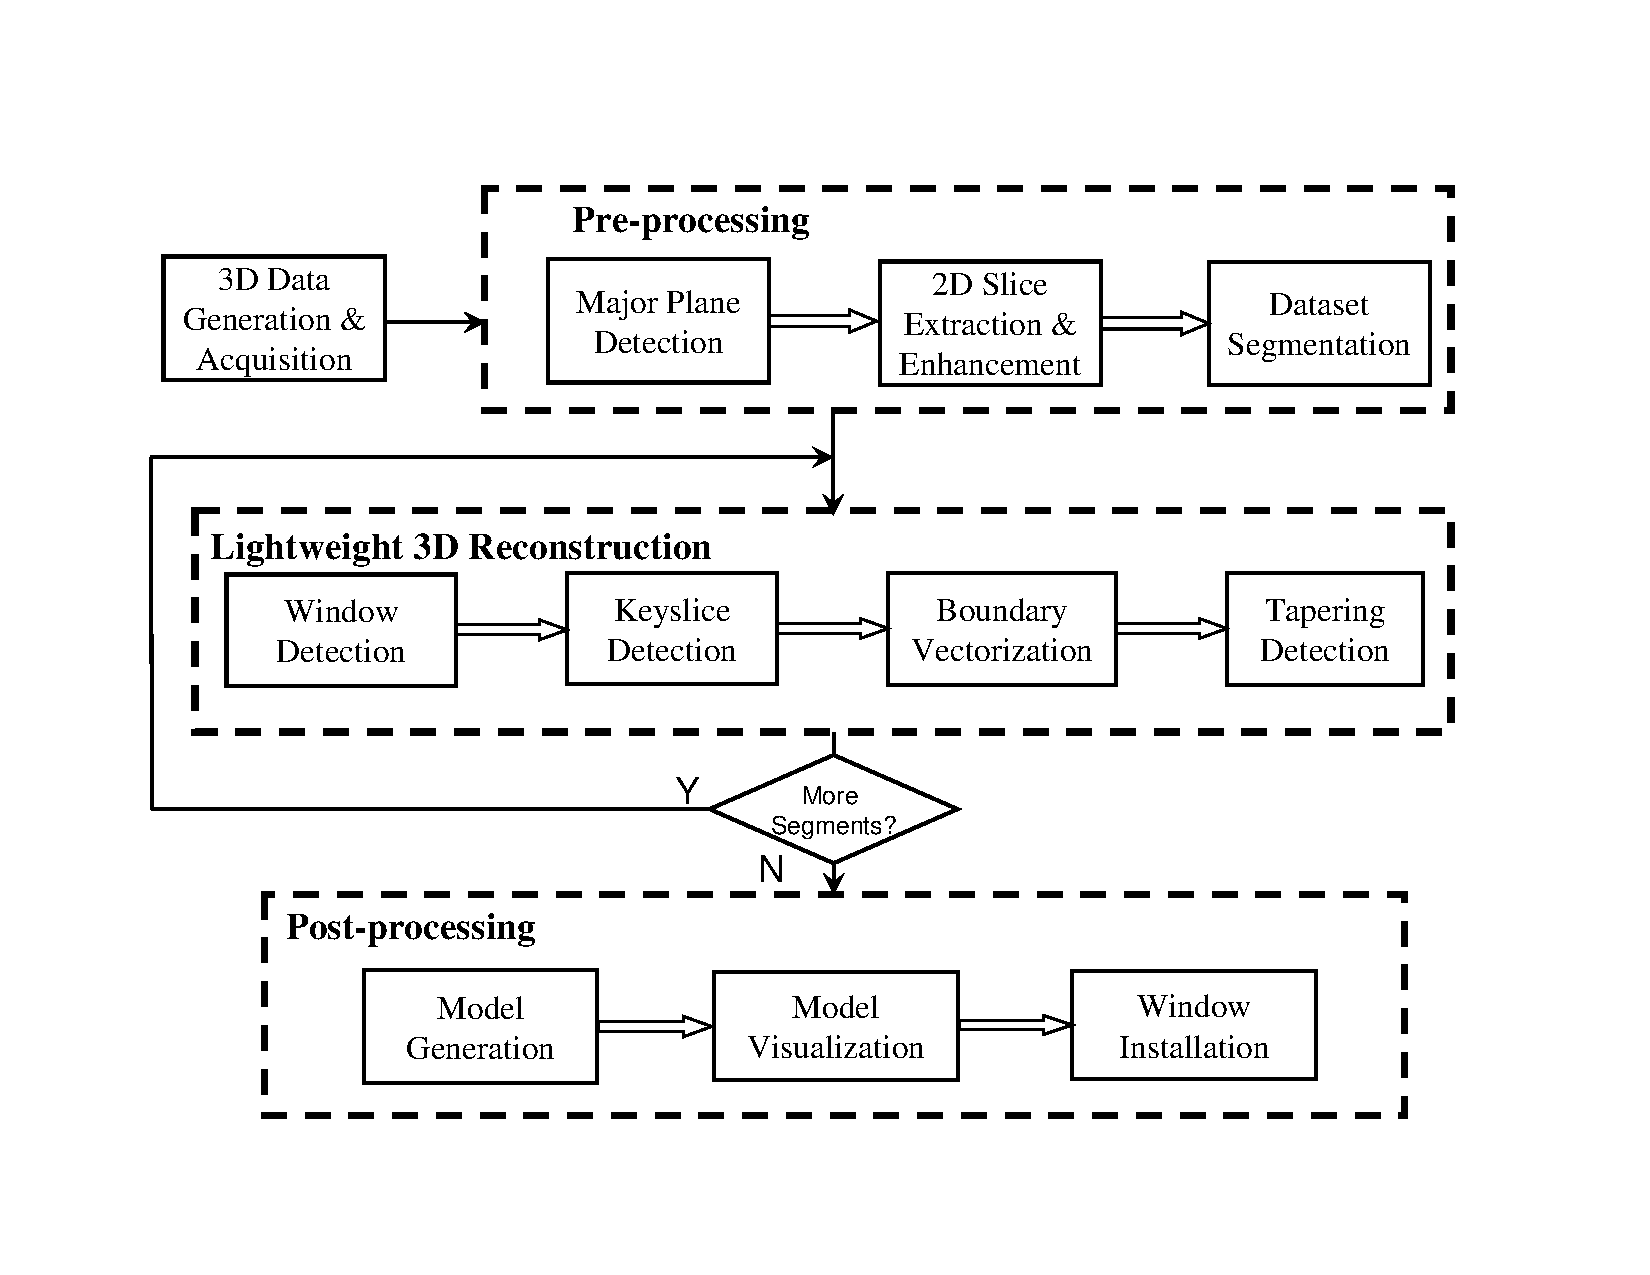
\includegraphics[width=\textwidth]{flow.pdf}
      \caption{Flow graph for proposed approach}
      \label{fig:flow}
\end{figure}

An overview of our approach, depicted in \Fig{ov}, begins with the
acquisition of a dense 3D point cloud $C$ of a building.
$C$ is then partitioned into a nonoverlapping set of volumetric slabs.
Each slab $S$ is associated with one projection plane $P$,
sitting at the base of $S$.
The purpose of partitioning $C$ is to establish a set of cross-sections,
or contour slices.
By examining the changes among these slices, we can identify the prominent
slices, or {\it keyslices}, as well as the necessary extrusion and
taper operations that must apply to them to generate the model.
By casting this 3D modeling task into a series of 2D operations, we
reduce the dimension of the problem to achieve a significant savings in
computational complexity.

To generate the 3D model of a building, all these key raster images need 
to be vectorized to represent the silhouette or boundary of the building. 
Couple of raster image vectorization approaches are
proposed in \cite{DP_AAKMT, DP_DP, DP_WM}. The Douglas-Peucker
algorithm tried to connect all the existed points to form a polygon. 
Although the implementation of
this approach is very efficient with the improvement in \cite{DP_HS},  this method cannot
handle the case where some extra interior points are existed as some outlier data.
To tackle this issue, Medeiros et al. \cite{BPA_MVL} applied ball-pivot algorithm (BPA)
\cite{BPA_BMRS}, which was original proposed on 3D point cloud data, on the 2D image to obtain
vectorized boundary. The key parameter for BPA to work successfully is to find the right size of
the ball for pivoting. We have proposed an adaptive BPA algorithm to solve this problem.

\begin{figure}[htbp]
\begin{center}
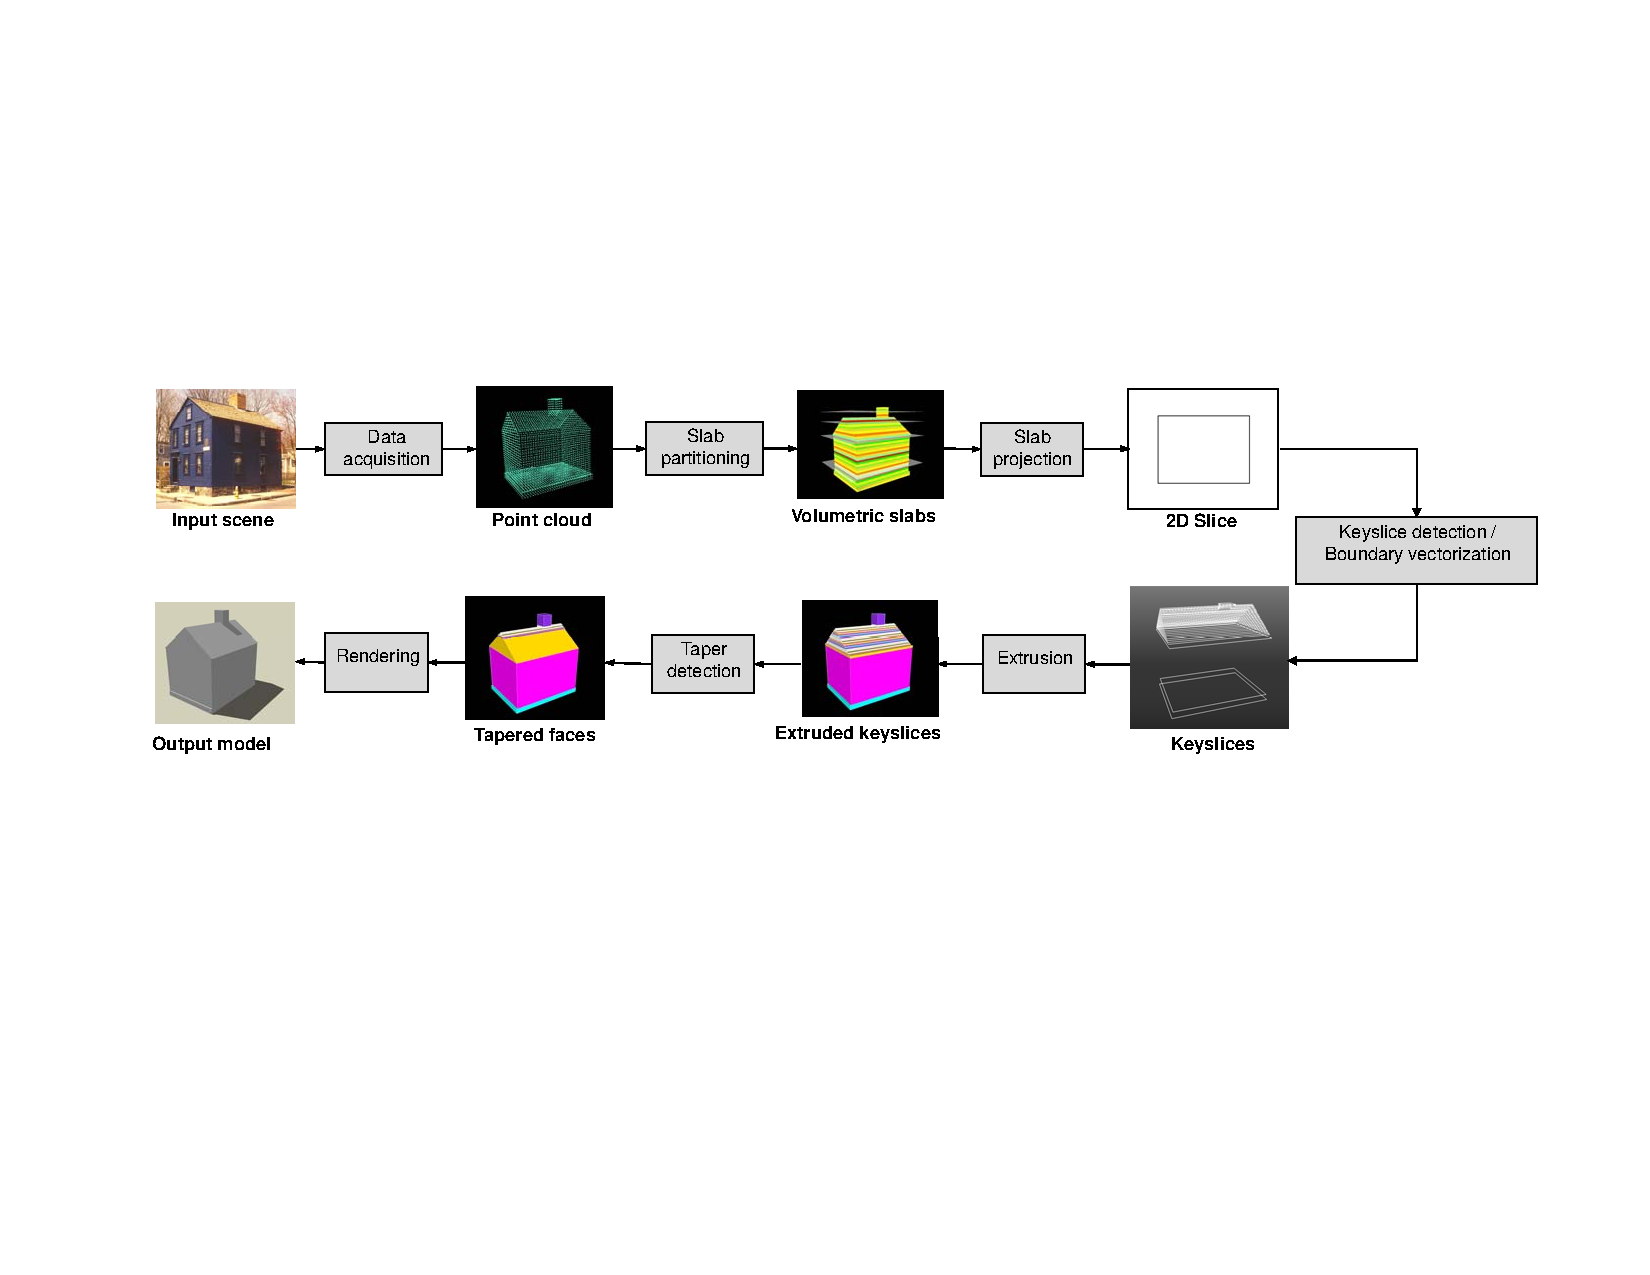
\includegraphics[width=1.0\textwidth]{overview.pdf}
\end{center}
\caption{Overview of the proposed approach.}
\label{fig:ov}
\end{figure}

Due to occlusion and material-dependent reflection problems off of glass
(e.g., windows), the input data is incomplete and noisy.
Therefore, noise removal and hole filling are carried out as a
preprocessing stage to generate the 3D model.
The next stage of the approach is to carry out fast image processing
techniques on the enhanced image slices to detect keyslices.
Boundary vectorization for these raster keyslices is then conducted to
transform these points into polygons.
Tapered structure detection is carried out to further reduce the model size.
Finally, 3D model generation is achieved by applying the extrusion/taper
operations to the keyslices to reconstruct lightweight 3D models of urban
buildings from range data.

\newchapt{Preprocessing on Range Data}{chapt2}{Preprocessing on Range Data}

%%%%%%%%%%%%%%%%%%%%%%%%%%%%%%%%
%%%%%%   PREPROCESSING  %%%%%%%%
%%%%%%%%%%%%%%%%%%%%%%%%%%%%%%%%
%\section{Preprocessing the Range Data}
\label{sec:prep}

The input to our system is range data assembled as a 3D point cloud.
Our data is obtained from a Leica Cyrax 2500 laser range scanner \cite{RDP_LRS},
which works by sweeping an eye-safe laser beam across the scene to collect
up to one million 3D depth points per frame.
All scene points that lie within 100 meters can be acquired with an accuracy
of 5mm in depth.
The basic algorithm that we use for registering the voluminous 3D data
acquired from multiple scans of buildings has been introduced in
\cite{RDP_LS}.
That same algorithm is also responsible for extracting the major axes
of the building in order to align it to the axes of the world coordinate
system.
This is necessary to properly infer the keyslices.
\Figb{IR_2_DXF} displays a properly aligned, {\it registered} 3D point cloud
consisting of 14 scans totalling 14 million points.

\begin{figure}[htbp]
\begin{center}
\begin{tabular}{c}
	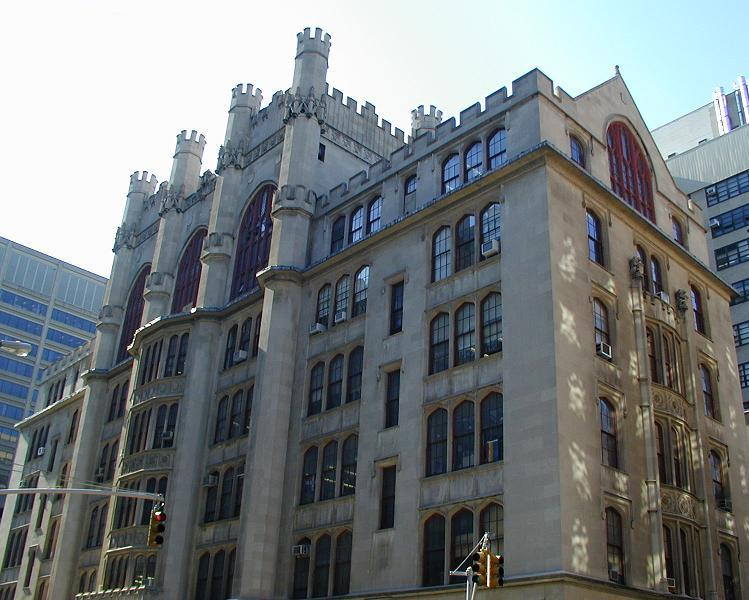
\includegraphics[width=0.6\textwidth]{HunterPhoto.jpg} \\
	(a)\\
	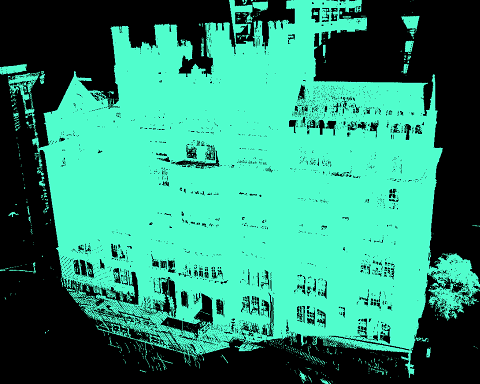
\includegraphics[width=0.6\textwidth]{point_cloud.png} \\
	(b)
\end{tabular}
\end{center}
\caption{
(a) Image of building to be modeled.
(b) 3D point cloud of building assembled by registering multiple scans.
}
\label{fig:IR_2_DXF}
\end{figure}

Due to occlusions and limited vantage points, the point cloud collected by the
laser scanner contains artifacts and holes.
In addition, computing directly on 3D data is time-consuming and
computationally complex.
To tackle these issues, we define inner and outer bounding boxes for the
building to clip away unrelated scene objects.
Then, we convert the 3D modeling problem into a set of 2D problems by
projecting the 3D data into a series of 2D cross-sectional contour images.
Noise removal, hole filling, and vectorization are all done in this
2D space.

%%%%%%%%%%%%%%%%%%%%%%%%%%%%%%%%
%%%%%% 3D Data Rectification %%%
%%%%%%%%%%%%%%%%%%%%%%%%%%%%%%%%
\section{Point Cloud Rectification}
\label{sec:rect}

%% Put the flow of the data rectification.
Although the multiple scans of point cloud data have been registered, 
they are not rectified as depicted in \Fig{pc_orig}. 
Please note the point cloud has been sub-sampling by a factor of 50.
This is not suitable for our further 3D modeling.
As one of the pre-processing steps, this registered data will be rotated
and translated to be aligned with world coordinates.

%% Put the image of rectfied data.
\begin{figure}[htbp]
\begin{center}
\begin{tabular}{c}
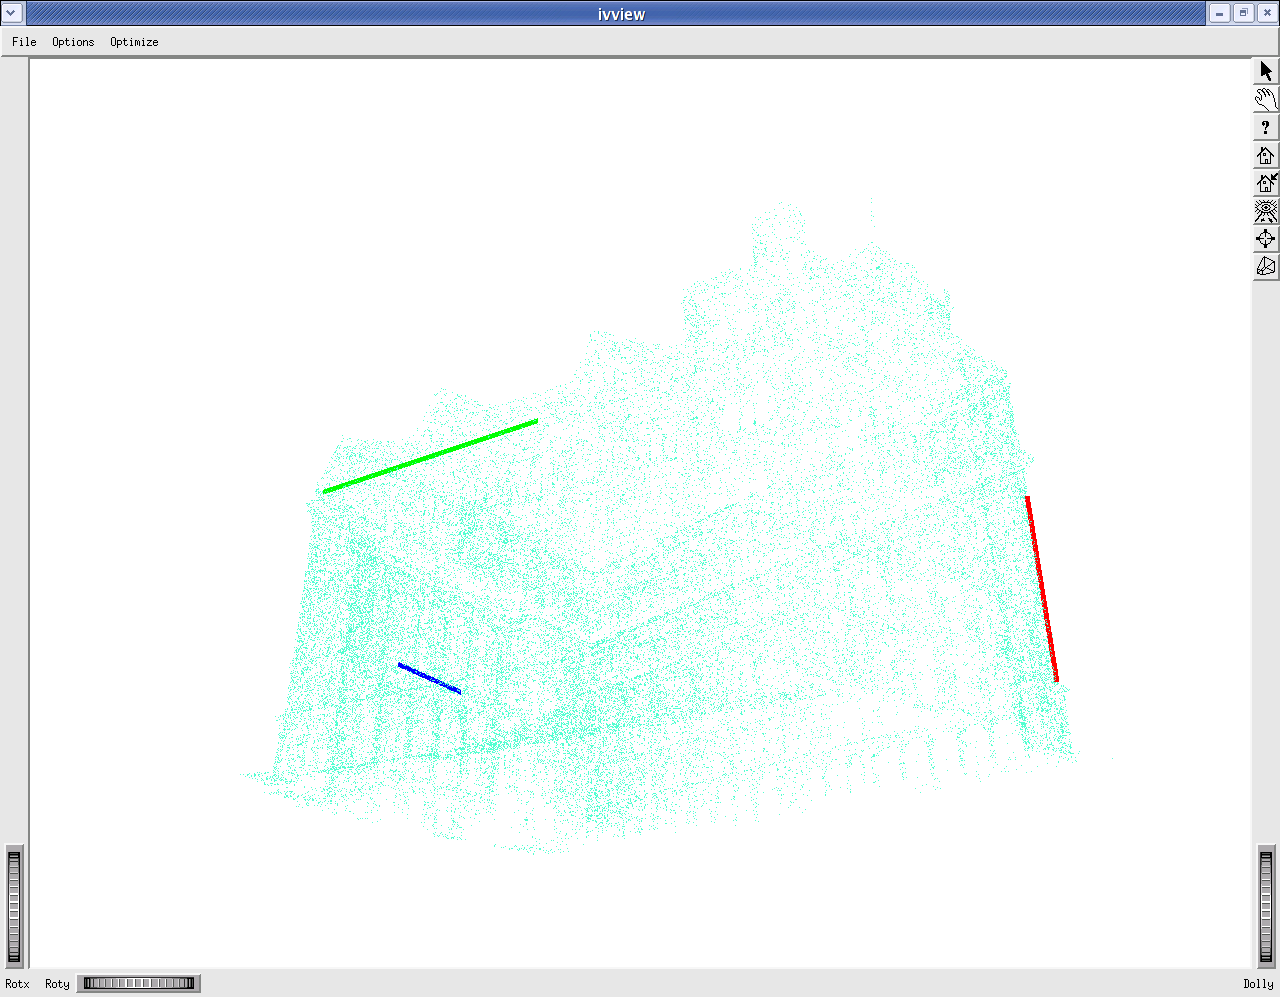
\includegraphics[width=\textwidth]{point_cloud_not_rect.png}
\end{tabular}
\end{center}
\caption{ The registered point cloud without rectification. }
\label{fig:pc_orig}
\end{figure}

As we know, there are a lot of line features existed in the point cloud, which
provides a good clue for rectifying the data. 
For each scan $s$ of the scene, we can obtain a set of line segments $L_s$. 
Assume $T_s$ is the transformation matrix for the scan $s$ to be registered with other scans.
In other words, for any point $P(x,y,z)$ in the scan $s$, $P*T_s$ will transform the
point $P$ into the final registered coordinate system as shown in \Fig{pc_orig}.

We can obtain the major axises by clustering these line segments $L_s$ from different
scans. The purpose of clustering is to group the lines whose direction are very close to each other.
To cluster these lines, we first transform the line segments in $L_s$ into world
coordinate system using $T_s$ as described above. After transformation, we will
get a larger line set $L = {l_1, l_2, \ldots, l_n}$. For each line $l_i$, we first
normalize it to a unit vector:
\begin{equation*}
\overline{l_i} = \frac{l_i}{\parallel l_i \parallel}
%% \bar --> \overline
\end{equation*}

The unit vector $\overline{l_i}$ has the unique length 1, which provides a good starting point 
for clustering since we do not need to worry about the length of the lines. 
An array of bins are used to hold the unit vectors.
As the initial step, the first line $\overline{l}$ is picked up and is insert into the 
first bin and set the counter of the bin to 1.
When a new unit vector $\overline{l_n}$ is observed, we try to see whether there is an
existed unit vector in the bins which has similar direction as $\overline{l_n}$. This is
done by computing the distance $d_{\pm}=\parallel \pm\overline{l_n} - \overline{l_i} \parallel$.
Because $\overline{l_n}$ can has two opposite directions, we can compute both of them and
choose the smaller value as the distance $d$. If $d$ is smaller enough, $\overline{l_n}$
is clustered with the line $\overline{l_i}$ and the counter of the bin holding $\overline{l_i}$
is increased by 1. On the other hand, if $d$ is big, we have to compare $\overline{l_n}$
with a line in the next bin. If $\overline{l_n}$ could not fit any line in the bins, we
will insert $\overline{l_n}$ into a new bin and set the counter of the bin to 1. 
To avoid the bias of the initial select, each unit vector $\overline{l_i}$ is
adjusted to be the mean of all unit vectors falling inside this bin. 

Once we go through all the lines in $L$, the clustering is complete. 
The next step is to choose the major axises from the clustering results. 
Essentially, this is to choose bins whose counters are among largest. 
Assume $u$, $v$, and $n$ represent the three largest bins. This is demonstrated in
\Fig{pc_orig} in red, green and blue respectively. To rectify the data,
we can refer to the following transformation matrix $\mathbf{M}$:
\begin{figure}[htbp]
\begin{center}
\begin{tabular}{c}
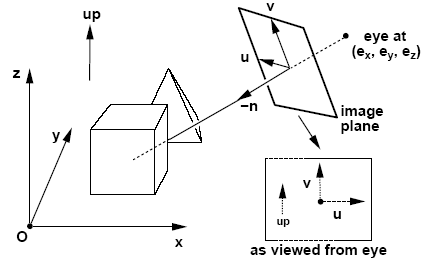
\includegraphics[width=0.5\textwidth]{point_cloud_rect_matrix.png}
\end{tabular}
\end{center}
\caption{ The transformation matrix. }
\label{fig:pc_rect_matrix}
\end{figure}

\begin{equation*}
\mathbf{M} = \left(
\begin{array}{cccc}
u_x & u_y & u_z & -e_x \\
v_x & v_y & v_z & -e_y \\
n_x & n_y & n_z & -e_z \\
  0 &   0 &   0 &    1 
\end{array} \right)
\end{equation*}

This is illustrated in \Fig{pc_rect_matrix}. $(x, y, z)$ is the world coordinate system.
The rectified coordinate system is represented using $(u, v, n)$. 
The vector $[-e_x, -e_y, -e_z]^T$ is the translation of the view point from the world origin.
After the transformation with $\mathbf{M}$, the new data set and the three major line segments are
shown in \Fig{pc_rect}.

%% rectified data
\begin{figure}[htbp]
\begin{center}
\begin{tabular}{c}
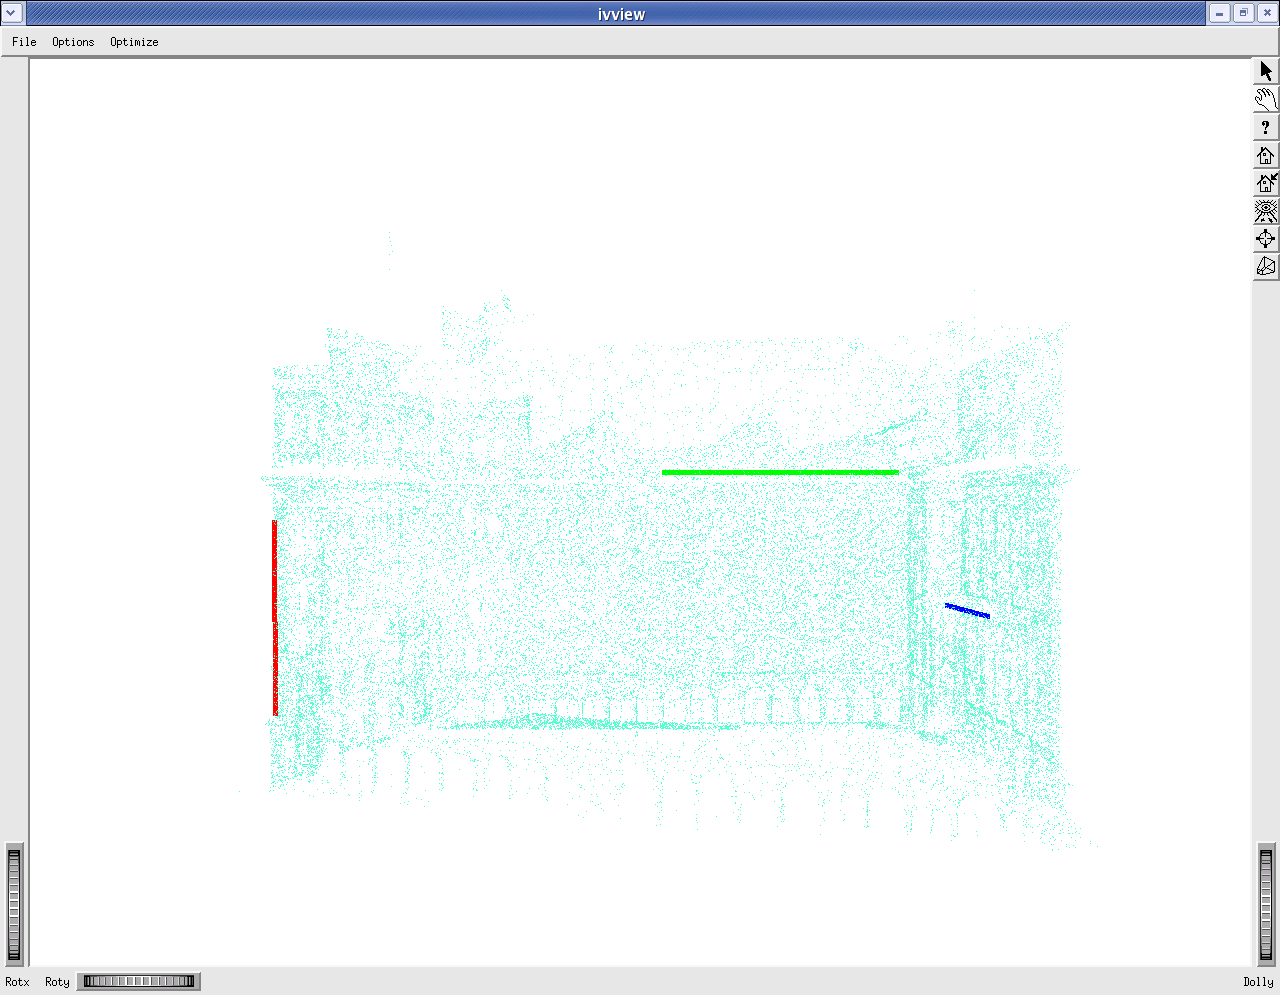
\includegraphics[width=\textwidth]{point_cloud_rectified.png}
\end{tabular}
\end{center}
\caption{ The rectified point cloud of \Fig{pc_orig}. }
\label{fig:pc_rect}
\end{figure}


\section{Extraction of 2D Slices}
\label{sec:image_slicing}

We consider the point cloud data as a large array of 3D points to be
sliced into horizontal volumetric slabs.
All 3D points within each slab are projected onto a horizontal projection
plane, or slice, at the base of the slab.
\Fig{slice_slab} shows the 3D point cloud in \Figb{IR_2_DXF} partitioned into
50 slabs.
The 3D points in each slab are projected onto a projection plane to
form cross-sectional contour slices.
\Fig{slicing} depicts four such slices, associated with the four displayed
projection planes of \Fig{slice_slab}.

\begin{figure} [htbp]
\begin{center}
\begin{tabular}{c}
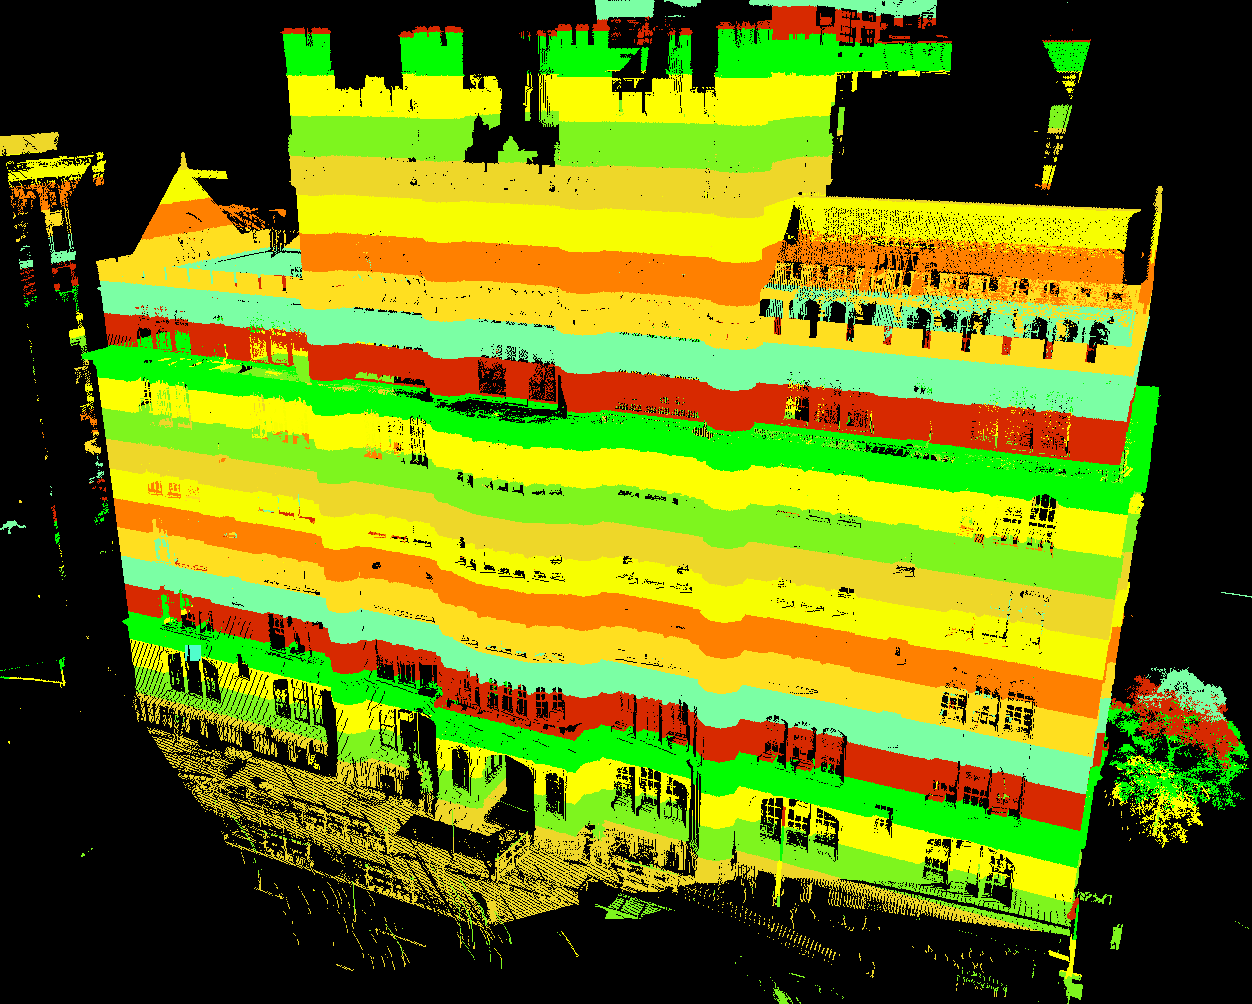
\includegraphics[width=0.6\textwidth]{slab_noplanar.png} \\
(a) \\
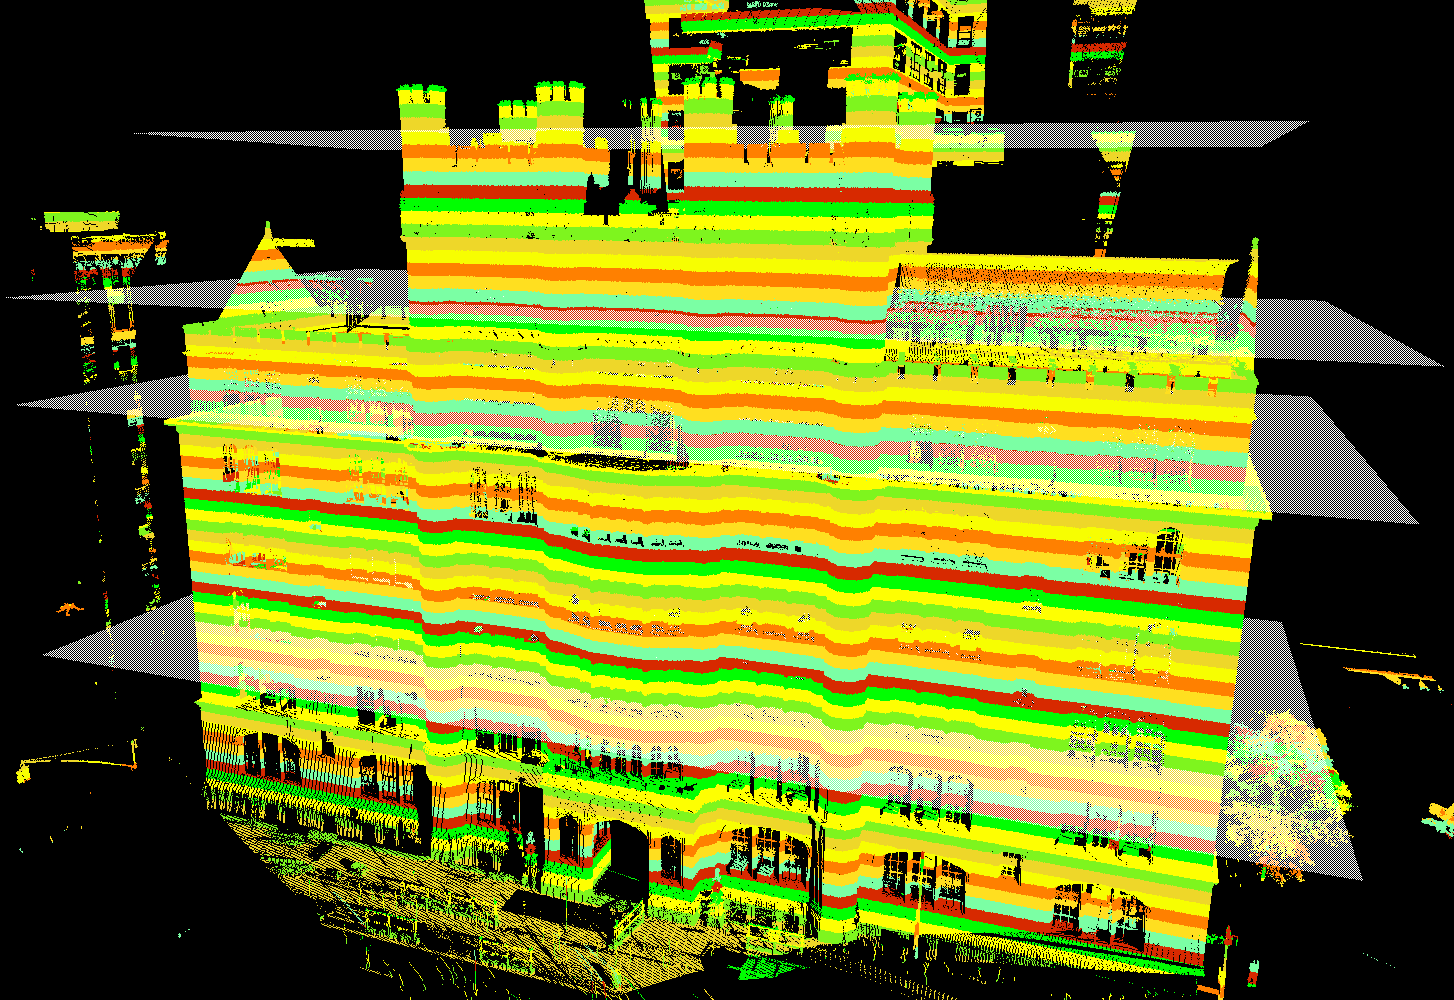
\includegraphics[width=0.6\textwidth]{slab_planar.png} \\
(b)
\end{tabular}
\end{center}
\caption{
(a) Slabs of the 3D point cloud data are used to determine prominent
cross-sections upon which extrusion/taper operations are applied.
(b)The 3D point cloud of \Figb{IR_2_DXF} partitioned into uniform
volumetric slabs.
The 3D points in each slab are projected onto a projection plane to
form cross-sectional slices. Four such planes are shown.}
\label{fig:slice_slab}
\end{figure}

The height of each slab is $\boldsymbol{\delta}$.
If $\boldsymbol{\delta}$ is held constant, each slice is generated from
equi-spaced slab intervals.
If $\boldsymbol{\delta}$ is allowed to vary, then we may
choose to allow for large values in parts of the structure that are similar,
and low values in regions that contain finer detail.
To avoid working on 3D data directly, a relatively small constant value
for $\boldsymbol{\delta}$ is chosen to generate 2D cross-sectional image slices.

\begin{figure} [htbp]
\begin{center}
\begin{tabular}{cc}
\fbox{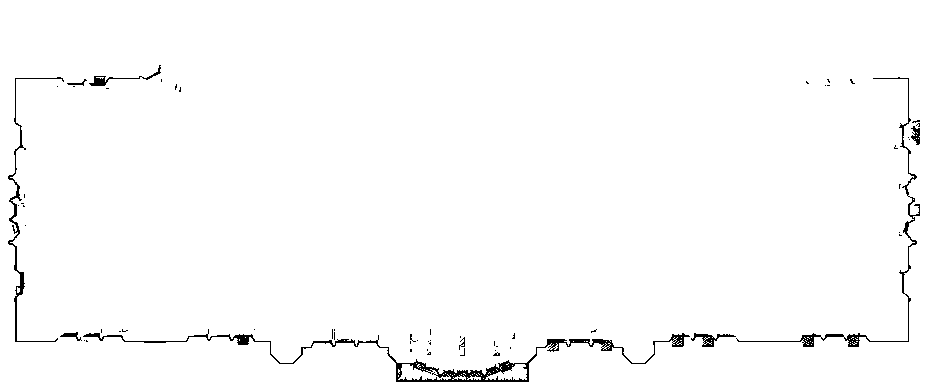
\includegraphics[width=0.45\textwidth]{image_slice_0190.png}} &
\fbox{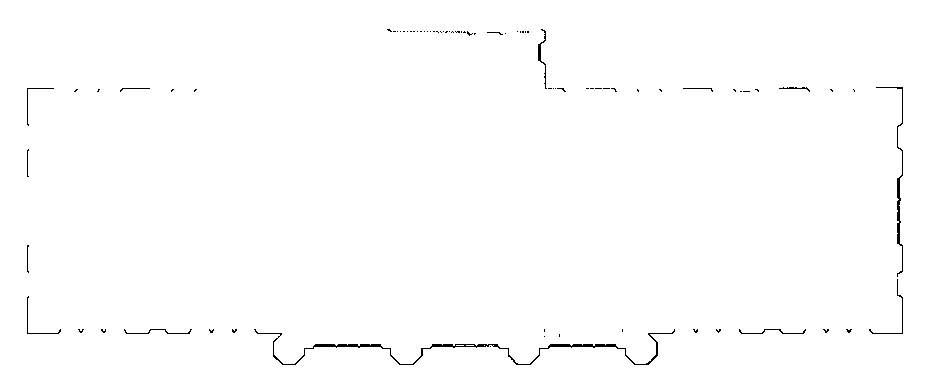
\includegraphics[width=0.45\textwidth]{image_slice_0600.png}} \\
(a) & (b) \\
\fbox{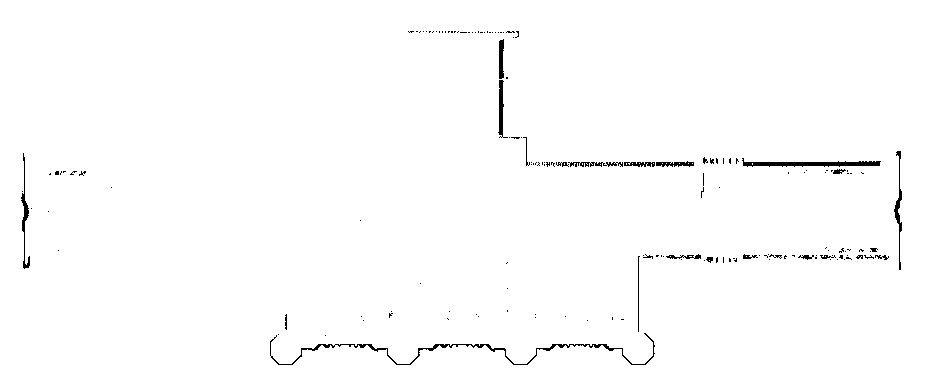
\includegraphics[width=0.45\textwidth]{image_slice_0714.png}} &
\fbox{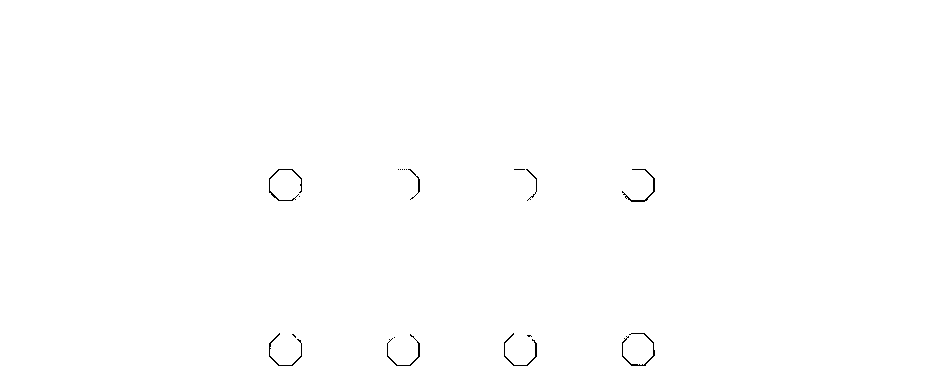
\includegraphics[width=0.45\textwidth]{image_slice_0951.png}} \\
(c) & (d)
\end{tabular}
\end{center}
\caption{The set of slices corresponding to the four projection planes in
\Fig{slice_slab}.}
\label{fig:slicing}
\end{figure}

Without loss of generality, the $y-$axis is used to represent the bottom-up
vertical direction.
Over each slab in height range $[H_{lo}, H_{hi})$,
we project the 3D data $\boldsymbol{P}(x,y,z)$, for $H_{lo} \leq y < H_{hi}$,
onto a 2D image slice.
The projection is normalized in the range $[0,W]$, where $W$ is the image width:
\begin{equation}
[\,x^{2D},\; y^{2D}\,]^T = \omega\cdot[\,x^{3D}_i - X_{MIN},\; z^{3D}_i - Z_{MIN}\,]^T
\label{eq:image_slicing}
\end{equation}
Note that $\omega = W/(X_{MAX} - X_{MIN})$, and that
the [$X_{MIN}$, $X_{MAX}$] and [$Z_{MIN}$, $Z_{MAX}$] pairs define the
3D bounding box, which can be obtained through user input and can be used
to clip away noise data.
\Fig{slicing}(a)-(d) show some examples of the 2D slices, where noise
and incomplete data are observed.

\newchapt{Slice Enhancement}{chapt3}{Slice Enhancement}

%%%%%%%%%%%%%%%%%%%%%%%%%%%%%%%%
%%%%%%   Slice Enhancement  %%%%
%%%%%%%%%%%%%%%%%%%%%%%%%%%%%%%%
\section{Hole Filling}
\label{sec:mdr}

The slices we extract above often have holes (i.e., missing data) due to
occlusion or other visibility issues.
Fortunately, most urban buildings have symmetry that we can exploit to
fill these holes.
Symmetry computation on 3D data is an active research topic, such as those in
\cite{Sym_PSGRF,Sym_ZPA,Sym_TW,Sym_MGP}, which has potentially numerous applications.
However, symmetry computation 3D data directly is expensive. 
Here, we only conduct this computation on the 2D image slices.
Since the 3D data has been already rectified \cite{RDP_LSYGS} 
and projected onto 2D slices, hence only 2D translation
is needed to be considered for symmetry computation.
Let $P(x,y)$ be a point on the original image $I$ and $P'(x',y')$ be the reflected
point of $P$ with respect to a symmetry line $L$.
The symmetry computation equation for $L$ is as follows:
\begin{equation}
L = \underset{x,y}{\operatorname{arg\,min}}\sum{d_{x,y}(P', I)}
\end{equation}
where the $d_{x,y}(P',I)$ is the distance between the self-reflected point
$P'$ and its nearest data point in image $I$.
The reflected point $P'$ of the original point $P$ is computed with
respect to a line along either the $x-$ or $y-$ axis.
Therefore, the symmetry line $L$ is obtained as the line with minimum
summation error over the reflected data points.
\Figa{sym} and \Figb{sym} depict the original input with holes, and
the output after hole filling using symmetry computation, respectively.

\begin{figure}[htbp]
\begin{center}
\begin{tabular}{c}
\fbox{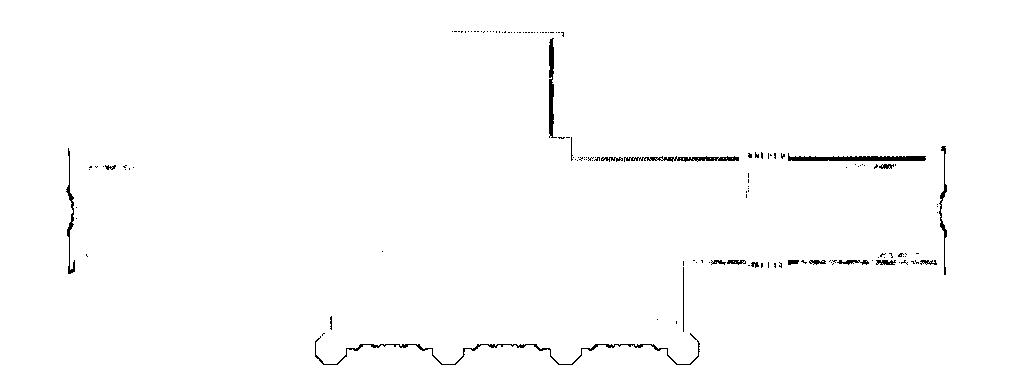
\includegraphics[width=0.6\textwidth]{image_slice_0705_0711.png}} \\
(a) \\
\fbox{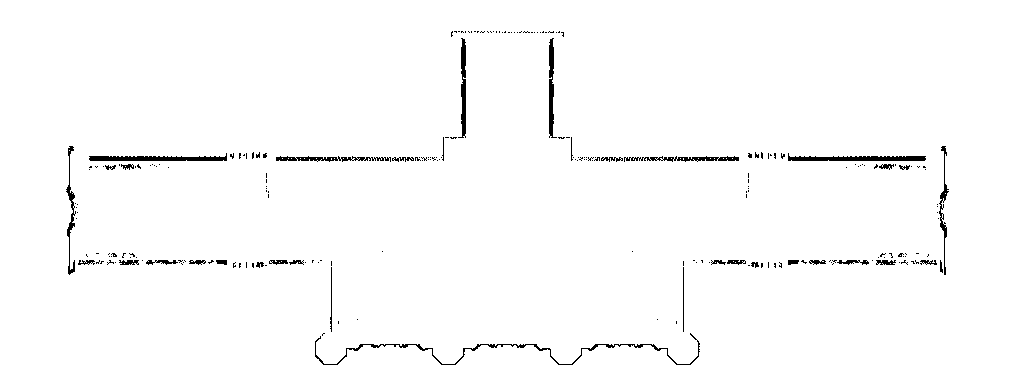
\includegraphics[width=0.6\textwidth]{image_slice_0705_0711_recoverd.png}} \\
(b)
\end{tabular}
\end{center}
\caption{ Symmetry-based hole filling. (a) Original 2D slice image and
(b) output image after hole filling.}
\label{fig:sym}
\end{figure}

\newchapt{Keyslice Detection}{chapt4}{Keyslice Detection}

%%%%%%%%%%%%%%%%%%%%%%%%%%%%%%%%
%%%%%%   3D Reconstruction  %%%%
%%%%%%%%%%%%%%%%%%%%%%%%%%%%%%%%
%\section{Lightweight 3D Reconstruction}
\label{sec:reconst}
Our 3D modeling algorithm is based on \emph{a priori} knowledge that
urban buildings can be created through a series of extrusion and taper
operations on the salient cross-sections contained in the keyslices.
\Fig{keyslices} depicts the keyslices derived from the uniform slices
given in \Fig{slice_slab}. 
The key step for successful modeling is identifying these salient cross
sections upon which the extrusion and taper operations will apply.

An intuitive way for key slice detection is to 
compute the similarity between the sliced images.
In other words, the sliced images are clustered into different groups 
based on the similarity among them.
There are two mainly research methods for similarity measurement of 2D images: 
area based method and feature based methods. 
The area based methods are computational efficient 
but they usually can only be applied on binary or gray-scale images. 
The feature based one is computational complex but more powerful 
and can be applied to images obtained using different sensors, 
such as multi-modal image registration.
% read similarity measure papers.
Because our goal is to develop light-weight efficient algorithm for model reconstruction, 
plus the input for similarity measure is pure binary images, 
the area based method is adopted for our approach.

The classical measurement for area based method is the normalized cross
correlation \cite{DIP_Pratt}:
\begin{equation*}
CC(i,j) = \frac{\sum_W(W - E(W))(I_{(i,j)}-E(I_{(i,j)}))}
{\sqrt{\sum_W(W - E(W))^2}\sqrt{\sum_{I_{(i,j)}}(I_{(i,j)} - E(I_{(i,j)}))^2}}
\end{equation*}
where $W$ is an image mask, $E(W)$ is the mean of the mask's pixels, 
and $E(I_{(i,j)})$ is the mean of the image pixels covered by the mask $W$.
However, this method is very time consuming and is a local window-based approach,
which could not capture the global relations between images. 
Therefore, we proposed a light-weighted global and efficient key image detection approach 
based on Hausdorff distance and curvatures computation.

\begin{figure}[hbtp]
\centering
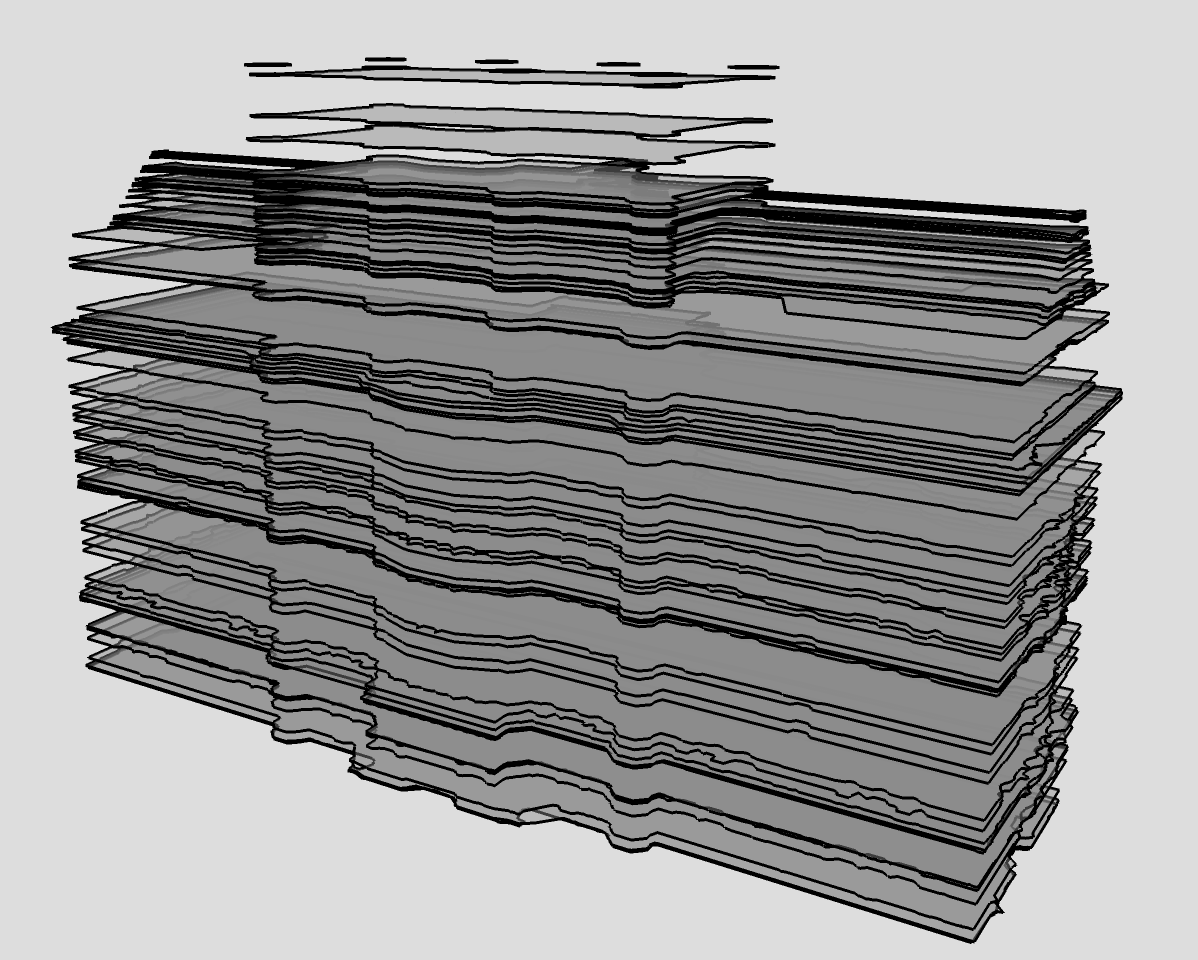
\includegraphics[width=0.8\textwidth]{figures/keyslice_wireframe.png}
\caption{Keyslices derived from the input in \Fig{slice_slab}.}
\label{fig:keyslices}
\end{figure}

\section{Hausdorff Distance Based}
\label{sec:ksd}
The 2D image slices of an extruded region are similar to each other.
Thus, to detect the keyslices that delimit extruded regions one only needs
to compute the similarity between adjacent slices.
We select the Hausdorff distance \cite{IR_HKR} as the similarity measurement.
Let $P_r(x_r, y_r)$ be a data point in a reference image and
let $P_i(x_i, y_i)$ be a data point in a new observed image $I$.
The Hausdorff distance of image $I$ to reference image $I_r$ is defined as:

\begin{equation}
d_H(I, I_r) = \sum_{i=0}^Nd_{min}(P_i, I_r)
\label{eq:hd}
\end{equation}

where $d_{min}(P_i, I_r)$ is the minimum distance from data point $P_i$
in image $I$ to the reference image $I_r$.
Alternatively, we can also define the Hausdorff distance, $d_H(I_r, I)$,
from reference image $I_r$ to a new observed image $I$, using \Eq{hd}.
These two distances are usually not equal to each other.
As a rule of thumb, one can choose
$d_{HD} = \text{MAX}\{d_H(I, I_r), d_H(I_r, I)\}$ as the Hausdorff distance.
To compute the keyslices, a threshold $\tau_{d}$ is used for the
Hausdorff distance $d_{HD}$.
If $d_{HD} < \tau_{d}$, the two images $I$ and $I_r$ are considered
similar to each other.
Otherwise, a keyslice image is found and $I_r$ is updated with $I$,
the new keyslice image.

\section{Curvature Based}
The accuracy of the keyslices detected by using the Hausdorff distance
is closely tied to threshold $\tau_d$.
Small $\tau_d$ leads to more accurate models and will require more time and
space to compute and store the result.
When the threshold $\tau_d$ is relatively large, potential keyslices which
contain salient structure may be missed.
Therefore, there is a trade-off between model accuracy and time-space
efficiency.
To address this problem, the curvature information is computed as a
complementary criteria for keyslice detection.

This idea is based on the observation that the keyslices are generally
located at large curvature changes along 2D slices extracted in the orthogonal
direction (e.g., side view), as shown in \Figa{HT_BPA_Curvature}.
Therefore, instead of computing the difference between two images directly,
we compute the curvature of orthogonal 2D slices, map the positions of
curvature extrema back to cross-sections in the original set of volumetric
slabs, and mark these cross-sections as keyslices.

\begin{figure}[htbp]
\begin{center}
\begin{tabular}{cc}
\fbox{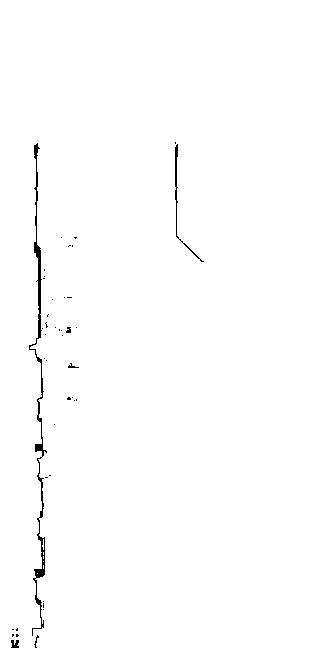
\includegraphics[width=0.3\textwidth]{image_slice_lr_0580_0590_half.jpg}}
\fbox{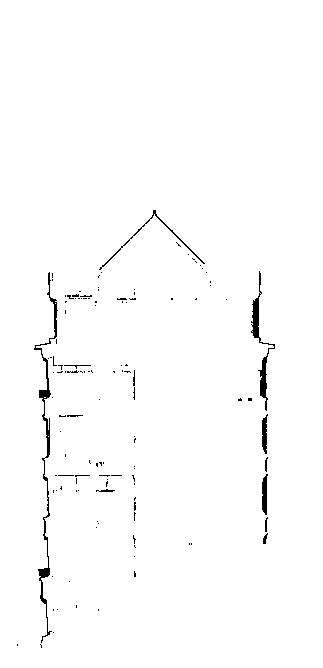
\includegraphics[width=0.3\textwidth]{image_slice_lr_0830_0842_half.jpg}} &
\fbox{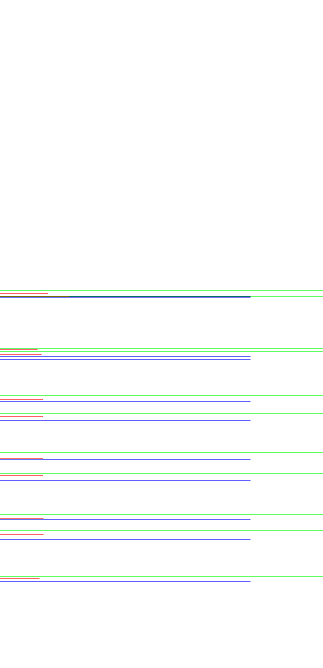
\includegraphics[width=0.3\textwidth]{curvature_center_lines_old_half.jpg}} \\
(a) & (b)
\end{tabular}
\end{center}
\caption{Curvature-based key slice detection.
(a) A partial set of two 2D sliced images from the orthogonal direction (side
view). The complete set will be used to extract the keyslices shown in
\Fig{keyslices}.
(b) The average curvatures detected over all of the sliced images along the
orthogonal direction.}
\label{fig:HT_BPA_Curvature}
\end{figure}

In the close-up view of a small region as shown in \Fig{KSD_Curv},
two curvatures, $c_1$ and $c_2$, are
computed in this small region. The red, blue and green lines indicate the locations
of the center, the starting and the ending of a curvature. 
As a matter of fact, there is a third curvature computed around the
black box sitting on top of the green line of the curvature $c_1$. 
However, this third one should not be consider as a real curvature 
in that the black box is due to an air conditioner during the data acquisition process, 
which means it is not a part of the building. We called this third curvature
{\it outlier curvature} which needs to be removed from the set of real curvatures.
Based on the fact that these outlier curvatures exist only in a few 2D slices,
we can exclude them by counting the number of appearance for each curvature.
Only those curvatures appears in most of the 2D slices are kept for further computation.

Once the real curvatures are obtained, they can be used as a complemental way of 
Hausdorff distance for keyslices detection. 
Each curvature $c$ is mapped to a set $s$ of original 2D cross-sectional
slices, $i,\ldots,j$, where $i$ and $j$ are corresponding to the starting and 
the ending locations of $c$. After this, the set $s$ is checked whether 
it contains any keyslice or not.
If a keyslice $k$ has been marked in $s$ by Hausdorff distance, 
nothing needs to be done and this curvature $c$ is discarded. 
On the other hand, if $s$ contains no keyslice, $i$ and $j$ will be marked as 
two new keyslices to keep the salient feature identified by this curvature $c$.
The combination of Hausdorff distance measurement and curvature inference
ensures that the salient structures of a building will be preserved.

%%% Figure of the tapered template.
\begin{figure}[htbp]
\begin{center}
\begin{tabular}{c}
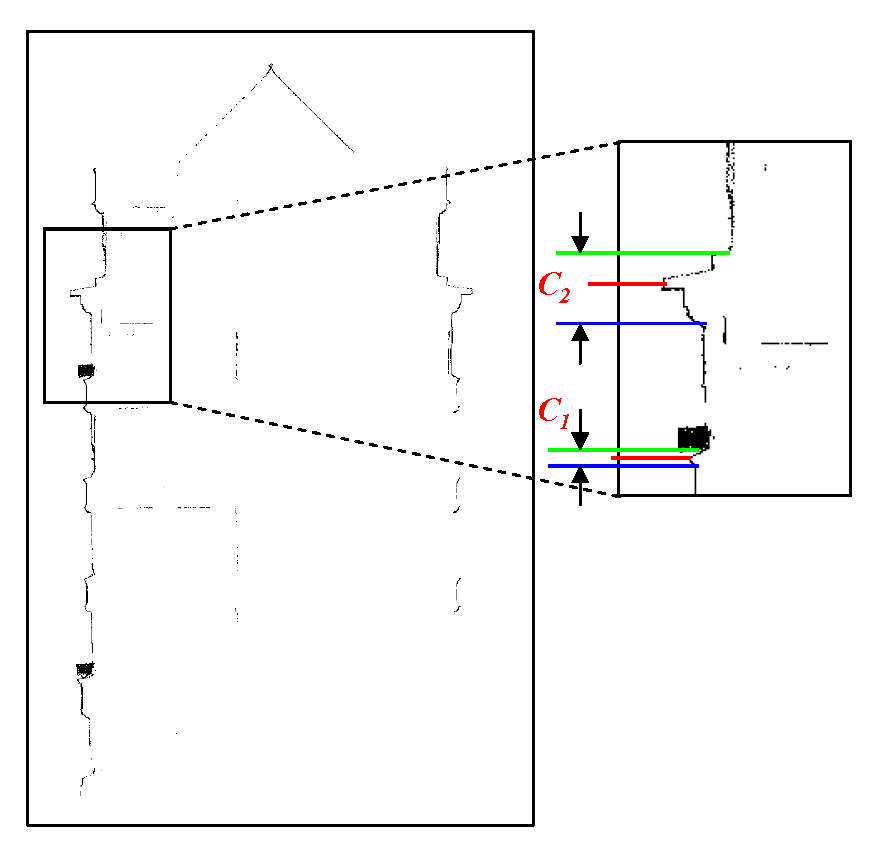
\includegraphics[width=0.60\textwidth]{curvature.png}
\end{tabular}
\end{center}
\caption{ Curvature based key slice detection. }
\label{fig:KSD_Curv}
\end{figure}
%%% End of Figure

To compute the curvature, we first apply the slice extraction algorithm
described in \Sec{image_slicing} to obtain a series of 2D cross-sectional
images in the orthogonal direction.
We then apply the ball-pivot algorithm described in \Sec{BPA} to
vectorize the boundary for each sliced image.
We locate those curvatures that appear in most of the sliced images as the
places where keyslices are found, as shown in \Figb{HT_BPA_Curvature}.
Note that the red lines indicate location of the center of the curvature,
and the blue and green lines indicate the entering and exiting of the
curvature structures, respectively.
The combination of Hausdorff distance measurement and curvature inference
ensures that the salient structures of a building will be preserved.

\section{Local Matching Based on Segmentation}

The keyslice detection described above are based on global information matching.
The strength of these methods lies on the effective of computation and they can
also produce good results on exterior scanning as depicted in %\Fig{keyslices}. 
However, when applied to interior scannings when the layout of the structures 
is complex, there may be some limitations on these methods. 
As depicted in %\Fig{ksd_gbl_bad}, the pillars inside the hall can be reconstructed
by simple extrusion of the base polygon. However, they are divided to 
excessive amount of keyslices because the dissimilarity of the outside window
structures in the same projection level. In other words, due to global matching
strategy, some independent objects which could be modeled using simple extrusion
operation are modeling using excessive keyslices. Although the reconstructed
models are still correct at this situation, they are not efficiency. That is, much
more keyslices are created to represent the simpled extruded parts. 

A more effective way for modeling the above structures is to model the different 
structures individually. By doing this, we can simply model the pillars using a
extrusion operation based on a base polygon. Certainly, for the complicate window
structures, more keyslices are still required but these keyslices would not contain
any pillar structures. To do this, segmentation is a necessary step to identify
all different parts of the scannings. 

There are a lot of literatures on image segmentation as in %\cite{segmentation}. 
% a little bit survey on image segmentation, especially binary image segmentation.
% why the graph-cut is well-fit for our purpose.

Our segmentation based keyslice detection approach is an iterative algorithm.
We first applied the graph cut
on the 2D sliced binary image. The initial input to graph cut is done as follows. 
First of all, a random data point $p$ was located in the binary image $I$. The data
point $p$ is then growing to form an region $r$ based on the connected components 
until it reaches a fix-point. That is, no more data point can be reached in $r$. $r$
is taken as input by graph cut algorithm to compute the segmentations. 
The segmented objects (non-background pixels) are then stored and their pixels are 
reset to background pixels for next iteration. The algorithm is depicted in %\Fig{alg_seg}.
To adjust the accuracy of the graph cut, the parameter ??? was used. To get more
accurate segments, which means more objects may be classified, enlarge/shrink its value.

For each new 2D image slice, there is a set of segmented objects $s$ is computed
by the above graph cut approach. Therefore, the keyslice detection problem is converted
into similarity measurement of the detected segments along the specified direction, 
e.g., vertical direction.
The similarity measurement is now among the segmented regions instead of the whole
contour of a sliced image. A global data structure, $T$, which contains all the current 
active segmented objects is maintained for matching. $T$ is initialized with the
detected segments from the first 2D slice which is regarded as reference slice. 

For each new observed 2D slice, we first compute a set of segmented objects $s$. 
After this, we are trying to search for a matched segmented object $o'$ in $s$ for 
each existed active segmented objects $o$ in $T$. This searching process again is 
based on the Hausdorff distance as described in \Sec{ksd}. If such a matched object $o'$
exists, $o$ will be kept in $T$ as an active segmented object for next round of
computation. Otherwise, $o$ is removed from $T$ and is treated as a completed part or
object in the range data. At the same time, for any object $o'$ in $s$, if it is 
not found to be a matched segments for active objects in $T$, $o'$ will be added
to $T$ as a starting slice of a new part in range data and will be taken into
account for next adjacent 2D slice computation. We keep doing this until the last
2D slice is visited and processed. Once the last slice is reached, all the active
segments in $T$ will be considered as the ending point of the objects in the range data.

The result obtained by the above local based keyslice detection is illustrated in 
%\Fig{ksd_lcl_good}. As we can see, the pillar structures of the hall are reconstructed
using the simple extrusion operations, which is much more efficient in terms of 
model size and representation.







\newchapt{Boundary Vectorization}{chapt5}{Boundary Vectorization}

After the keyslices are detected, $N_K$ keyslices will be identified
from a total of $N_A$ image slices.
Depending on the threshold $\tau_{d}$, $N_K$ is usually about one to two
orders of magnitude smaller than $N_A$, e.g., $N_K/N_A$ is 0.06 when
$\tau_d$ = 4.0 for the example in \Figb{IR_2_DXF}.
To generate the 3D model, these keyslice images need to be vectorized to
represent the contours of the building facade.
The difficulty of the problem lies in outliers and holes of non-perfect images.
We proposed a general framework based on an adaptive 2D ball-pivot algorithm (BPA) 
 to efficiently suppress the noisy, fill holes and generate contours for those images.

\section{Ball Pivot Algorithm (BPA)}
\label{sec:BPA}

STARTING POINT SELECTION
\\
\\
GAP DETECTION
\\
\\
RIGHT ANGLE RESHAPE
\\
\\


There exists numerous works on boundary vectorization,
such as those described in \cite{DP_RP,DP_LC,DP_AAKMT}.
However, these approaches
only consider the cases where perfect raster image data is provided.
For non-perfect data, these proposed methods were failed in various cases.
The problem considered here is to compute contours
for non-perfect binary images which may contain holes
along the boundary as well as noise or outliers
inside the boundary. Here, {\it boundary} refers to the
out-most region of any raster image and
{\it contour} refers to a vectorized boundary.


The Douglas-Peucker (DP) algorithm \cite{DP_DP} is widely used
to compute boundary vectorization for binary images.
Although  with the improvement of implementation described in \cite{DP_HS, DP_HS94},
the complexity of this approach is of $O(nlogn)$, this method cannot fill the
holes of the noisy data or handle the case
where spurious interior points are presented.
Agarwal et al. \cite{DP_AV} considered the problem of
approximating a polygon chain using another one to minimize the number of
vertices. However, for a raster image, the vertices
defining the contour were not known.
For example, \Figa{failed_case} shows a binary cross-section
image of a 3D point cloud data of a building. \Figb{failed_case} shows
the contour generated from DP algorithm. The problem is that there are
a lot of holes along the contour and the noise data inside of the
boundary are modeled inappropriately.
To tackle these issues, a general boundary vectorization framework is proposed
based on ball-pivoting algorithm (BPA) \cite{BPA_BMRS} which was used
originally on 3D point cloud data process to generate 3D mesh representation.
\Figc{failed_case} shows
the contour computed by the proposed framework which fills holes between gaps
and suppresses noise inside the boundary.


\begin{figure*}[hbtp]
\begin{center}
\begin{tabular}{c}
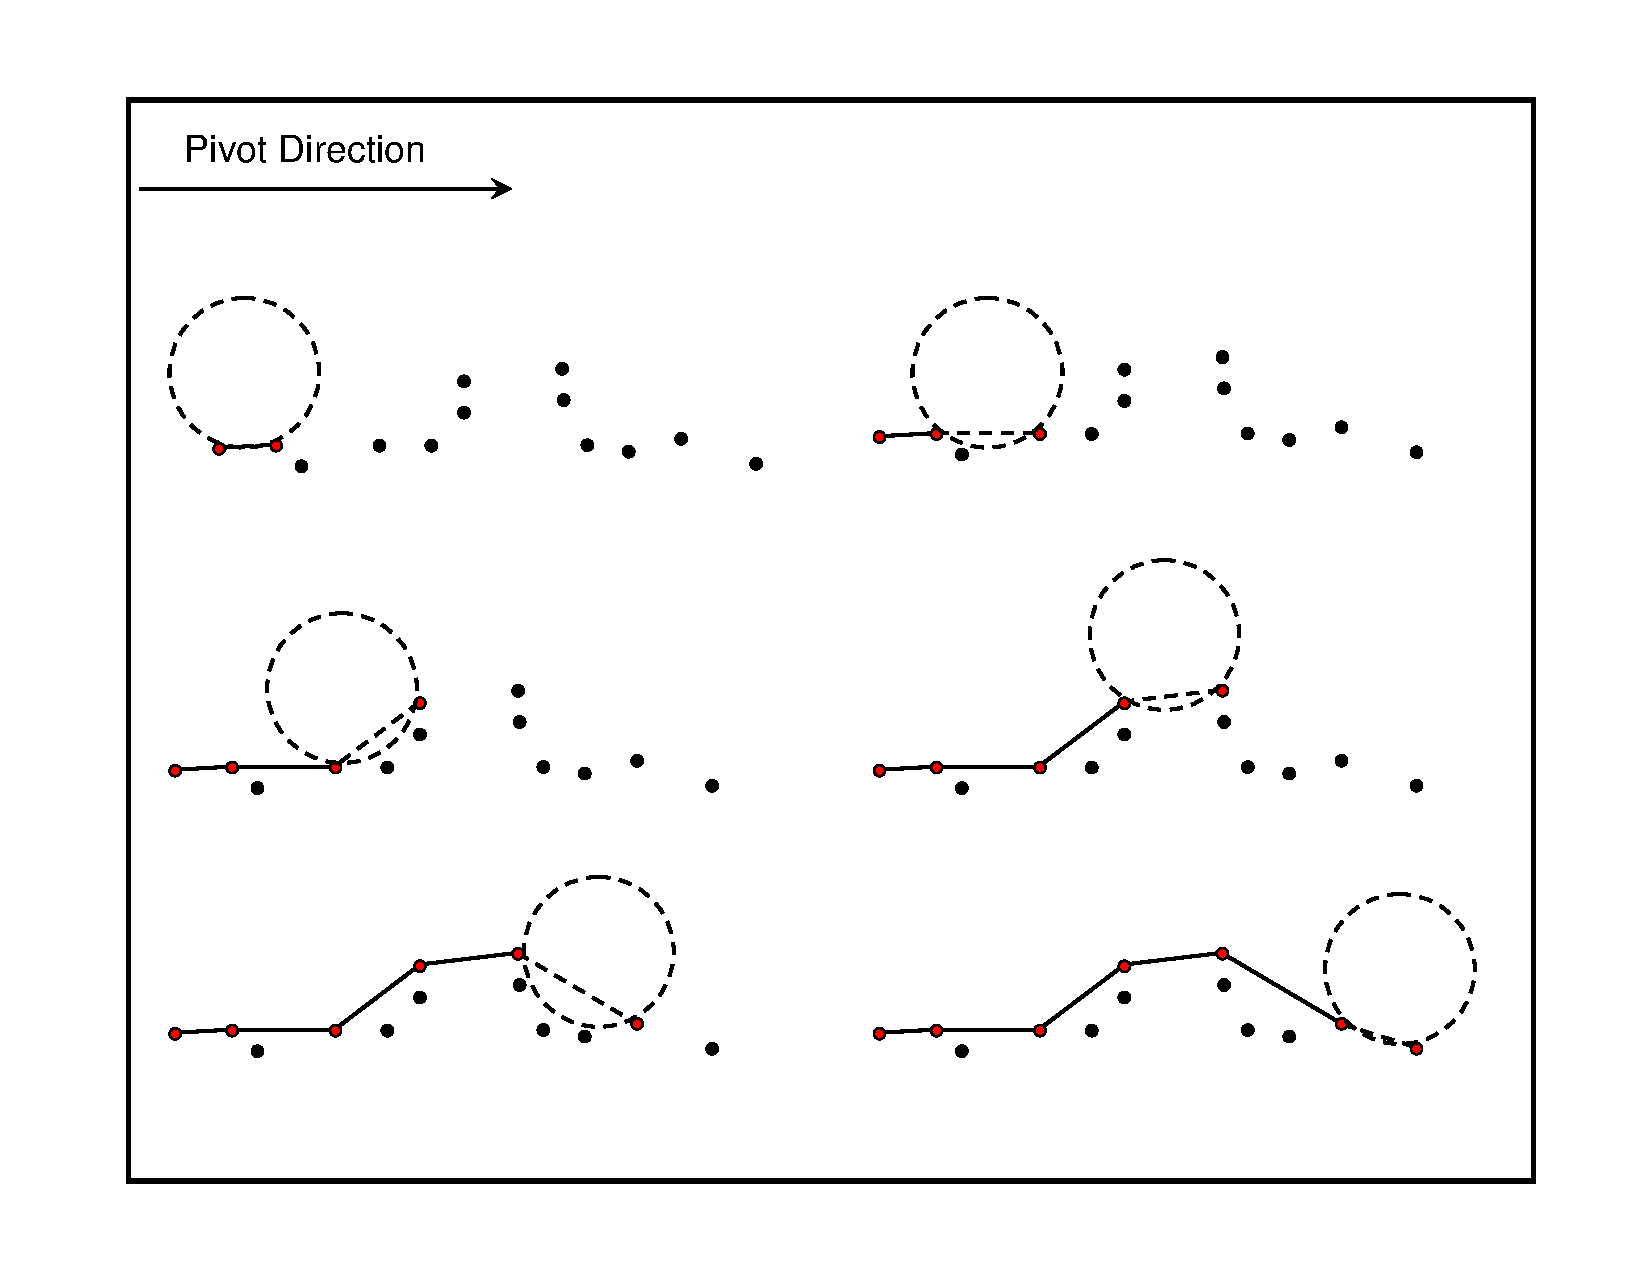
\includegraphics[width=0.8\textwidth]{BPA_init.pdf} \\
(a) \\
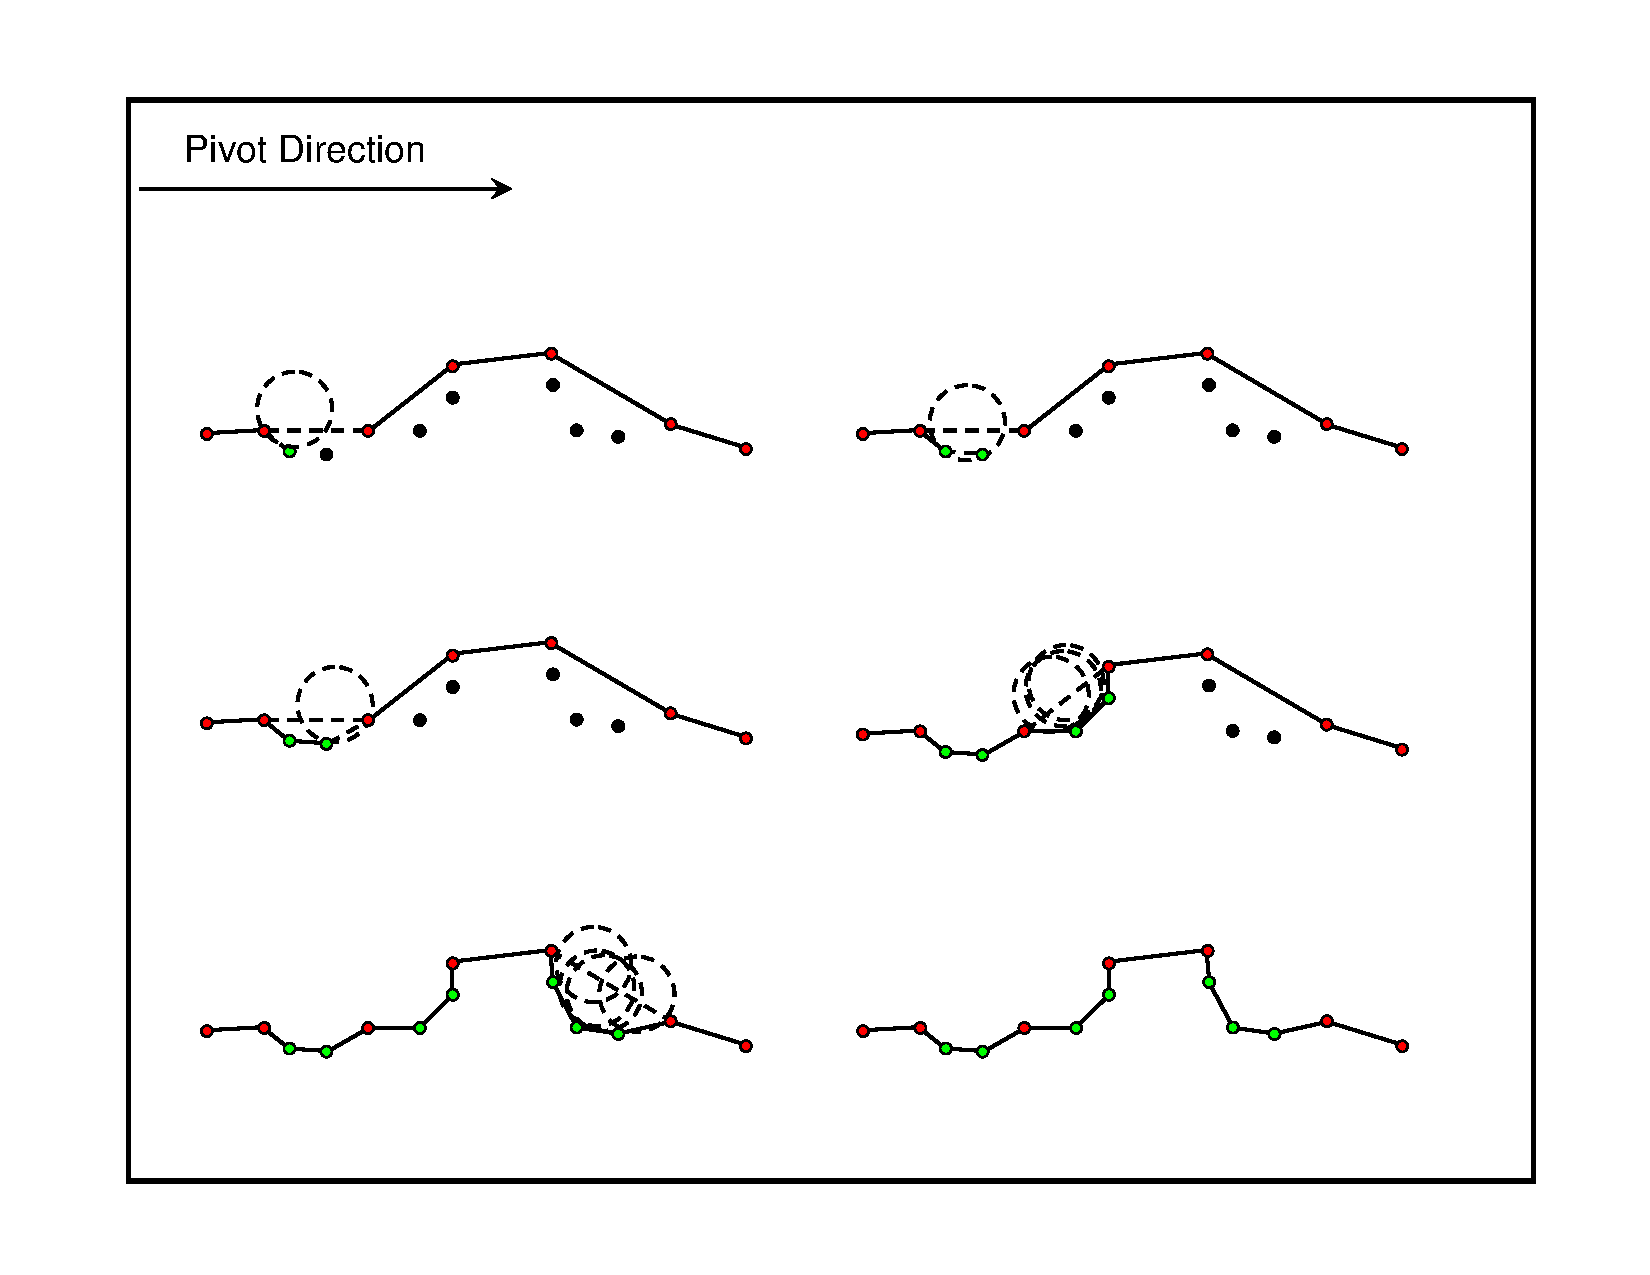
\includegraphics[width=0.8\textwidth]{BPA_refine.pdf} \\
(b)
\end{tabular}
\end{center}
\caption{Adaptive ball pivoting algorithm:
(a) Initial pivoting with a ball of radius 2$r$;
(b) Refinement with a ball of radius $r$.}
\label{fig:BPA}
\end{figure*}


The idea of the BPA is straight-forward:
pivot a ball on a starting point in the image
until it touches another data point as depicted in \Figa{BPA}.
Add the new touched
data point into an ordered list as the vertices of the contour polygon and
set it as the new pivoting point.
Keep doing this pivoting process until all data points are touched.

\section{Boundary Vectorization}
The basic idea behind the proposed framework for contour computation is as follows:
apply BPA on a selected starting point until
either the ball pivots back to the starting point 
which indicates a closed boundary is detected,
or the ball reaches a gap which means this contour is a non-closed
contour and one of the end points is reached.
Because the ball can start pivoting along either clock-wise direction 
or counter clock-wise direction,
another pivoting process at start pivoting from the other direction is conducted.
When both directions have been explored, a contour computation is done.
After this, the refinement process is carried out 
for each line segments using the same BPA algorithm.
For this refinement, the starting point is now the first end point of a line
and the stopping case is that the ball reaches the other point or it reaches a gap.

Here is more detailed description for the algorithm.
At the initial BPA stage, a relatively large radius $r$ is chosen 
as a coarse step to cover all gaps between data points.
The output of the initial BPA, $\boldsymbol{\Phi}$, 
contains an ordered list of the boundary data points $\boldsymbol{P}$ 
and their corresponding directions $\overrightarrow{\boldsymbol{R}}$ 
in which the ball $C$ starts pivoting.
The BPA refinement process applies a smaller radius, say $r' = r/2$,
to $\boldsymbol{\Phi}$ to get more accurate results, as shown in \Figb{BPA}.
For this stage, the length of each line segment formed by adjacent points is checked,
$\ell = \overline{P_0P_1}$, in $\boldsymbol{\Phi}$.
For long line segments, the BPA is applied between the two adjacent points.
When the ball reaches the second end point, a new list of ordered boundary points,
$\boldsymbol{\Phi'}$, is inserted into $\boldsymbol{\Phi}$ between $P_0$ and $P_1$.
This process continues until it finishes 
checking every adjacent point in $\boldsymbol{\Phi}$.
The refinement stops when $r'$ falls below threshold $\tau_r$.

The key parameter for the BPA algorithm to work successfully is finding
a good initial size of the ball for pivoting.
Here are some general guidances for choosing the radius. 
If a contour is known to be a closed polygon,
the initial radius should be big, e.g. the width of an image, 
to cover all gaps along the boundary.
Otherwise, if a boundary consists of sub-boundaries, 
one could select a relative small radius to start.

An example on the proposed framework is shown in \Fig{BPA_refinement}.
The initial BPA takes radius $\tau_r$ = 128,
which produced a coarse contour as shown in \Figa{BPA_refinement}.
\Figb{BPA_refinement} - \Figd{BPA_refinement} show that the contour is becoming more
accurate as the radius $\tau_r$ decreases from 32 to 2. Note that the original
image size is 1024x392 pixels as shown in \Figa{failed_case}.

\begin{figure}[htbp]
\begin{center}
\begin{tabular}{cc}
\fbox{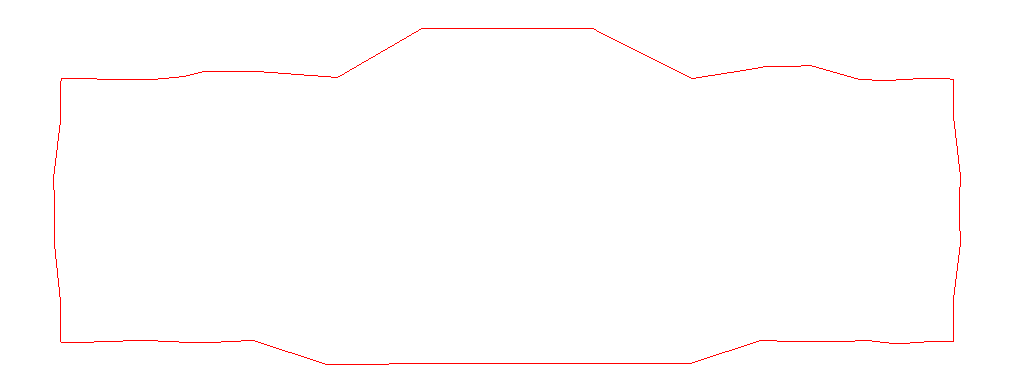
\includegraphics[width=0.45\textwidth]{global_init_refine_with_rad_128.png}} &
\fbox{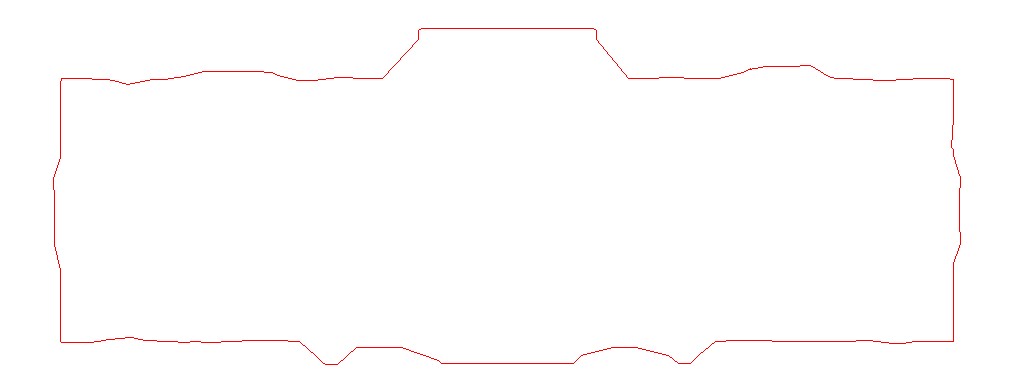
\includegraphics[width=0.45\textwidth]{global_init_refine_with_rad_32.png}} \\
(a) & (b) \\
\fbox{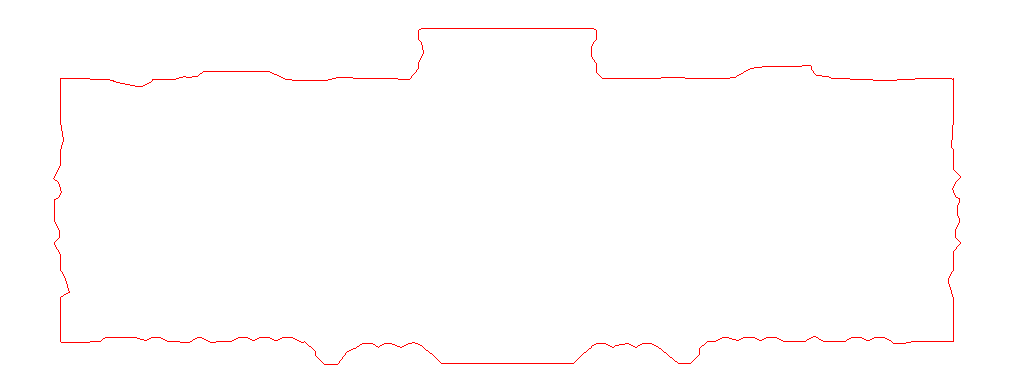
\includegraphics[width=0.45\textwidth]{global_init_refine_with_rad_8.png}} &
\fbox{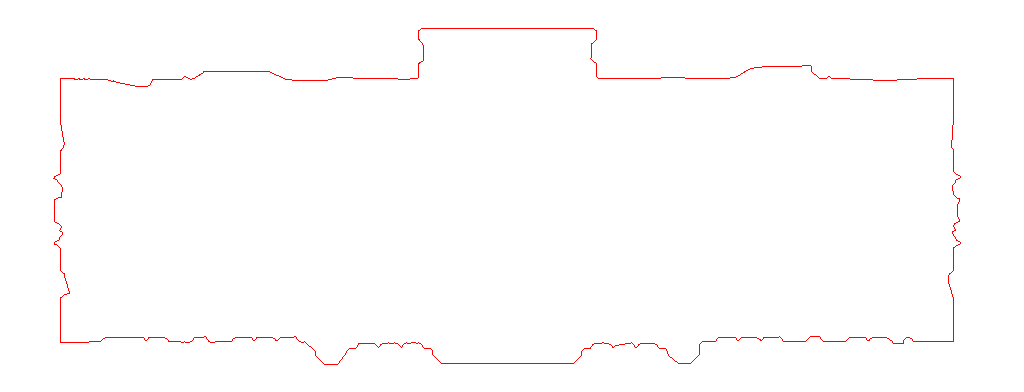
\includegraphics[width=0.45\textwidth]{global_init_refine_with_rad_1.png}} \\
(c) & (d)
\end{tabular}
\end{center}
\caption{Boundary vectorization of a binary image with (a) radius = 128
(b) radius = 32 (c) radius = 8 (d) radius = 2.}
\label{fig:BPA_refinement}
\end{figure}


\begin{figure*}[htbp]
\begin{center}
\begin{tabular}{c}
\fbox{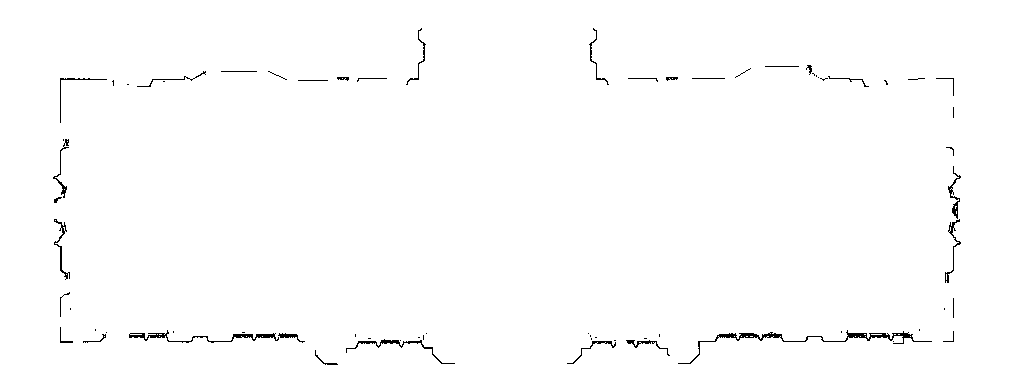
\includegraphics[width=0.7\textwidth]{failed_case.png}} \\
(a) \\
\fbox{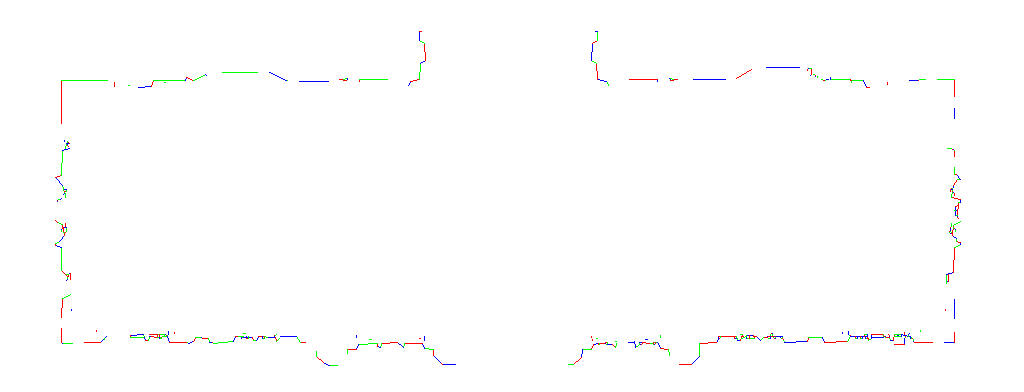
\includegraphics[width=0.7\textwidth]{failed_case_ply.png}} \\
(b) \\
\fbox{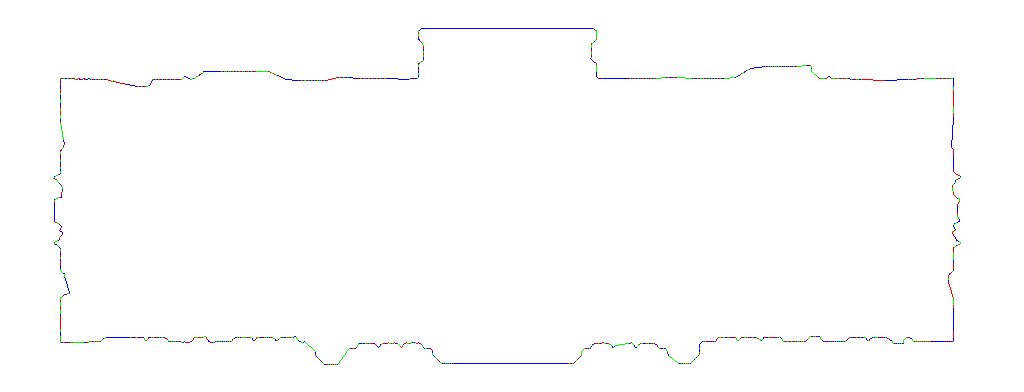
\includegraphics[width=0.7\textwidth]{failed_case_bpa.png}} \\
(c) 
\end{tabular}
\end{center}
\caption{(a) An example of binary image.
(b) The vectorization result based on DP algorithm and
(c) The vectorization result from proposed BPA algorithm.}
\label{fig:failed_case}
\end{figure*}

\begin{figure*}[htbp]
\begin{center}
\begin{tabular}{c}
\fbox{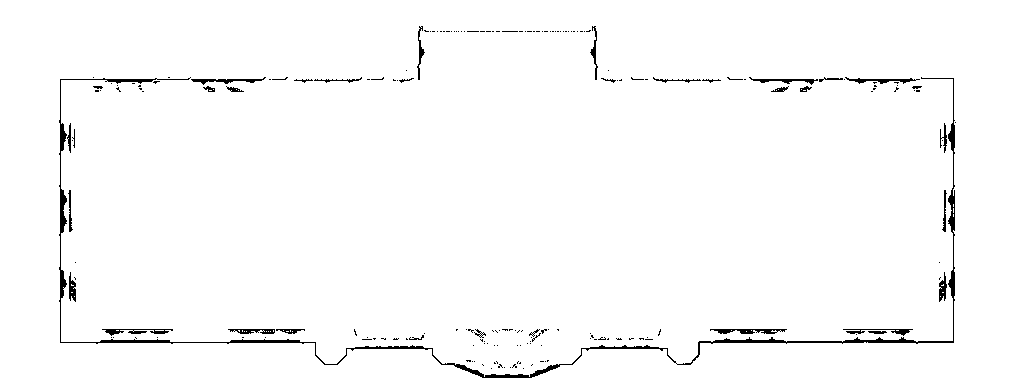
\includegraphics[width=0.7\textwidth]{aaa_image_slice_0529.png}} \\
(a) \\
\fbox{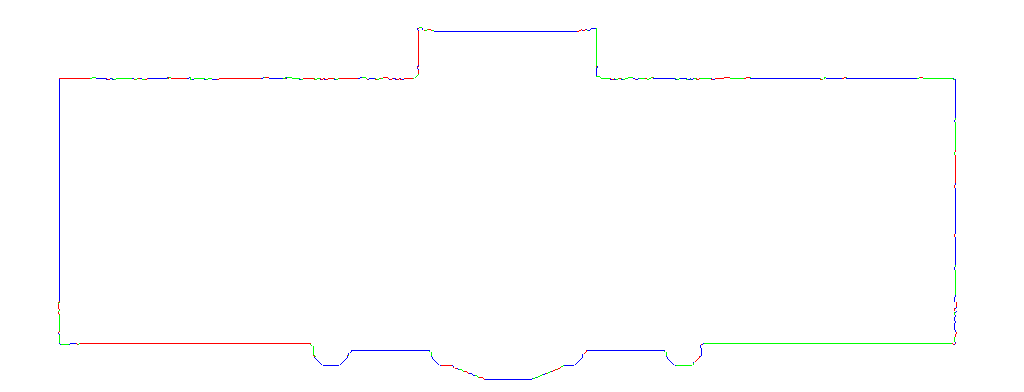
\includegraphics[width=0.7\textwidth]{bbb_image_slice_1024_392_0533_refine_with_rad_1_and_merged.png}} \\
(b) \\
\fbox{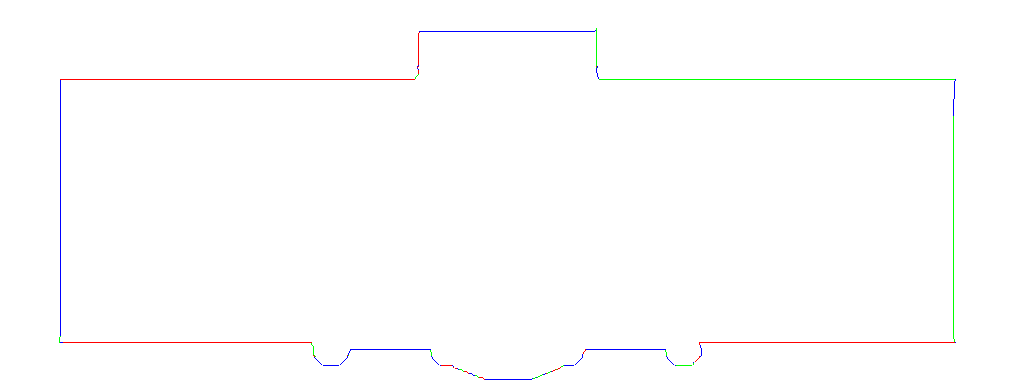
\includegraphics[width=0.7\textwidth]{bbb_image_slice_1024_392_0533_combine_HT_BPA_rad_32.png}} \\
(c)
\end{tabular}
\end{center}
\caption{Boundary vectorization of noisy binary image.
(a) the binary image to be processed.
(b) the contour computed by proposed method.
(c) the contour obtained by simplification with Hough transform.}
\label{fig:HT_BPA_figure}
\end{figure*}

\section{Contour Simplification}
\label{sec:BPA_HT}
%%% Adaptive BPA + HT %%%%

Although the proposed framework is an efficient and straightforward approach to
vectorize the contours of noisy images,
it might produce many short line segments for some special boundaries. 
An example is shown in the upper part of the contour in \Figb{HT_BPA_figure} 
(Please see this in zoomed-in mode). 
Here, each colored segment represents a contour edge.
One way to reduce the number of vertices of the polygon is to apply
the approximation polygon method in \cite{DP_AV}. 
The drawback of this method is that the topological structures, 
such as straight lines, would be lost.
To solve this issue, a Hough transform (HT) based method is proposed to replace
short line segments with long lines and potentially eliminate noisy
or outlier vertices around the boundary.

To combine the adaptive BPA with HT, 
one can first apply the HT algorithm on the original raster image $I$ 
to obtain all straight lines $\boldsymbol{L}$ and sort them by length.
The longer lines give higher confidence to the line structure of the underly images.
Then a dilation operation with 8-connected neighbors on $I$ 
can be used to get the dilation image, $I_d$.
The next step is to measure how well the lines in $\boldsymbol{L}$ match with
data in $I_d$, which determines whether a line in $\boldsymbol{L}$
should be used as a substitution or not.

If a line segment $L$ is found to be a good candidate, the next step is to
find the corresponding part of the BPA points in $\boldsymbol{\Phi}$ for
substitution. The first step is to compute the closest two points
$P_i$ and $P_j$ in $\boldsymbol{\Phi}$ to the two end points of $L$.
If the vertices in $\boldsymbol{\Phi}$ represent a polygon, they will have
a circle layout, i.e., $\boldsymbol{P} = \{ P_0,P_1,\ldots ,P_{n-1}, P_0 \}$.
Assuming $i < j$, there are two possible choices to replace
the series of the points, which are
$\boldsymbol{P_1} = \{ P_i,P_{i+1},\ldots,P_{j-1}, P_j \}$, and
$\boldsymbol{P_2} = \{ P_j,P_{j+1},\ldots,P_{i-1}, P_i \}$.
To determine which one is correct, one can compare the distance, $D$,
from the line $L$ to both set of the points $\boldsymbol{P_1}$ and
$\boldsymbol{P_2}$.
The point set with smaller $D$ is about to be substituted by the line $L$.
\begin{equation*}
D = \underset{\boldsymbol{P_1},\boldsymbol{P_2}}{\operatorname{arg\,min}}\sum{\lVert P_i - L \rVert}
\qquad P_i \in \boldsymbol{P_1} \ \text{or} \ P_i \in \boldsymbol{P_2}
\end{equation*}
where $\lVert P_i - L \rVert$ is the Euclidean distance from point $P_i$ to
line $L$.

After the integration of BPA contour with the Hough transform lines,
the beautified contour is shown in \Figc{HT_BPA_figure}.
Notice that the top part of the contour, which consisted of short line segments, 
was replaced with two long line segments.
As one can see, this process reduces the noise, simplifies the contour, 
and produces clean results for contours with straight line structures.

\begin{figure}[htbp]
\begin{center}
\begin{tabular}{ccc}
\fbox{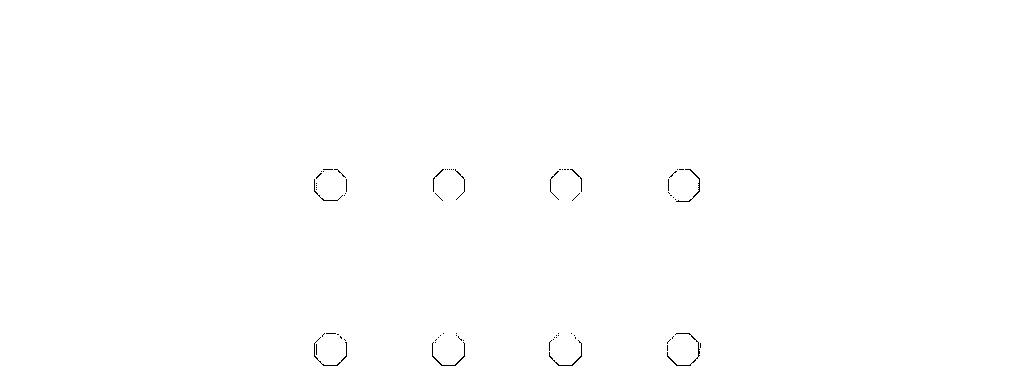
\includegraphics[width=0.3\textwidth]{image_slice_0954.png}} &
\fbox{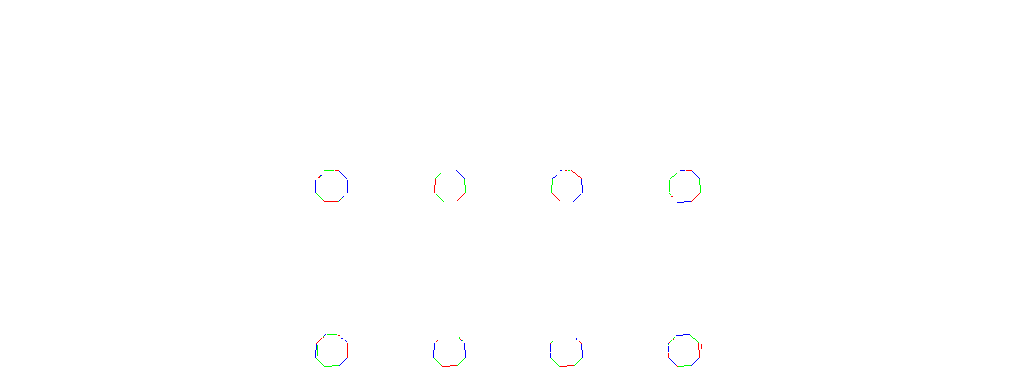
\includegraphics[width=0.3\textwidth]{image_slice_0954_ply.png}} &
\fbox{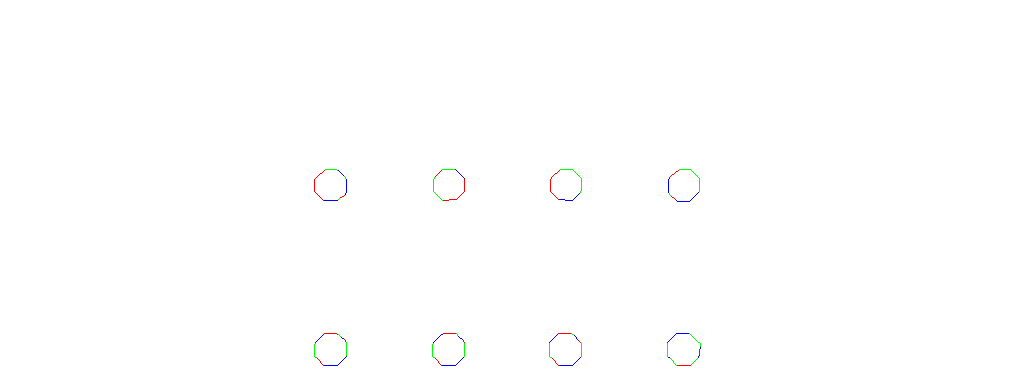
\includegraphics[width=0.3\textwidth]{image_slice_0954_rad_4_and_merged.png}} \\
(a) & (b) & (c) \\
\fbox{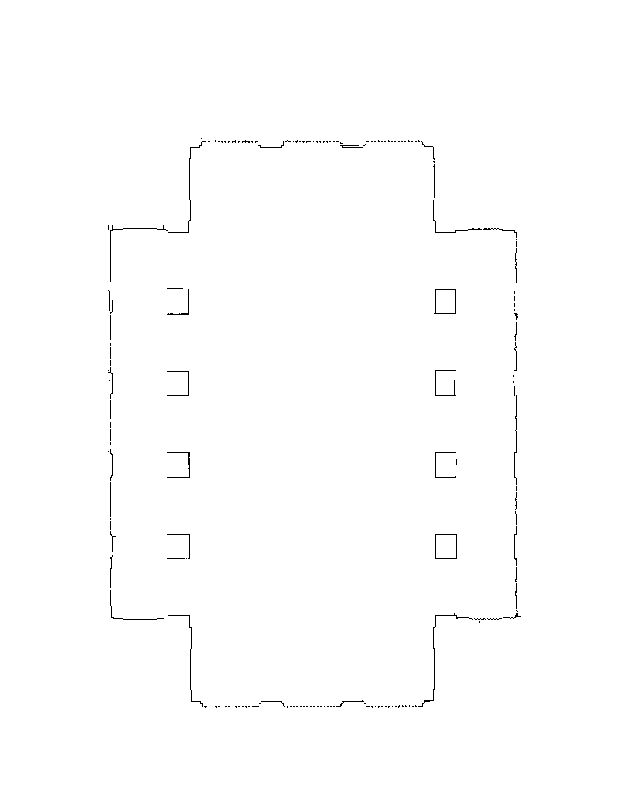
\includegraphics[width=0.3\textwidth]{image_slice_0491_p1.png}} &
\fbox{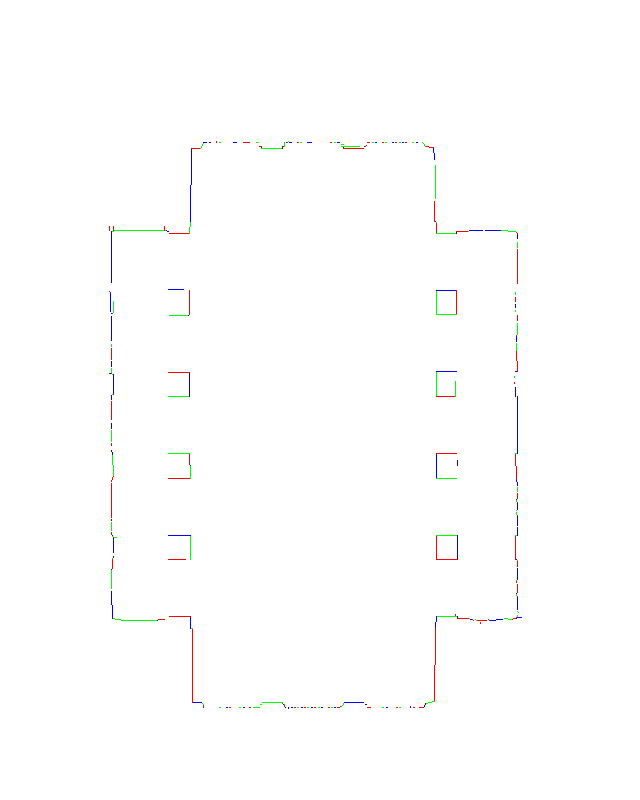
\includegraphics[width=0.3\textwidth]{image_slice_0491_p1_ply.png}} &
\fbox{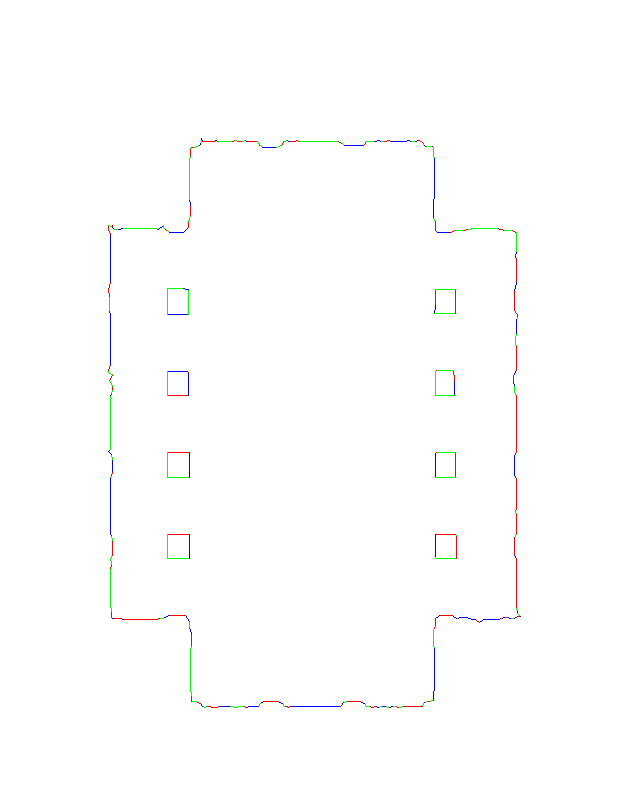
\includegraphics[width=0.3\textwidth]{image_slice_0491_p1_rad_4_and_merged.png}} \\
(d) & (e) & (f) \\
\fbox{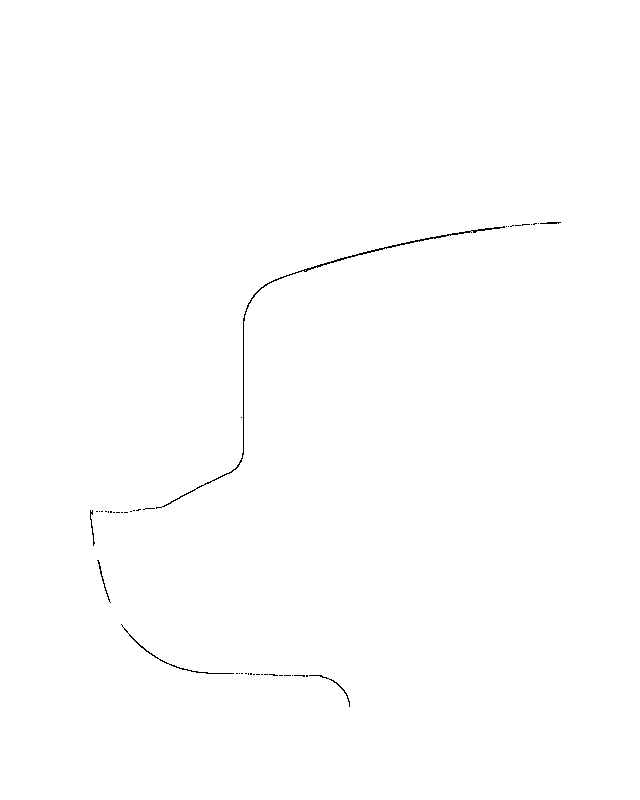
\includegraphics[width=0.3\textwidth]{image_slice_0341.png}} &
\fbox{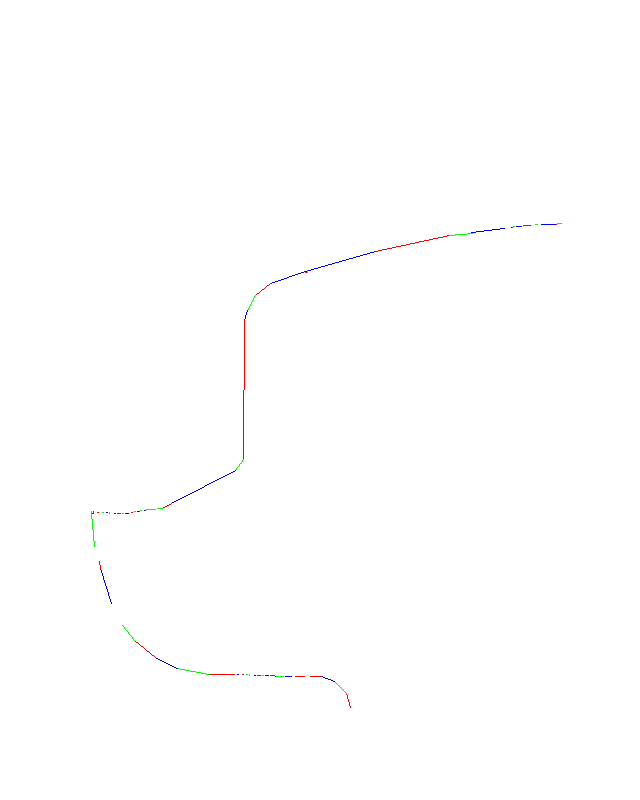
\includegraphics[width=0.3\textwidth]{image_slice_0341_ply.png}} &
\fbox{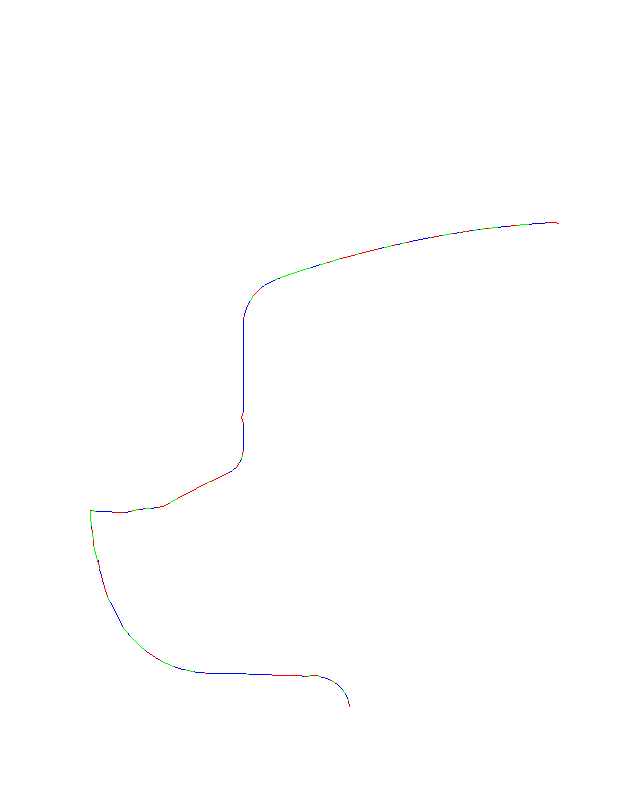
\includegraphics[width=0.3\textwidth]{image_slice_0341_rad_4_and_merged.png}} \\
(g) & (h) & (i) \\
\end{tabular}
\end{center}
\caption{
More experimental results: (a), (d) and (g) show the original noisy binary images.
(b), (e) and (h) show the vectorization results from DP algorithm.
(c), (f) and (i) show the vectorization results from proposed algorithm.}
\label{fig:results}
\end{figure}

In addition to the results shown in \Fig{failed_case} and \Fig{HT_BPA_figure}, more
experimental results are shown in \Fig{results}. In the first row of \Fig{results},
the input image is of size 1024x392 and contains multiple contours.
In the second row, the input image is 800x640 and contains nested contours.
In the third row, the input image is 800x640 and contains a curved contour.
As one can see, the proposed framework can handle all the cases properly 
and fill the holes as expected, which outperformed the standard DP algorithm.


\begin{figure}[htbp]
\begin{center}
\begin{tabular}{c}
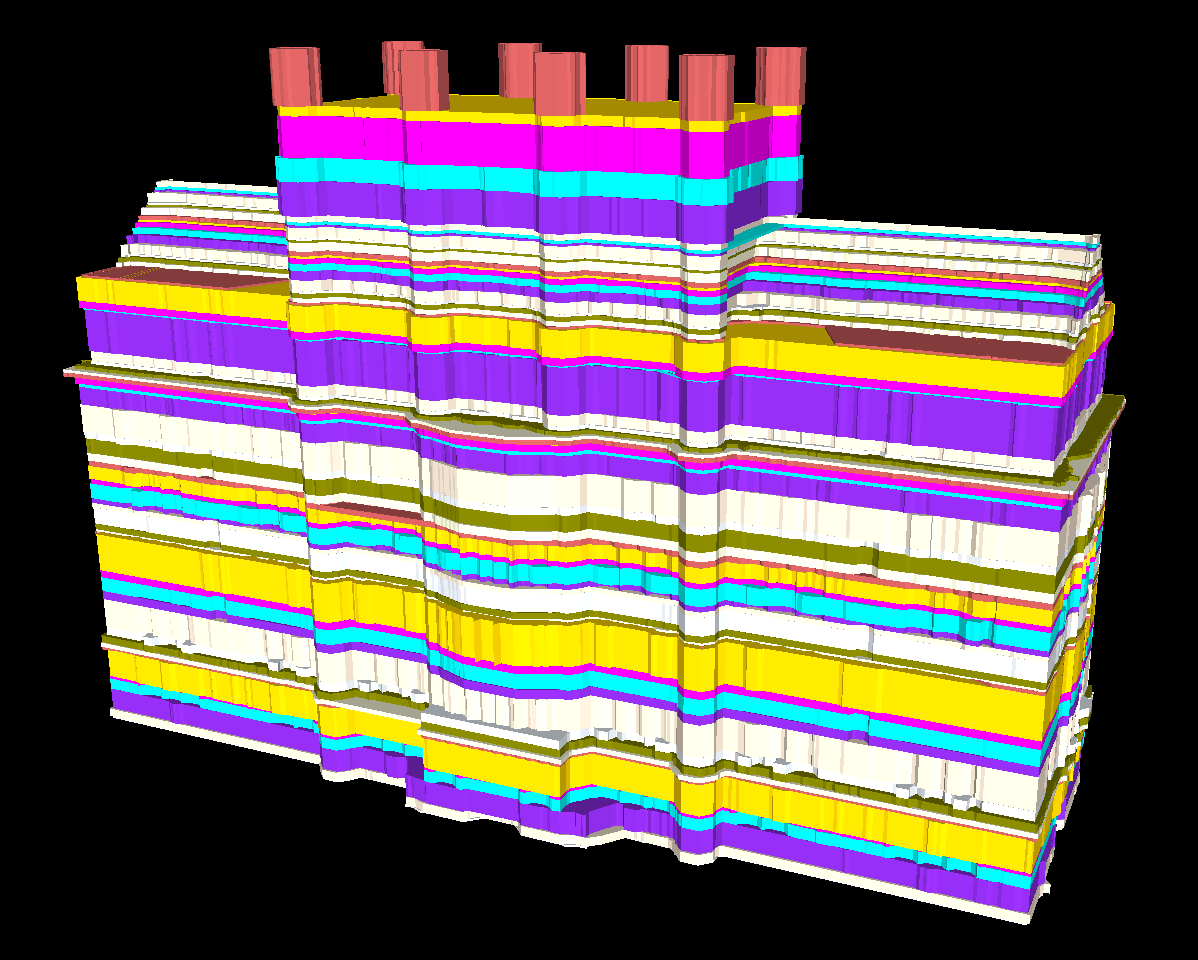
\includegraphics[width=0.8\textwidth]{notaper_8_4.png}
\end{tabular}
\end{center}
\caption{ The reconstructed model based on extrusion operation on keyslices. }
\label{fig:DXF_notaper_model}
\end{figure}

\newchapt{Tapered Structure Detection}{chapt6}{Tapered Structure Detection}

After the keyslices are detected and vectorized, the contours of
$N_K = \{I_{i}, i = 0, ..., K \}$ keyslices are used to represent
the building based on the extrusion operation.
That is, the space between each pair of keyslices, say $I_{i}$ and $I_{j}$,
can be interpolated by the lower keyslice, e.g., $I_{i}$ in this case.
This is valid due to the similarity between the intermediate slices
and the keyslice $I_{i}$.
By modeling a building using this series of keyslices $N_K$, we
significantly reduce the polygon count for urban buildings. 
An example of the reconstructed model is shown in \Fig{DXF_notaper_model}.
This helps make possible 3D web-based applications such as 3D city navigation.

In addition to the extrusion operation, we can further improve the model
and reduce the model size by observing that part of the keyslice images
belong to the same tapered structure, as demonstrated in \Fig{DXF_top}.
\Figa{DXF_top} shows the roof structure
of the reconstructed model based on a keyslice image extrusion operation with
almost half of the keyslice images dedicated to the structure.
After inferring the tapered structure, \Figb{DXF_top} shows the improvement
of the modeling, which is much smoother than the previous model.
In addition, the keyslices needed to represent the building, and its
associated storage, are reduced almost in half.

\begin{figure}[htbp]
\begin{center}
\begin{tabular}{c}
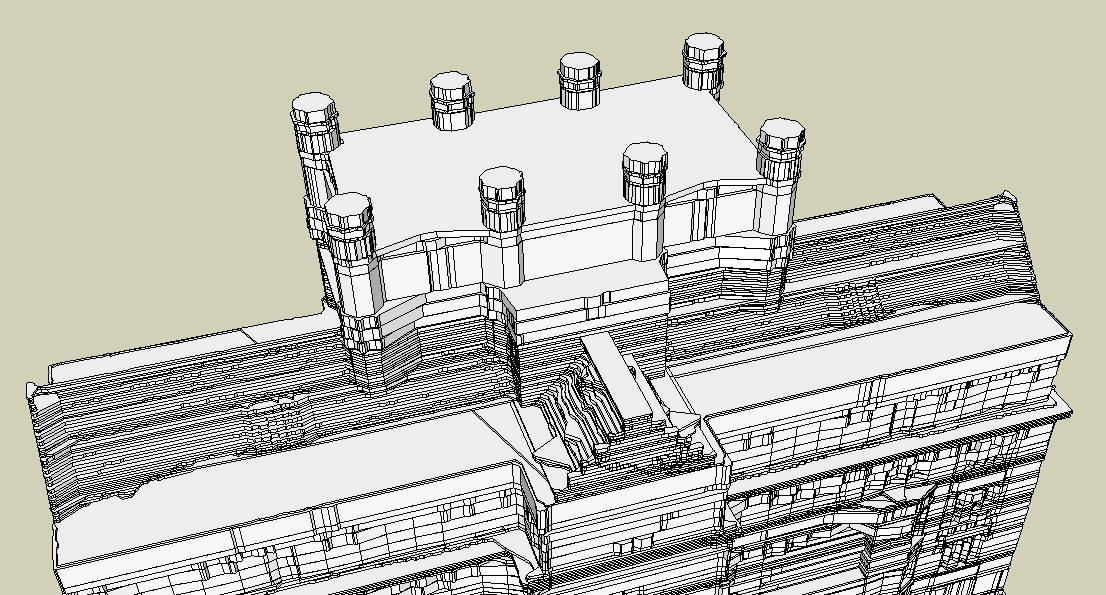
\includegraphics[width=0.7\textwidth]{extrude_1.png} \\
(a) \\
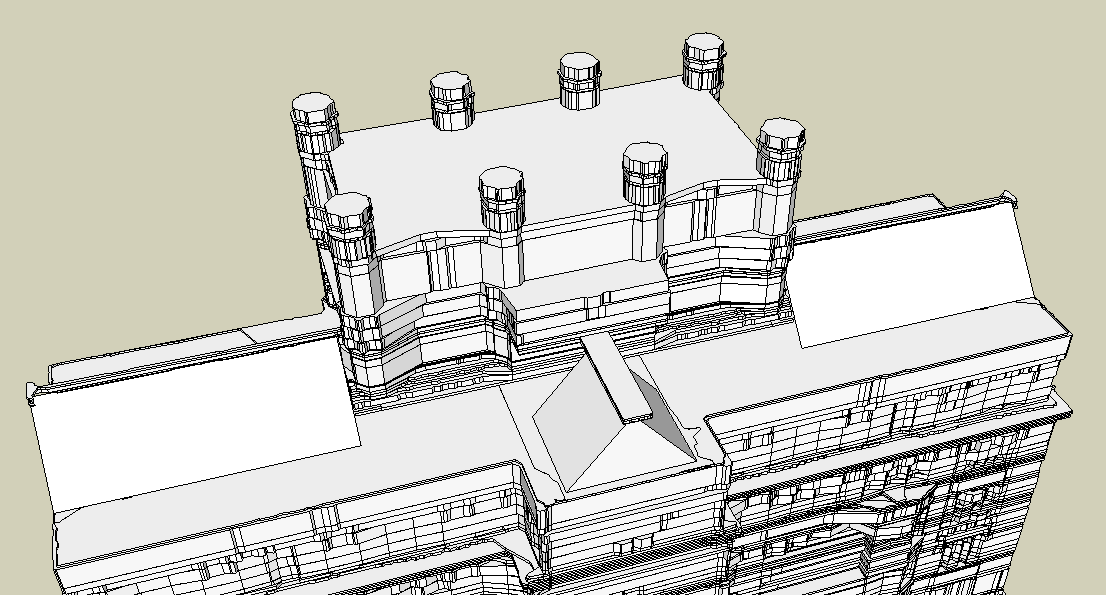
\includegraphics[width=0.7\textwidth]{extrude_2.png} \\
(b)
\end{tabular}
\end{center}
\caption{The top view of the 3D building shown (a) without tapered structures
and (b) with tapered structures.}
\label{fig:DXF_top}
\end{figure}

\section{Inferring Taper Structure}
\label{sec:tsd}

The difficulty in inferring tapered structures is tied to the complexity of
the building structure itself.
Let's assume that the height range for the roof structure is
$H_R = [H_{lo}, H_{hi}]$.
If this is the only existing structure between $H_R$, it is simple and
straight-forward to detect and infer this part.
However, for some complicated structures, such as a mixed layout
of tapered and extruded structures, as depicted in \Fig{taper_seg},
some special treatment is needed to obtain the desired results.
Our approach is based on the divide-and-conquer strategy:
the whole structure $\boldsymbol{U}$ is segmented into independent
sub-structure units, $U_0, U_1, \ldots, U_N$.
Any sub-structure unit $U_i$ is constrained to contain a unique structure,
i.e., either a tapered or an extruded one.
Once each unit $U_i$ is inferred, the whole structure can be modeled by a
union operation of these sub-structures, i.e.,
$\boldsymbol{U} = \bigcup{U_i\{ i = 1,\ldots,N\}}$.
Before segmentation, the potential height ranges $H_R$ containing the tapered
structures must be computed.
This can be done by checking the frequency of the keyslice images.
The structure containing tapered sub-structures will show a wide and uniform
distribution of keyslice images.
This is a very useful clue for $H_R$ detection.

\begin{figure}[htbp]
\begin{center}
\begin{tabular}{c}
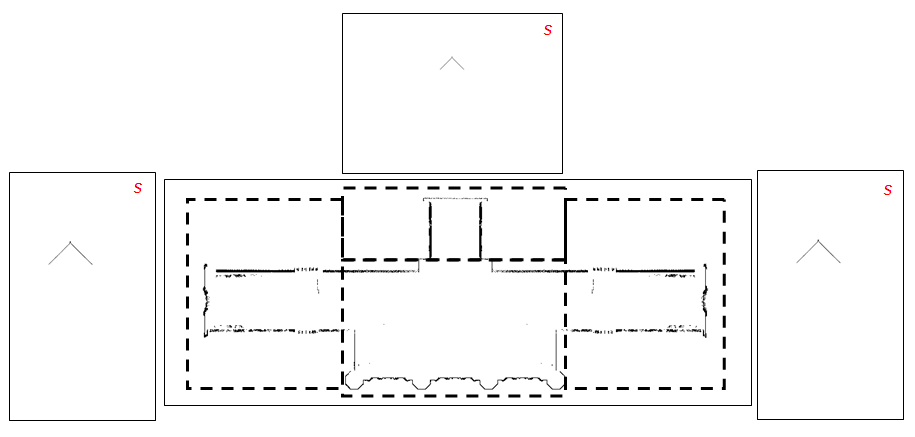
\includegraphics[width=0.8\textwidth]{extrude_3.png} \\
\end{tabular}
\end{center}
\caption{The top 2D slice of the 3D building. }
\label{fig:taper_seg}
\end{figure}

Once the potential height ranges $H_R$ is obtained, the next step is to
segment the whole structure $\boldsymbol{U}$ between $H_R$ into sub-structures,
$U_i, \; i = 0,\ldots,N$.
This is again done by applying the similarity measurement to sliced images
from orthogonal directions.
As before, the 3D data points inside the range of $H_R$ are projected
along both left-right ($X$ axis) and face-inside ($Z$ axis) directions.
Then, the keyslice detection is carried out based on the Hausdorff distance
similarity measurement for both directions.
These keyslices will segment the structure in $H_R$ into subunits of
$U_0, U_1, \ldots, U_N$.

For each subunit $U_i$, we must determine 
whether it represents an extruded or a tapered structure.
This is done by checking in keyslice image $I_k$ of $U_i$ whether there exists
a pattern where two lines intersect with some appropriate angle.
If such a pattern exists in $I_k$, such as the images marked with red $s$ in
\Fig{taper_seg}, the unit $U_i$ is considered to be a tapered sub-structure unit.
Otherwise, $U_i$ is treated as an extruded sub-structure unit.
If $U_i$ is an extruded unit, its contours from the $y-$ axis are vectorized
and is ready for the union operation to obtain $\boldsymbol{U}$.
On the other hand, if $U_i$ is a tapered unit, the bottom and top position
have to be computed so that it can be reconstructed.
To do this, all line segments $\boldsymbol{L}$ in $U_i$ are computed using
the Hough Transform and the intersection point $P_0$ of $\boldsymbol{L}$
indicates the top position of the tapered unit.
The other end points $P_i$ of $\boldsymbol{L}$ are also computed to infer
the bottom shape and position. 
The model enhanced by taper operation is shown in \Fig{DXF_taper_model}.

\begin{figure}[htbp]
\begin{center}
\begin{tabular}{c}
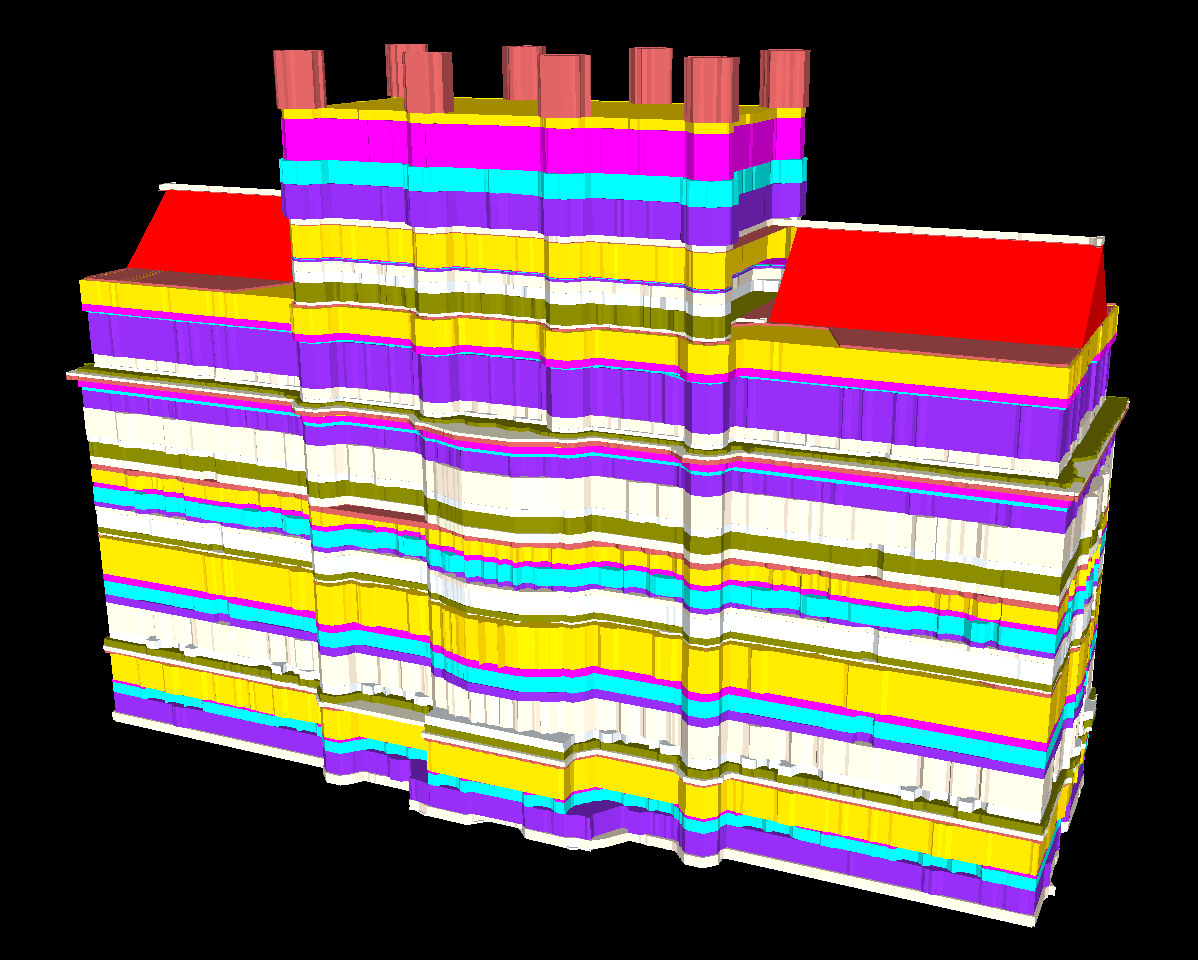
\includegraphics[width=0.8\textwidth]{taper_8_4.png}
\end{tabular}
\end{center}
\caption{ The reconstructed model enhanced by taper operation on roof structure. }
\label{fig:DXF_taper_model}
\end{figure}

\section{Taper-to-point Structure Inference}
\label{sec:tsd_ttp}
The approach we described and illustrated in the previous sections can only be
applied on the inference of taper-to-line structure. 
In addition to this, there is another
type of tapered structure, i.e. taper-to-point structure which appears frequently in 
Gothic architecture, such as churches.
Unlike the taper-to-line, this type of taper structures are not able to be inferred 
through the extruded structure from the orthogonal directions.
However, a nice characteristic of this type of taper structure is that
the vertices of the base geometry converge to a point, which is good clue for inference.
\Fig{DXF_taper_both} shows a synthetic data model consists of both taper-to-point (left)
and taper-to-line (right) structures. 

\begin{figure}[htbp]
\begin{center}
\begin{tabular}{c}
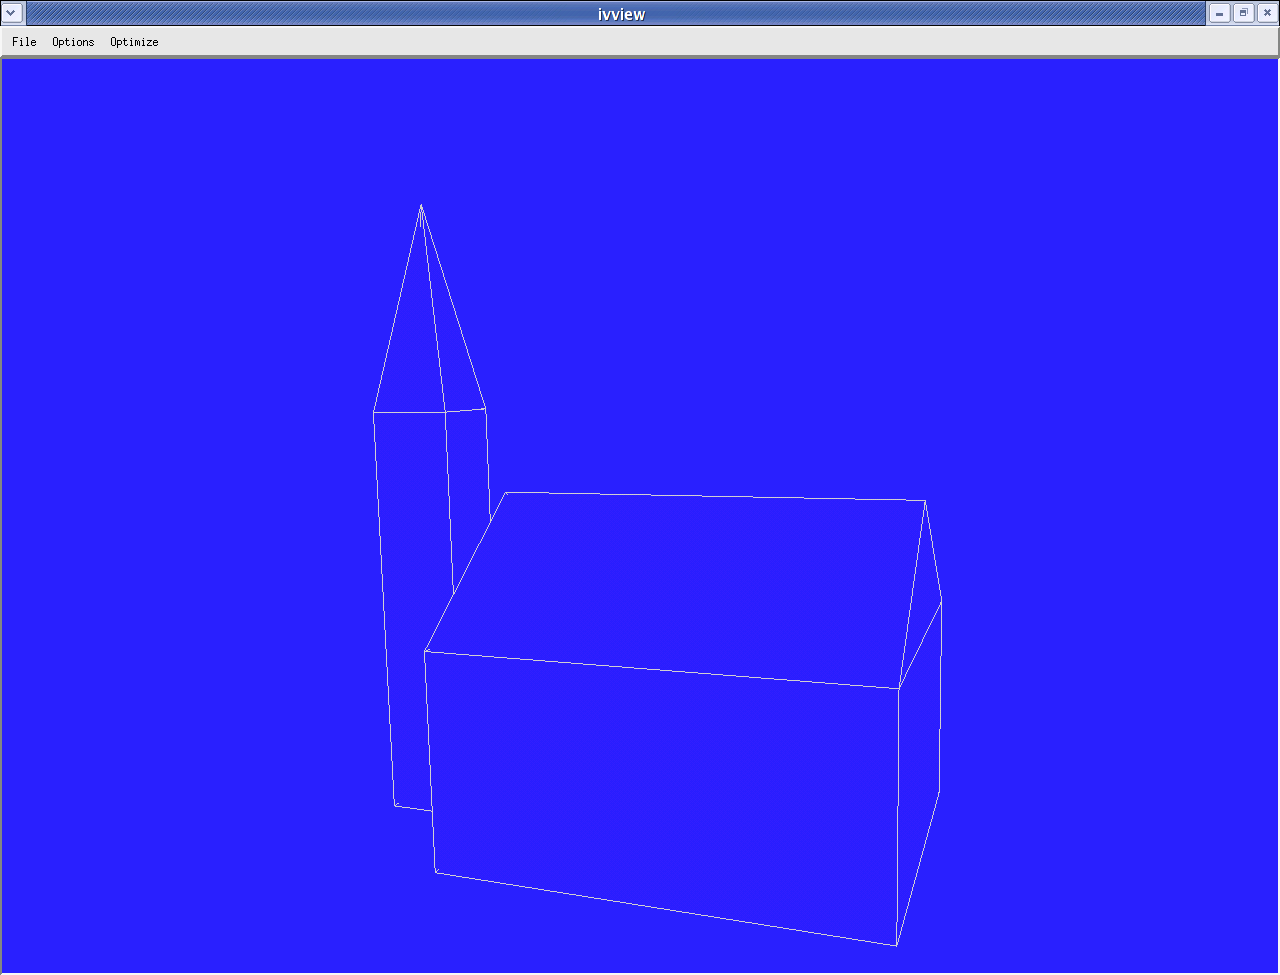
\includegraphics[width=0.8\textwidth]{taper_both_syn.png}
\end{tabular}
\end{center}
\caption{ The synthetic model consists of taper-to-point and taper-to-line structures. }
\label{fig:DXF_taper_both}
\end{figure}

Without loss of generality, we assume that the sliced images of this special structure
can be vectorized by a closed polygon.
Let $S_i$, $S_j$ be two consecutive sliced images and $S_i$
has a smaller boundary than $S_j$. Based on this special structure, $S_i$ will be growing up
to cover $S_j$ by iterative dilation operations. By doing this, we can quickly locate the
bottom and top (a small region representing a point) slices of this special geometry
structure and therefore reconstruct this sub-model using these two slices.
The difference between this structure and the structure of tapering to a line is whether
$S_i$ and $S_j$ have any overlapping or common parts, which is easy to check.




\newchapt{Algorithm Analysis}{chapt7}{Algorithm Analysis}

%%%%%%%%%%%%%%%%%%%%%%%%%%%%%%%%
%%%%%%  Algorithm Analsysis  %%%
%%%%%%%%%%%%%%%%%%%%%%%%%%%%%%%%
\section{Algorithm Analysis}
\label{sec:PE_AA}

\begin{algorithm}
\caption{The Adaptive Hough Transform Algorithm}
\label{alg.AHT}
\begin{algorithmic}[1]
\Procedure {AHTA}{$I$, $\boldsymbol{L}$}
\While {$true$}
\State $\bigcup{(\rho, \theta)} \leftarrow HT (I)$  \Comment{regular hough transform to get a set of lines}
\State $n \leftarrow 0 $
\For {each $(\rho, \theta) \in \bigcup{(\rho, \theta)} $}
     \State $c \leftarrow num(I, \rho, \theta)$  \Comment{compute \# of points falling onto line ($\rho, \theta$)}
     \If {$n < c$}
         \State $n \leftarrow c$
         \State $\rho_{max} \leftarrow \rho$
         \State $\theta_{max} \leftarrow \theta$
     \EndIf
\EndFor
\If {$n > \epsilon $}   \Comment{ sanity check for the line ($\rho_{max}, \theta_{max}$) }
\State $\boldsymbol{L} \leftarrow (\rho_{max}, \theta_{max})$
\State $update(I, \rho_{max}, \theta_{max})$ \Comment{ remove points falling onto line ($\rho_{max}, \theta_{max}$)}
\Else
\State $break$
\EndIf
\If {$\omega(I) < \epsilon$} \Comment{ check how many points left }
\State $break$
\EndIf
\EndWhile
\EndProcedure
\end{algorithmic}
\end{algorithm}

The Adaptive Hough Transform (AHT) algorithm stems from the original Hough transform algorithm.
The function $HT()$ is just a regular Hough Transform (HT), which is $O(L)$ for line detection. 
Here $L$ is the data point in 2D image.  The computation of the number of points covered by 
each line  ($\rho, \theta$) detected by $HT$ is of $O(L)$ complexity.
The sanity check and image update function $update()$ is most of query and comparison operation, which is
$O(1)$ complexity. Because we are dealing with bounded number of data points, and the data points
on the longest line of each iteration are removed for each iteration, the AHT will quickly converge.
Because the 3D point cloud data has been projected to 2D image, the worst case for 3D data points is
$O(N)$, where $N$ is the total number of 3D points.

The space complexity of AHT algorithm is bounded by the space complexity of the $HT()$ algorithm. 
Because we are only working on line detection of 2D images, the space complexity is $O(N_\rho * N_\theta)$, 
where $N_\rho$ and $N_\theta$ represents the number of bins for quantizing the value of $\rho$
and $\theta$ respectively. For example, for a image of size 300x400, if we quantize the length $\rho$
with one bin for each pixel, the $N_\rho$ would be 500. Also, if we quantize the the angle with one
bin for a degree, the $N_\theta$ would be 180. Based on this, the space complexity for this example 
can be easily obtained. The precise of the Hough transform algorithm is depend on the quantization 
of the parameters $\rho$ and $\theta$. The more bins are used for quantization, the more precise the
results will be, which implies more space are needed for the algorithm.


\begin{algorithm}
\caption{The 2D Adaptive Ball-Pivot Algorithm}
\label{alg.ABPA}
\begin{algorithmic}[1]
\Procedure {ABPA}{$I$, $\boldsymbol{L}$}
\State $L \leftarrow \emptyset$
\State $P, P_0 \leftarrow S(I) $ \Comment{compute the $seed$ point assigned to $P$ and $P_0$}
\State $r \leftarrow W$ \Comment{initialize radius $r$ with a large value $W$}
\While {$true$}  \Comment{initial BPA stage}
   \State $append(L, P)$ 
   \State $P_i \leftarrow BPA(P, I, r)$ \Comment{regular 2D BPA}
   \If { $P_i = P_0 $ } 
      \State $break$ \Comment { complete the initial BPA }
   \EndIf
   \State $P \leftarrow P_i$ \Comment { find a new vertex $P$ for the contour $L$}
\EndWhile

\State $r \leftarrow W'$ \Comment{a smaller radius $W'$ for refinement}
\While {$r > \epsilon$} \Comment {iterative BPA refinement}
   \For { each line $\overline{P_iP_j} \in \boldsymbol{L} $}
      \State $L' \leftarrow \emptyset$
      \State $P \leftarrow P_i$
      \While {$true$}
         \State $append(L', P)$ \Comment{construct a sub contour $L'$}
         \State $P_k \leftarrow BPA(P, I, r)$ 
	 \If { $P_k = P_j $ } \Comment{stop when reaching the other point}
	    \State $substitute(L, P_i, P_j, L')$ \Comment{refine $\overline{P_iP_j}$ with $L'$}
	    \State $break$
	 \ElsIf { $isGap(L', P_k)$ }  \Comment{stop when reaching a gap}
	    \State $break$
	 \EndIf
	 \State $P \leftarrow P_k$ \Comment { find a new vertex $P$ for $L'$}
      \EndWhile
   \EndFor
   \State $r \leftarrow r/2$  \Comment{reduce the radius for next iteration}
\EndWhile
\EndProcedure
\end{algorithmic}
\end{algorithm}

The 2D adaptive ball-pivot algorithm (ABPA) is summarized in Algorithm \ref{alg.ABPA}. 
The seed computation $S()$ is to randomly pick up a good starting point, which
is only $O(1)$ complexity. The $append()$ function is to concatenate the control 
points, which is only $O(1)$ complexity. The regular 2D ball-pivot algorithm, $BPA()$,
carries out the geometry computation on each control point based on the size of the
radius of the ball or circle. Basically, for each pivoting of the ball, the area 
in the image covered by this pivoting is checked. If there is a data point contained
by this area, the pivoting ends for this control point. 
The complexity for computing the whole potential pivoting area is $O(n)$???, the
complexity to pick up the minimum angle of the pivoting is $O(1)$, therefore, the 
complexity for the whole 2D $BPA()$ is $O(n)$. 

For the refinement process, each line $\overline{P_iP_j}$ of the boundary generated
in the previous iteration is checked using the same algorithm in $BPA()$. This only
takes $O(n)$ complexity. The $substitute()$ and $isGap()$ function is just to insert
a extra point or a simple algebra computation, the complexity for both operations is 
$O(1)$, Because the round of the refinement process is bounded by a predefined constant 
number, say $c$, the complexity of this refinement is also bounded by $O(c*n) = O(n)$. 

The implementation of the ABPA uses O(m) memory space, where m is the size of the 2D image.
This complexity includes the enqueue/dequeue the control points of the boundary, the 
pivoting geometry computation and the $substitute()$ and $isGap()$ computations. Since
the user can control the size of slices, memory requirements can be tailored to the
available hardware. 

\begin{algorithm}
\caption{The Keyslice Detection Algorithm}
\label{alg.KSD}
\begin{algorithmic}[1]
\Procedure {Hausdorff}{$I$, $N$}
  \State $K \leftarrow \emptyset$  \Comment{vector to store the indexes of keyslices}
  \State $I_r \leftarrow I_0$
  \For { $i \leftarrow 1, N-1 $}
    \State $d_1 \leftarrow dis(I_r, I_i) $
    \State $d_2 \leftarrow dis(I_i, I_r) $
    \State $d_{HD} \leftarrow avg(d_1, d_2) $ \Comment {average Hausdorff distance}
    \If { $d_{HD} > \epsilon $}
       \State $I_r \leftarrow I_i$  \Comment{update the reference image}
       \State $ append(K, i) $
    \EndIf
  \EndFor
  \State \textbf{return} $K$
\EndProcedure

\Procedure {Curvature}{$I$, $N$}
  \State $K \leftarrow \emptyset$  \Comment{vector to store the indexes of keyslices}
  \State $V \leftarrow 0$ \Comment {initialize the counter to 0}
  \For { $i \leftarrow 0, N-1 $}
     \State $\bigcup{C} \leftarrow curv(I_i)$ \Comment{curvature computation on image $I_i$}
     \State $\bigcup{c} \leftarrow mapping(\bigcup{C}) $ \Comment{mapping the curvature to indexes}
     \For {each $c \in \bigcup{c}$ }
        \State $V(c) \leftarrow V(c) + 1$ \Comment{increase the number of curvature observed}
     \EndFor
  \EndFor
  \For { each $c \in \bigcup{c}$ }
     \If { $V(c) > \epsilon $}  \Comment {validate the curvatures}
	\State $append(K, c)$
     \EndIf
  \EndFor
  \State \textbf{return} $K$
\EndProcedure

\Procedure {KSDA}{$I$, $S$}
\State $K_1 \leftarrow Hausdorff(I, S)$ \Comment{keyslices computed by Hausdorff distance}
\State $K_2 \leftarrow Curvature(I, S)$ \Comment{keyslices computed by Curvature}
\State $K \leftarrow merge(K_1, K_2)$
\EndProcedure
\end{algorithmic}
\end{algorithm}

The idea of keyslice detection is described in Algorithm \ref{alg.KSD}. 
Essentially, the algorithm consists of two independent procedures. 
The function $Hausdorff()$ is conducting Hausdorff distance based keyslice
detection. A lookup table $t$ is created for the implementation of $Hausdorff()$. 
This lookup table is created by computing for each pixel $p$ in the reference image $I_r$,
how far is $p$ to the nearest data point. If $p$ itself is a data point, the distance is 0.
The complexity of constructing $t$ bounded by $O(w*h)$, where $w$ and $h$ are the image
width and height respectively. Once $t$ is computed, the function $dis()$ is only
$O(1)$ complexity which basically doing queuing from $t$. Therefore, the function $Hausdorff()$
takes $O(n)$ complexity. 
For procedure $Curvature()$, the function $curv()$ which computes curvatures
in the orthogonal direction is of $O(n)$ complexity. The $mapping()$ function and
the remaining steps mainly consists of couple of algebra computation, which takes $O(1)$ complexity. 
Therefore the procedure $Curvature()$ is of $O(n)$. Overall, the algorithm $KSDA()$ takes
$O(n)$ computation complexity for keyslice detection. 

For the space complexity, the keyslice detection algorithm is similar to adaptive ball-pivot
algorithm and uses $O(m)$ memory for computation. Again, the memory usage can be tailored to 
available hardware based on user settings.


\newchapt{Performance Evaluation}{chapt8}{Performance Evaluation}


%%%%%%%%%%%%%%%%%%%%%%%%%%%%%%%%
%%%%%%   Experimental Results%%%
%%%%%%%%%%%%%%%%%%%%%%%%%%%%%%%%
\section{Experimental Results}
\label{sec:IR_OUT}

The results of the extrusion and tapered structures computation,
together with keyslice image vectorization, are stored in the 2D
image coordinate system. To generate the final 3D model, these
data need to be transformed back into the 3D world coordinate system.
Let $P(x,y)$ be a point in the 2D image coordinate system, and let $P'(x,y,z)$
be the 3D world coordinate of $P$, where $y$ is the depth coordinate.
For all points in the same contour, the points lie in the same plane and
hence have the same value of $y$.
The equation for transforming $P$ back to $P'$ is a reverse transformation
of $\boldsymbol{T_0}$ in \Eq{image_slicing}:
\begin{equation}
[\,x^{3D},\; y^{3D},\; z^{3D}\,]^T = [\,\eta\cdot x^{2D} + X_{MIN},\; \zeta + Y_{MIN},\; \eta\cdot z^{2D} + Z_{MIN}\,]^T
\label{eq:ir2dxf}
\end{equation}
where $\eta=1/\omega$ and $\zeta=\kappa\cdot\delta$. Here, $\kappa$ is the
index of the 2D slice and $\delta$ is the height of a slab, as described
in \Sec{image_slicing}.
\Figd{IR_2_DXF} shows an exterior 3D model generated by the above
transformation.

\begin{figure*}[htbp]
\begin{center}
\begin{tabular}{c}
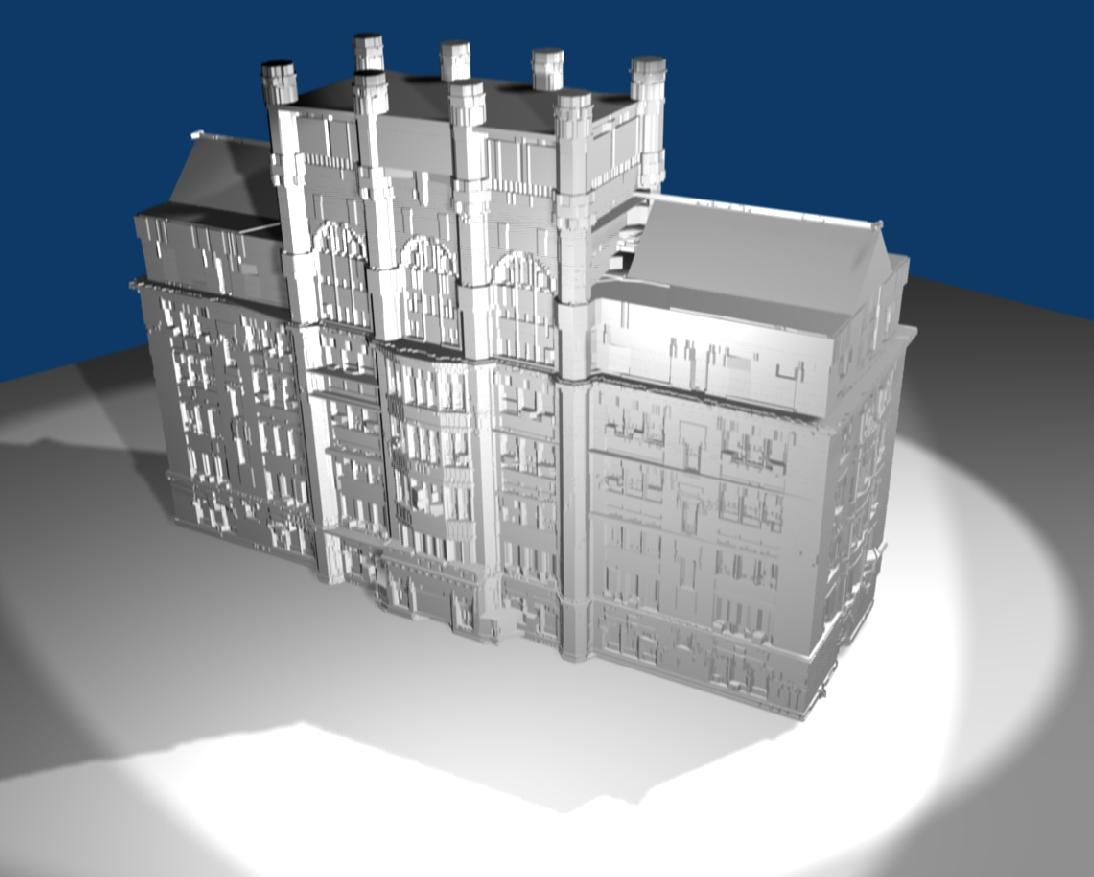
\includegraphics[width=0.8\textwidth]{HunterShaded.jpg} \\
(a) \\
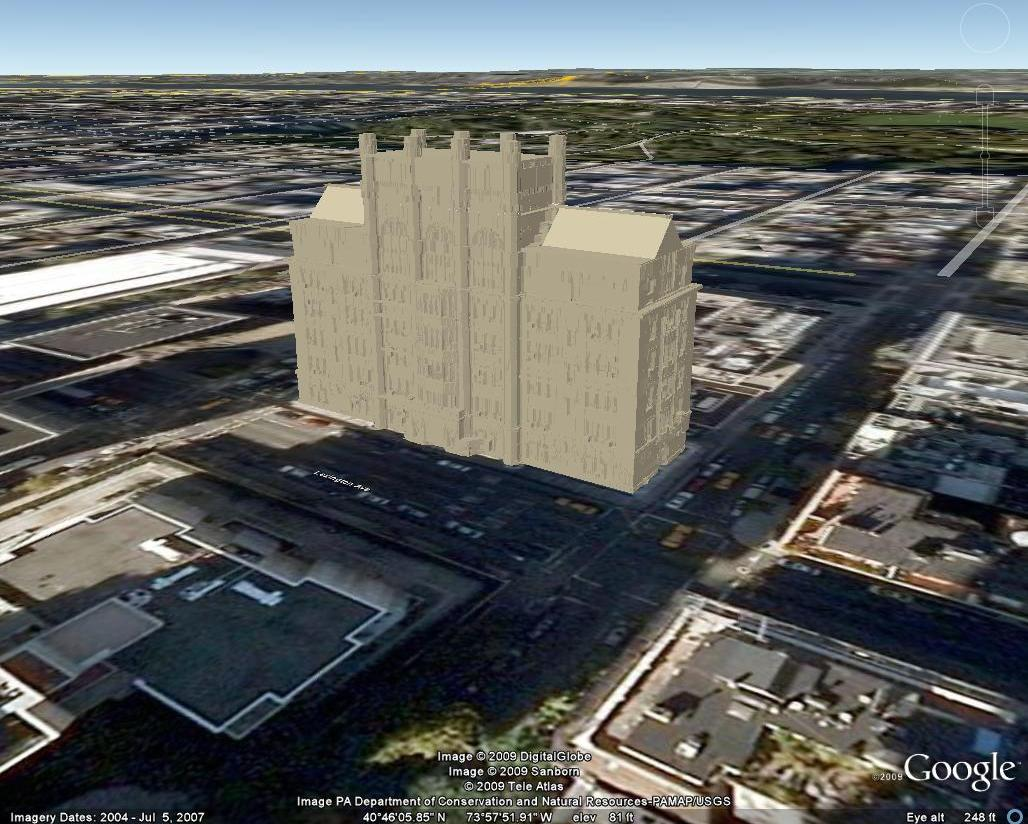
\includegraphics[width=0.8\textwidth]{HunterGE.jpg} \\
(b)
\end{tabular}
\end{center}
\caption{ (a) rendering of lightweight reconstructed model.
(b) The placement of the 3D model on Google Earth.}
\label{fig:OUT}
\end{figure*}

\begin{figure*}[htbp]
\begin{center}
\begin{tabular}{c}
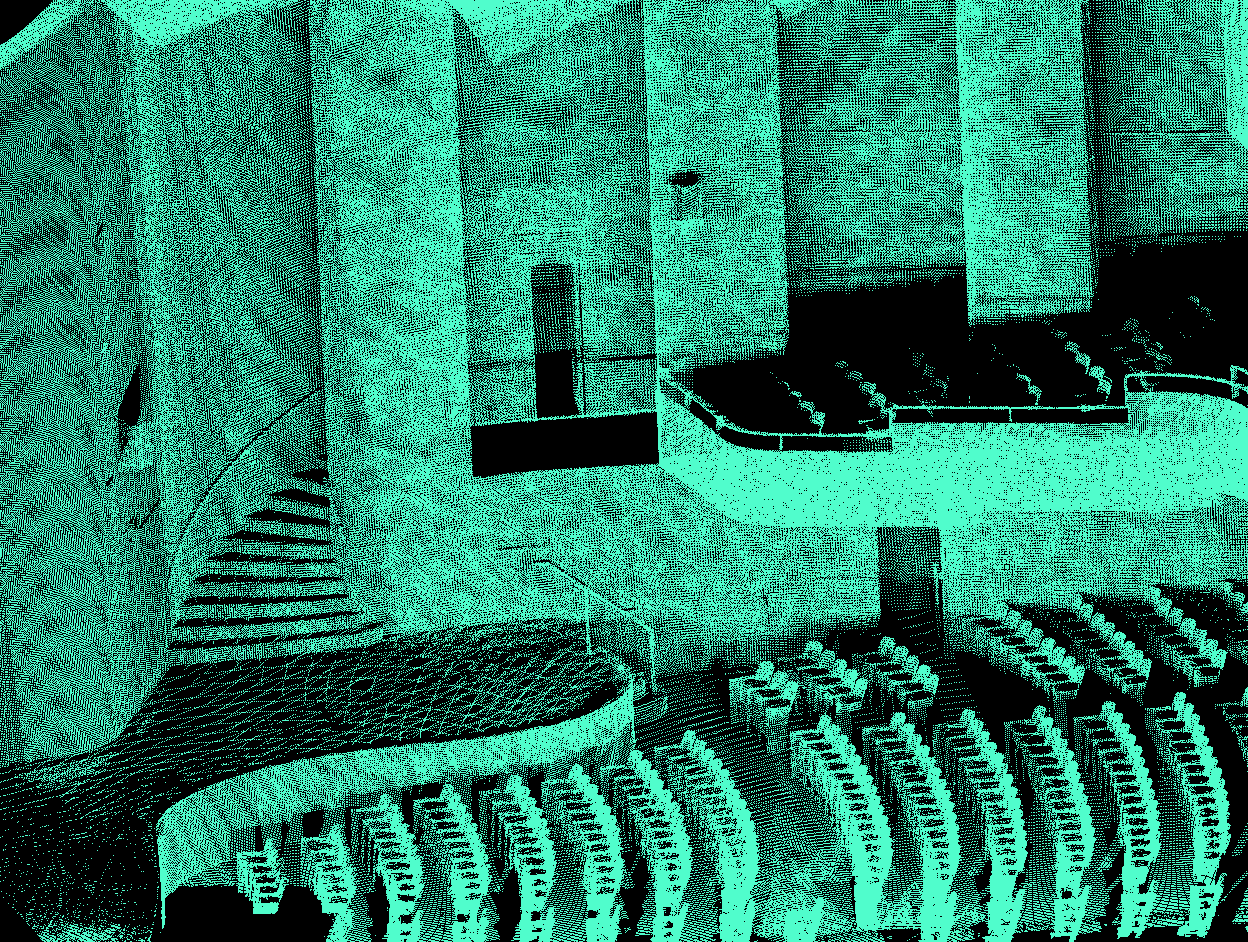
\includegraphics[width=0.8\textwidth]{range_crop.png} \\
(a) \\
\includegraphics[width=0.8\textwidth]{HunterTheatreShaded.jpg} \\
(b)
\end{tabular}
\end{center}
\caption{The model of an interior scan. (a) Point cloud data and the
(b) reconstructed lightweight 3D model.}
\label{fig:IN}
\end{figure*}

In addition to exterior models, we have also applied the lightweight
reconstruction algorithm to the range data of interior scans.
The snapshot of an interior scan is shown in \Figa{IN}
and its reconstructed 3D model is shown in \Figb{IN}.
This model is primarily reconstructed using the extrusion unit
upon the main structures of the interior.
The chairs and some other fine details were manually culled.
Please note that the model generated in \Figb{IN} is of low resolution.
Any lost detail may be recaptured by using a smaller threshold $\tau_d$
to obtain higher resolution models.

To measure the error of a reconstructed 3D model, we first transform it
to the 3D point cloud coordinate system.
The error $E$ is measured as the distance between the 3D points in the cloud
to their closest planes in the reconstructed model $M$:
\begin{equation}
E = \frac{1}{|X|}\sum_{x\in{X}}{d^2(x, M)}
\label{eq:em}
\end{equation}
where $X$ is the set of 3D points in the point cloud, and distance
$d(x, M) = \text{min}_{p \in M}\lVert x - p \lVert$ is the minimum
Euclidean distance from a 3D point $x$ to its closest face $p$ of $M$.

\begin{figure} [htbp]
\begin{center}
\begin{tabular}{c}
\includegraphics[width=0.8\textwidth]{error_1000_32_4.png} \\
(a) \\
\includegraphics[width=0.8\textwidth]{error_1000_4_1.png} \\
(b)
\end{tabular}
\end{center}
\caption{The deviation map of the 3D point cloud. (a) The result with $\tau_r$ = 4 and $\tau_d$ = 32.
(b) The result with $\tau_r$ = 1 and $\tau_d$ = 4. }
\label{fig:EM}
\end{figure}

To visualize the error between real 3D data and the inferred model,
we generate deviation map images.
Two such images are shown in \Fig{EM} for the point cloud data in
\Figb{IR_2_DXF}.
The deviation maps are constructed as follows.
For each face $p$ of $M$, a corresponding texture image is computed.
The intensity of each pixel in the texture image is determined by the error
of the corresponding 3D points computed by \Eq{em}.
The accuracy of the reconstructed model is controlled by Hausdorff distance
threshold $\tau_d$ and BPA refinement radius $\tau_r$.
Threshold $\tau_d$ determines the accuracy of keyslice detection and $\tau_r$
determines the accuracy of boundary vectorization.

\Tbl{em} lists the relationship among the $\tau_d$, errors,
number of faces, and model size for the input data in \Figb{IR_2_DXF}.
The units for $\tau_d$ and error is in pixels and millimeters, respectively.
The size of the original point cloud for the 3D building is more than 700 MB.
From the table, one can see that even for the most accurate model, the size
is dramatically reduced compared with the original 3D point cloud data.
This is a desirable property for web-based applications (\Figd{IR_2_DXF}).
The low resolution ($\tau_d = 64$) and high resolution ($\tau_d = 4$) models
were generated in 15 and 120 minutes, respectively,
on a laptop PC running an Intel Core 2 T7200 CPU at 2.0 GHz with 2.0 GB RAM.
Future work includes the optimization of the BPA vectorization module since
it consumes approximately 70\% of the computation time.

\setlength{\tabcolsep}{4pt}
\begin{table}[hbtp]
\begin{center}
\begin{tabular}[t]{||c||c|c|c|c||}
\hline
$\tau_{d} $(pixel) & Error (mm)& \# of faces & Size (KB) & time (s) \\ \hline \hline
64 & 0.658 & 1471  & 15  & 1977  (32'57'') \\ \hline 
32 & 0.294 & 3284  & 32  & 2353  (39'13'') \\ \hline
16 & 0.141 & 8574  & 86  & 3008  (50'08'') \\ \hline
8  & 0.131 & 13955 & 137 & 3696  (61'36'') \\ \hline
4  & 0.094 & 27214 & 261 & 5391  (89'51'') \\ \hline
2  & 0.088 & 31331 & 335 & 7586  (126'26'')\\ \hline
1  & 0.083 & 32187 & 337 & 10927 (182'07'')\\ \hline
\end{tabular}
\end{center}
\caption{Error measurements for reconstruction of Thomas Hunter dataset using
Hausdorff distance threshold $\tau_d$ and BPA radius threshold $\tau_r = 4$.}
\label{tbl:em}
\end{table}
\setlength{\tabcolsep}{1.4pt}


\setlength{\tabcolsep}{4pt}
\begin{table}[hbtp]
\begin{center}
\begin{tabular}[t]{||c||c|c|c|c||}
\hline
$\tau_{d} $(pixel) & Error (mm)& \# of faces & Size (KB) & time (s) \\ \hline \hline
64 & 0.085 & 5741   & 55  & 617  (10'17'') \\ \hline
32 & 0.063 & 8614   & 86  & 623  (10'23'') \\ \hline  % key slice 9'
16 & 0.052 & 9810   & 94  & 674  (11'14'') \\ \hline
8  & 0.028 & 15338  & 149 & 740  (12'20'') \\ \hline
4  & 0.022 & 42877  & 420 & 1042 (17'22'') \\ \hline
2  & 0.012 & 91736  & 988 & 1688 (28'08'') \\ \hline % key slice 9'
1  & 0.011 & 101466 & 990 & 1708 (28'28'') \\ \hline
\end{tabular}
\end{center}
\caption{Error measurements for reconstruction of Hunter Theater dataset using
Hausdorff distance threshold $\tau_d$ and BPA radius threshold $\tau_r = 4$.}
\label{tbl:em_theater}
\end{table}
\setlength{\tabcolsep}{1.4pt}

%%%%%%%%%%%%%%%%%%%%%%%%%%%%%%%%
%%%%%%   Model Comparison    %%%
%%%%%%%%%%%%%%%%%%%%%%%%%%%%%%%%
\section{Model Comparison}

Although models generated by 3D BPA are of high resolution, they usually
require excessive storage capacity.
The model in \Fig{TH_BPA}, for example, needs almost 400 MB of storage,
which prevents this solution from being applied to web-based applications.
One way to improve matters is to apply some approximation/decimation
technique to reduce the space required by these models.

The holes in the 3D BPA model in \Fig{TH_BPA} are present in the
original dataset.
They are due to the fact that the laser never reflected back to
the scanner after penetrating the glass windows.
The 3D BPA method is deficient in filling these holes.
We counter this problem by first applying a symmetry-based hole filling
algorithm on the 2D slices to create enhanced slices that are processed
by an adaptive 2D BPA method to fill gaps.
Finally, an extrusion operation is applied to create a watertight 3D model.

\begin{figure}[htbp]
\begin{center}
\includegraphics[width=0.8\textwidth]{BPA_TH.png}
\end{center}
\caption{Dense triangulated BPA mesh cropped from \Figb{IR_2_DXF}.}
\label{fig:TH_BPA}
\end{figure}

Among all mesh reduction techniques, {\it qslim} is one of the most
sophisticated and efficient algorithms.
We carried out a comparison between models generated by our proposed
method and those approximated by {\it qslim}.
The comparisons were conducted on models sharing the same number of faces.
It is worth noting that {\it qslim} ran out of memory on the 3D model data
generated by BPA in \Fig{TH_BPA}.
In order to reduce the size of the model for {\it qslim} to work, we had
to either down-sample the 3D model generated by BPA or split it into
sub-models which can be handled by {\it qslim}.

\begin{figure}[htbp]
\begin{center}
\begin{tabular}{cc}
\includegraphics[width=0.45\textwidth]{comp_32_2_qslim.png} &
\includegraphics[width=0.45\textwidth]{comp_4_2_qslim.png} \\
(a) & (b) \\
\includegraphics[width=0.45\textwidth]{comp_32_2.png} &
\includegraphics[width=0.45\textwidth]{comp_4_2.png} \\
(c) & (d)
\end{tabular}
\end{center}
\caption{
Models generated by {\it qslim} having (a) 2,000 and (b) 32,000 faces.
Models generated by our approach having (c) 2,000 and (d) 32,000 faces.}
\label{fig:TH_comp}
\end{figure}

\Figa{TH_comp} and \Figc{TH_comp} respectively depict the models generated
by {\it qslim} and our proposed method with approximately 2,000 faces each.
Higher resolution models with roughly 32,000 faces each are shown in
\Figb{TH_comp} and \Figd{TH_comp}.
Notice that the models approximated by {\it qslim} are inferior since they
do not preserve the sharpness of the original model and are replete with
holes. Our symmetry detector and extrusion operation guarantees no holes.

\newchapt{Future Work}{chapt9}{Future Work}


%%%%%%%%%%%%%%%%%%%%%%%%%%%%%%%%
%%%%%% Future Work           %%%
%%%%%%%%%%%%%%%%%%%%%%%%%%%%%%%%
\section{Conclusion and Future Work}

This paper has presented an efficient algorithm for lightweight 3D modeling
of urban buildings from range data.
Our work is based on the observation that buildings can be viewed as the
combination of two basic components: extrusion and tapering.
The range data is partitioned into volumetric slabs whose 3D points are
projected onto a series of uniform cross-sectional planes.
The points in those planes are vectorized using an adaptive BPA algorithm
to form a set of polygonal contour slices.
Prominent keyslices are extracted from this set.
Applying extrusion to these keyslices forms lightweight 3D models.
Experimental results on both exterior and interior urban building datasets
have been presented to validate the proposed approach.

We achieve further geometry compression by detecting a series of
slices that coincide with a taper operation.
In the current work, we demonstrate how to infer the taper-to-line
geometry structure.
In future work we will extend this to include the taper-to-point geometry
structure, which appears frequently in Gothic architecture (e.g., churches).
A nice characteristic of this structure is that the image slices will converge
to a point, which is a good inference cue.

Additional future work is to investigate the modeling of the ``follow-me''
geometry structure.
This is a more complicated geometry structure featured in Google SketchUp
that exists when the model can be reconstructed by moving a cross-sectional
unit along a curve trajectory.
We will track the slices to obtain the curve trajectory.
Finally, we will optimize the performance of the BPA vectorization module,
which consumes the bulk of the computation time.

\newchapt{The New Enhancement}{chapt10}{The New Enhancement}

%% \section{Major Plane Detection}
%% Given a point cloud dataset of a building, its major planes can be detected using plane based hough
%% transform method. Once the major planes are identified, we can rectify the dataset and project the
%% 3D data into 2D slices along the normals of those major planes.
%%
%% *. Major planeqs detection.
%%
%% *. Data Rectification.

\section{New Improvement Overview}

With the windows detection and segmentation improvement, the overview of the new enhancement is depicted 
in the \Fig{model_ov}. If there is no window or door detected at the window/door detection module, 
the window/door installation module would be skipped.

\begin{figure}[htbp]
  \centering
  \includegraphics
      [width=\textwidth]
      {model_overview.pdf}
      \caption{The flow diagram of the new enhancement.}
      \label{fig:model_ov}
\end{figure}


\section{Model Segmentation}

%% The main functionality of buildings is to provide a space for people to live or work.
%% Therefore, the main structure of them can be as simple as a box with windows.
%% On the other hand, buildings are the results of architectures, which can be considered as art.
%% This could make the structures of buildings extremely complicated.

Modeling a building as a whole structure from point cloud is complicated 
due to the natural complexity of buildings.
To tackle this issue, buildings should be split into simpler sub-structures for reconstruction.
We can utilize this divide and conquer strategy to segment the point cloud dataset of a building
and reconstruct each segmented dataset based on extrusion or tapered operations.
Once each segmentation is processed and modeled, they can be combined and merged into the whole final model.

%% (OPTION) We proposed a multi-resolution segmentation approach, that is separator based and keyslice based
%% segmentation. The idea is to first decompose the whole building using separator slices detected from
%% all major facades. This segmentation step is relative safe and precise in a sense that
%% the separators or salient planar feature generally separate parts from each other.
%% The segmentation consists of two steps; the first one is separate the data based on separators detected
%% in slices from all major directions. We shall obtain split data after the first step.
%% The second step is to further segment these split data if necessary.

As we know, different parts of a building are separated by walls, ledgers etc. 
These {\it ``separators''} provide clues for model segmentation. 
When projected onto 2D images, these separators have a common characteristic, 
that is a relative large {\it ``dark''} region representing a salient feature in black-white images.
For example, the roof and the body are divided by a ledger as shown in \Figc{MS_Fig1}.
\Figb{MS_Fig1} and \Figd{MS_Fig1} shows different parts of the roof are separated by walls.


\begin{figure}[htbp]
  \centering
  \includegraphics
      [width=\textwidth]
      {model_separate.pdf}
      \caption{The model segmentation: 
      (a) the original cooper union model.
      (b) the projected wall image from one face.
      (c) the projected wall image from another face.
      (d) the projected ledger image.}
      \label{fig:MS_Fig1}
\end{figure}

The model segmentation is carried out as follows:
First of all, for a given point cloud dataset, we'll compute separators from all major directions, 
including bottom-up and normals of facades. 
Because a building may have multiple facades with normals perpendicular to the bottom-up direction,
it is much easier to segment dataset in bottom-up direction if there is any separators detected.
The next step is to compute the segmentation image from the separators of those normals.
Finally, we segment the remaining dataset based on the segmentation image.

\subsection{Separator Detection}
\label{sec:sd}

We used a kernel based connected components (CC) method for separator detection. 
For each projected slice image $I_i$, the separator detector 
checks each data point $P_i$ using a 5x5 kernel $K$ centered at $P_i$.
Let $S_p$ be a set of points visited by the separator detector and $S_p$
is initialized to empty.
At the beginning, the point $P_i$ is checked against $S_p$ to 
determine whether it has been visited before. 
If not, $P_i$ is added into $S_p$ and the data points $N={P_j | P_j \neq P_i, P_j \in K}$ 
covered by $K$ are recorded.
If there are enough data points found in the neighbor, say $|N| > 12$, 
namely half of the kernel $K$, 
$P_i$ is considered as qualified point for a new connected component $C$.
For this case, $P_i$ is added to $C$. 
The same computation is applied to all new recorded data point in $N$, and 
qualified points are added into $C$. 
When there is no more new data point needs to be checked, the detector stops
and a new connected component, $C$, is detected.


The minimum and maximum coordinates, $x_{min}, x_{max}, y_{min}, y_{max}$, in $C$
are computed to obtain the rectangle boundary. 
To check whether $C$ represents a real separator, a testing is carried out:
\begin{equation*}
\left\{
\begin{array}{lr}
| x_{max} - x_{min} | > T_{size} \\
| y_{max} - y_{min} | > T_{size}
\end{array} \right.
\end{equation*}
where $T_{size}$ is a threshold representing the minimum size of the separator, 
usually a value of 16 is good enough to rule out all non-separators.
The above testing implies that a real separator CC should contains a big chunk of data
and its width and height should be at least $T_{size}$. 
If a connected component $C$ satisfies the above conditions, 
the slice index $i$ and the bounding information $x_{min}, x_{max}, y_{min}, y_{max}$, 
are logged down for further process.

\subsection{Dataset Segmentation}

The separators in all major directions computed in the previous section will be used for model segmentation.
If there are separators detected in bottom-up direction, the first step is to segment the dataset based on 
these separators. Because there is only one direction, the segmentation is straightforward.
The next step is to transform the separators in all other directions into the common coordinate.
As \Figa{DS_Fig1} shows, each separator is transformed into a line segment in the bottom-up 
projected image with the end points representing the bounding positions.
To divide the dataset, we need to know the exact boundary for each segmentation. 
This can be done by computing exact intersection point for each line segment with other line segments.


\begin{figure} [htbp]
\begin{center}
\begin{tabular}{cc}
\includegraphics[width=0.5\textwidth]{segment_roof_result.png} &
\includegraphics[width=0.5\textwidth]{segment_roof_regions.png} \\
(a) & (b) 
\end{tabular}
\end{center}
\caption{ Segmentation region computation:
      (a) the transformed image with line segment of the separators
      (b) the processed segment image}
\label{fig:DS_Fig1}
\end{figure}

Given a line segment $L_i = P_0P_1$, represented by two end points $P_0$, $P_1$, 
we can compute the intersection points of
$L_i$ with all other line segments. %[ with the equation of intersection computation of two planar lines].
If the result intersection point $P_i$ is falling outside of the image or 
is far away from either $P_0$ or $P_1$, $P_i$ can be skipped. 
When all the other line segments are checked, we can obtain two intersection points
, $P'_0$ and $P'_1$ which are the closest ones to $P_0$ or $P_1$ respectively. 
After intersection points are computed for all line segments, 
the segmentation image $I_s$ can be obtained as shown in \Figb{DS_Fig1}.

With the segmentation image $I_s$, the dataset segmentation is straightforward. 
We first build up a look-up table for each pixel in $I_s$ as shown in \Figb{DS_Fig1}. 
Different regions are marked in different colors and are assigned a unique region id $rid$. 
For any 3D point cloud data $P$, we can compute
its 2D projection location $(x, y)$ in the image $I_s$. %[ based on the equation [equation of the projection].
The region id for $P$ can be obtained from the look-up table based on $(x, y)$ coordinates.
In the example shown in \Figb{DS_Fig1}, 
totally 5 regions are identified and the original point dataset is split into 5 subsets for further process.

\section{Windows and Doors Detection}
\label{sec:wdd}

\begin{figure}[htbp]
  \centering
  \includegraphics
      [width=\textwidth]
      {model_win_comp.pdf}
      \caption{The thickness detection of the windows/doors:
      (a) the window on the original model
      (b) the projected slice viewing from bottom-up direction
      (c) the close-up view of the parallel lines and the distance $d_w$. }
      \label{fig:WD_Fig1}
\end{figure}

Windows and doors are important features for buildings to be modeled. 
%Furthermore, accurate computation of the extrusion structures requires these information.
%Without knowing the marked location as window part, 
%extra keyslices may be computed and hence lead to unnecessary extrusion operations. 
%[show a figure with unnecessary keyslice? how?]
The information we want to compute for windows and doors includes both the location and the thickness.
The thickness is computed based on the observation that two parallel lines can be detected
when viewing from the bottom-up direction as shown in \Figc{WD_Fig1} . 
For two parallel lines $L_1: y = mx + c_1$ and $L_2: y = mx + c_2$, 
% as shown in Fig1, http://www.askiitians.com/iit_jee-Straight_Line/Distance_between_two_parallel_lines
the distance $d_w$ is computed with the following equation,
\begin{equation*}
d_w = \frac{|c_1 - c_2|}{\sqrt{1 + m^2}}
\end{equation*}

%[Fig1: show the window thickness detection image, two parallel lines are drawn]
%[Fig2: show the projected windows/doors slice]

\begin{figure}[htbp]
  \centering
  \includegraphics
      [width=\textwidth]
      {window_result.pdf}
      \caption{The window information: (a)The projected windows slice
      (b) the most bottom-right window extracted from (a) with BPA contour in red. 
	(c) The contours of windows computed from (a).}
      \label{fig:WD_Fig2}
\end{figure}

Once the distance $d_w$ is computed, we can obtain the windows/doors image by projecting the data points
between $L_1$ and $L_2$ onto a slice image as shown in \Figa{WD_Fig2}. 
There are multiple window structures in the same projected slice image. 
We can use the same strategy as separator detection described in Section \ref{sec:sd}, that is,
kernel based connected component method, to isolate each window for processing. 
\Figb{WD_Fig2} shows a window extracted as a connected component and BPA algorithm was applied
to obtain the contour in red.
After walking through the image shown in \Figa{WD_Fig2} for all the connected components 
and applying BPA on them, 
the final results show all the detected window contours as depicted in \Figc{WD_Fig2}.
These contours will be used to add windows and doors onto the final model.

%% \subsection{Windows and Doors Mask Image Generation}
%% 
%% After computing the windows and doors structures for each facade, 
%% these information can be used for accurate keyslice detection. 
%% As we mentioned before, the keyslice detection based on Hausdorff distance criteria may
%% introduce unnecessary keyslice due to the data of windows or doors. 
%% To tackle this issue, we can construct a series of windows and doors mask images 
%% from the computed structures and therefore eliminate those unnecessary keyslices.
%% 
%% With the information computed on the windows, the mask image generation is straightforward.
%% For each window, we can obtain the 3D bounding box around it based on the $d_w$ and
%% the size of the window in 2D image. The task is to convert these 3D bounding box for each
%% window to corresponding rectangle in 2D slices for each direction. 
%% Once we get this rectangle box for a direction, say $X$, we can use it as a mask when
%% computing keyslices in $X$ direction.
%% 
%% [Figaxxx] shows that 4 projected window slices and the rectangle boxes in bottom-up direction
%% for all windows in all 4 directions are shown in [Figbxxx]. 
%% Likewise, we can generate similar mask image for other directions.
%% 


\section{Model Reconstruction}

When underline structures of all segmentations have been computed, we can start to reconstruct the whole model.
The reconstruction of a single segmentation is straightforward: transform the underline geometry polygon to
3D coordinate system; for an extrusion structure, it is a push-pull operation of the basic geometry;
for a tapered structure, it is a face constructions between the base line segment and the corresponding
converging point.

The reconstruction becomes more complicated when multiple segmentations need to be merged since
some segmentations may share the same vertices or edges. Therefore model merging needs to be done
for the reconstruction of the whole model.

\subsection{Model Merging}


\begin{figure}[htbp]
  \centering
  \includegraphics
      [width=\textwidth]
      {model_merge.pdf}
      \caption{Vertices adjustment for model merging
      (a) the two new points $Q_0$ and $Q_1$ are projected to an existed line as $Q'_0$ and $Q'_1$.
      (b) after (a), $Q'_1$ is merged with an existed point $P_1$.
      (c) after (a), both $Q'_0$ and $Q'_1$ are merged with existed point $P_0$ and $P_1$ respectively.
      (d) one of the point $Q_1$ is too far away for adjustment. }
      \label{fig:MR_Fig1}
\end{figure}

The first segmented part can be easily reconstructed without merging. 
Let ${\bf M}$ represent all lines or planes added into the final model so far. 
When adding a new line segment $Q_0Q_1$ to the model, 
we need to compute the closest line ${\bf L} = P_0P_1$ in ${\bf M}$ to $Q_0Q_1$.
Let $d = max(dist(Q_0, {\bf L}), dist(Q_1, {\bf L}))$, i.e., the larger distance 
between $Q_0$ to ${\bf L}$ and $Q_1$ to ${\bf L}$.
The distance from a point $Q$ to a line ${\bf L}$ can be computed using the equation:
\begin{equation*} % point to line equation
d(Q, { \bf L}) = | {\bf w - (w \cdot u) \, u} |
\end{equation*}
where ${\bf w} = (Q - P_0) $ and {\bf u} is the unit direction vector of {\bf L}.

There are several cases to be considered.
If $d <= \delta$, that is, both $Q_0$ and $Q_1$ are close enough to $L$, the projected point $Q'_0$ and $Q'_1$
are used to replace $Q_0$ and $Q_1$ respectively as shown in \Figa{MR_Fig1}. 
Furthermore, if one of the projected point, say $Q'_1$ is close to an end point of $L$, say $P_1$, 
$Q'_1$ would be merged with $P_1$ as shown in \Figb{MR_Fig1}. 
If both $Q'_0$ and $Q'_1$ are matched with $P_0$ and $P_1$, 
the line $Q_0Q_1$ would be merged totally with the line $L$, which was shown in \Figc{MR_Fig1}.
However, if $d > \delta$, no merging should be conducted as shown in \Figd{MR_Fig1}. 
\Figa{MR_Fig2} and \Figb{MR_Fig2} show the structures before and after model merge.


\begin{figure} [htbp]
\begin{center}
\begin{tabular}{cc}
\includegraphics[width=0.45\textwidth]{model_before_merge.png} &
\includegraphics[width=0.45\textwidth]{model_after_merge.png} \\
(a) & (b) 
\end{tabular}
\end{center}
\caption{ 
      (a) two structures inside red ellipse are separated before merge
      (b) new structures after merge}
\label{fig:MR_Fig2}
\end{figure}

\section{Windows and Doors Installation}

After the model merging, the whole reconstructed model has been generated. 
We call this {\it naked} model in that there is no windows or doors yet as shown in \Figa{WDR_Fig1}.
If the point cloud contains windows or doors, we need to add them onto the naked model.
The window and door structures have been computed as described in Section \ref{sec:wdd},
now we need to know on which face or plane should they be added.

\begin{figure} [htbp]
\begin{center}
\begin{tabular}{cc}
\includegraphics[width=0.45\textwidth]{model_naked.png} &
\includegraphics[width=0.45\textwidth]{model_windows.png} \\
(a) & (b) 
\end{tabular}
\end{center}
\caption{ Windows and doors reconstruction:
      (a) the reconstructed naked model.
      (b) the whole model with windows and doors added.}
\label{fig:WDR_Fig1}
\end{figure}

Let {\bf M} be the set of lines from a naked model.
Let $Q_0 = [X_{min}, Y_{min}], Q_1 = [X_{max}, Y_{max}]$ define the bounding box of a window $w$,
i.e., $[Q_0, Q_1]$ is the diagonal points for $w$.
Let $[Z_{min}, Z_{max}]$ be the height range of $w$.
The goal is to find the right face (closest line segment) for $w$ to be added.
For each line segment $L = P_0P_1 $ in ${\bf M}$, we first compute the projected points $Q'_0, Q'_1$
of $Q_0, Q_1$ on $L$ to check whether they are in between $[P_0, P_1]$. 
If not, $L$ is not eligible for adding $w$ since a window could not fall outside of a facade. 
Otherwise, the extruded range $L_{min}, L_{max}$ of $L$ is computed.
If $Z_{min} > L_{min}$ and $Z_{max} < L_{max}$, that is, the window $w$ is totally covered by the 
extruded face $F$ which is generated from $L$, $F$ is a potential face for adding $w$.
The distance $d_p = max(|Q_0Q'_0|, |Q_1Q'_1|)$ is used
to compare with global minimum distance $d_{p\_min}$ which was set to be a large value initially.
If $d_p < d_{p\_min}$, which means a closer face for $w$ is found, $d_{p\min}$ is updated to $d_p$ and
the corresponding line $L_{win}$ and its face $F_{win}$ are updated to $L$ and $F$ respectively. 

When all lines in ${\bf M}$ are checked, $F_{win}$ will give us the right face for adding $w$.
To add $w$ on $F_{win}$, we need to compute the projected point $P'$ for each vertex $P$ in $w$ on $F_{win}$.
Let $F_{win} = ax + by + cz + d$, the equation to compute $P(x_0, y_0, z_0)$ is
\begin{equation*} % projection point on a plane
P' = P - \frac{(ax_0+by_0+cz_0+d)}{a^2+b^2+c^2}\,{\bf n}
\end{equation*}
where {\bf n} is the normal of $F_{win}$.
This will generate a closed face $F_w$ on $F_{win}$. 
A simple push-pull operation on $F_w$ with the distance $d_w$ which was computed in the Section \ref{sec:wdd} 
will add the window $w$ onto $F_w$ of the naked model.
\Figb{WDR_Fig1} shows the entire model with windows and doors added for the model in \Figa{WDR_Fig1}.


\section{Experimental Results}

We have applied the proposed method on some synthetic datasets. The synthetic dataset were generated
from Sketchup models which were downloaded from Sketchup 3D warehouse. Essentially, the synthetic
dataset generator samples 3D point cloud data based on the face information extracted from the
Sketchup models. A parameter is used to control the sample rate of the face.

\Fig{ER_Fig1} through \Fig{ER_Fig10} shows the experimental results. For each set of the figures,
the original Sketchup model is shown in (a), the snapshot of the synthetic dataset sampled from (a)
is shown in (b). (c) and (d) shows the snapshots of the reconstructed model from different viewpoints.

However, there are some limitations on the proposed method. First of all, the error introduced in
early stages could be propagated to later stages, which could largely affect the final results.
For example, if the computation of the major faces introduces some errors and therefore the detected
the normals of the faces are not precise enough, the generation of the projected slices would be
problematic and the keyslices computation may be failed, which leads to the failure of the extrusion
structure detection.

Another limitation of the proposed method is that it could not handle the intersection of two
structures from different directions. For example, \Figa{ER_Lmt} shows a case where two extruded
structures intersect and \Figb{ER_Lmt} shows a case with intersection of a tapered structure and
an extruded structure. Both of them could not be handled by the proposed approach yet.

\begin{figure} [htbp]
\begin{center}
\begin{tabular}{cc}
\includegraphics[width=0.5\textwidth]{cu_1.png} &
\includegraphics[width=0.5\textwidth]{cu_2.png} \\
(a) & (b) \\
\includegraphics[width=0.5\textwidth]{cu_3.png} &
\includegraphics[width=0.5\textwidth]{cu_4.png} \\
(c) & (d)
\end{tabular}
\end{center}
\caption{Experimental Results of Cooper Union model:
      (a) original Sketchup model.
      (b) synthetic point cloud data generated from (a).
      (c) reconstructed model (I) .
      (d) reconstructed model (II).}
\label{fig:ER_Fig1}
\end{figure}

\begin{figure} [htbp]
\begin{center}
\begin{tabular}{cc}
\includegraphics[width=0.5\textwidth]{spitak_1.png} &
\includegraphics[width=0.5\textwidth]{spitak_2.png} \\
(a) & (b) \\
\includegraphics[width=0.5\textwidth]{spitak_3.png} &
\includegraphics[width=0.5\textwidth]{spitak_4.png} \\
(c) & (d)
\end{tabular}
\end{center}
\caption{Experimental Results of Spitak model:
      (a) original Sketchup model.
      (b) synthetic point cloud data generated from (a).
      (c) reconstructed model (I) .
      (d) reconstructed model (II).}
\label{fig:ER_Fig2}
\end{figure}

\begin{figure} [htbp]
\begin{center}
\begin{tabular}{cc}
\includegraphics[width=0.5\textwidth]{house_1.png} &
\includegraphics[width=0.5\textwidth]{house_2.png} \\
(a) & (b) \\
\includegraphics[width=0.5\textwidth]{house_3.png} &
\includegraphics[width=0.5\textwidth]{house_4.png} \\
(c) & (d)
\end{tabular}
\end{center}
\caption{Experimental Results of house model:
      (a) original Sketchup model.
      (b) synthetic point cloud data generated from (a).
      (c) reconstructed model (I) .
      (d) reconstructed model (II).}
\label{fig:ER_Fig3}
\end{figure}

\begin{figure} [htbp]
\begin{center}
\begin{tabular}{cc}
\includegraphics[width=0.5\textwidth]{branch_lib_1.png} &
\includegraphics[width=0.5\textwidth]{branch_lib_2.png} \\
(a) & (b) \\
\includegraphics[width=0.5\textwidth]{branch_lib_3.png} &
\includegraphics[width=0.5\textwidth]{branch_lib_4.png} \\
(c) & (d)
\end{tabular}
\end{center}
\caption{Experimental Results of Branch library model:
      (a) original Sketchup model.
      (b) synthetic point cloud data generated from (a).
      (c) reconstructed model (I) .
      (d) reconstructed model (II).}
\label{fig:ER_Fig4}
\end{figure}

\begin{figure} [htbp]
\begin{center}
\begin{tabular}{cc}
\includegraphics[width=0.5\textwidth]{clements_lib_1.png} &
\includegraphics[width=0.5\textwidth]{clements_lib_2.png} \\
(a) & (b) \\
\includegraphics[width=0.5\textwidth]{clements_lib_3.png} &
\includegraphics[width=0.5\textwidth]{clements_lib_4.png} \\
(c) & (d)
\end{tabular}
\end{center}
\caption{Experimental Results of Clements library model:
      (a) original Sketchup model.
      (b) synthetic point cloud data generated from (a).
      (c) reconstructed model (I) .
      (d) reconstructed model (II).}
\label{fig:ER_Fig5}
\end{figure}

\begin{figure} [htbp]
\begin{center}
\begin{tabular}{cc}
\includegraphics[width=0.5\textwidth]{doe_1.png} &
\includegraphics[width=0.5\textwidth]{doe_2.png} \\
(a) & (b) \\
\includegraphics[width=0.5\textwidth]{doe_3.png} &
\includegraphics[width=0.5\textwidth]{doe_4.png} \\
(c) & (d)
\end{tabular}
\end{center}
\caption{Experimental Results of Doe library model:
      (a) original Sketchup model.
      (b) synthetic point cloud data generated from (a).
      (c) reconstructed model (I) .
      (d) reconstructed model (II).}
\label{fig:ER_Fig6}
\end{figure}

\begin{figure} [htbp]
\begin{center}
\begin{tabular}{cc}
\includegraphics[width=0.5\textwidth]{health_town_1.png} &
\includegraphics[width=0.5\textwidth]{health_town_2.png} \\
(a) & (b) \\
\includegraphics[width=0.5\textwidth]{health_town_3.png} &
\includegraphics[width=0.5\textwidth]{health_town_4.png} \\
(c) & (d)
\end{tabular}
\end{center}
\caption{Experimental Results of Health Town library model:
      (a) original Sketchup model.
      (b) synthetic point cloud data generated from (a).
      (c) reconstructed model (I) .
      (d) reconstructed model (II).}
\label{fig:ER_Fig7}
\end{figure}

\begin{figure} [htbp]
\begin{center}
\begin{tabular}{cc}
\includegraphics[width=0.5\textwidth]{miami_1.png} &
\includegraphics[width=0.5\textwidth]{miami_2.png} \\
(a) & (b) \\
\includegraphics[width=0.5\textwidth]{miami_3.png} &
\includegraphics[width=0.5\textwidth]{miami_4.png} \\
(c) & (d)
\end{tabular}
\end{center}
\caption{Experimental Results of Miami Date Court model:
      (a) original Sketchup model.
      (b) synthetic point cloud data generated from (a).
      (c) reconstructed model (I) .
      (d) reconstructed model (II).}
\label{fig:ER_Fig8}
\end{figure}

\begin{figure} [htbp]
\begin{center}
\begin{tabular}{cc}
\includegraphics[width=0.5\textwidth]{simple_1.png} &
\includegraphics[width=0.5\textwidth]{simple_2.png} \\
(a) & (b) \\
\includegraphics[width=0.5\textwidth]{simple_3.png} &
\includegraphics[width=0.5\textwidth]{simple_4.png} \\
(c) & (d)
\end{tabular}
\end{center}
\caption{Experimental Results of simple model:
      (a) original Sketchup model.
      (b) synthetic point cloud data generated from (a).
      (c) reconstructed model (I) .
      (d) reconstructed model (II).}
\label{fig:ER_Fig9}
\end{figure}

\begin{figure} [htbp]
\begin{center}
\begin{tabular}{cc}
\includegraphics[width=0.5\textwidth]{michael_1.png} &
\includegraphics[width=0.5\textwidth]{michael_2.png} \\
(a) & (b) \\
\includegraphics[width=0.5\textwidth]{michael_3.png} &
\includegraphics[width=0.5\textwidth]{michael_4.png} \\
(c) & (d)
\end{tabular}
\end{center}
\caption{Experimental Results of St Michael church model:
      (a) original Sketchup model.
      (b) synthetic point cloud data generated from (a).
      (c) reconstructed model (I) .
      (d) reconstructed model (II).}
\label{fig:ER_Fig10}
\end{figure}

\begin{figure} [htbp]
\begin{center}
\begin{tabular}{cc}
\includegraphics[width=0.5\textwidth]{limitation_1.png} &
\includegraphics[width=0.5\textwidth]{limitation_2.png}
\end{tabular}
\end{center}
\caption{Examples of failed cases:
      (a) intersection of two extruded structures.
      (b) intersection of a taper structure with an extruded structure.}
\label{fig:ER_Lmt}
\end{figure}

%% We need to consider keyslice detection and segmentation.
%%
%% 0. major direction/normal detection. (Hadi's planar HT)
%%
%% 1. exam keyslices from all possible directions, including bottom-up, normals of facades.
%%
%% 2. pick up a direction based on the number of keyslices:
%%
%%   2.1. If there is only one keyslice found in a particular direction, stop.
%%   2.2. If a separator (big trunk data) is detected, mark this slice for segmentation.
%%   2.3. If high frequency keyslices starting from a keyslice $k_i$, mark $k_i$.
%%   2.4. For bottom up direction, segment the data based on 2.2 and 2.3.
%%   2.5. For facade direction, where normals(unit) fall into the same plane, construct an image with inputs of all marked pages.
%%
%% 3. for each segmented point cloud $R_i$, go back to 1.
%%
%% 4. only consider separator as segmentation mark, ignore the extrusion with taper without separator.
%%
%% LIMITATION:
%% *. Could not handle sub-component with extrusion coupled with tapered structure where the separation direction is not
%%    the same as the tapered direction.
%% *. Could not handle intersection of two extrusions from different directions.



% LocalWords:  chapt keyslice fixpoint lr DS keyslices mx WD BPA vertices htbp
% LocalWords:  WDR Sketchup Lmt Spitak pdf CC CCs png downloaded
